\documentclass[12pt, a4paper, onecolumn]{book}    % Current
\usepackage{geometry}
\geometry{left=0mm, bindingoffset=3cm}
\usepackage{setspace}
\renewcommand{\baselinestretch}{1.5} 
\setlength{\parskip}{\medskipamount} \setlength{\parindent}{0em}
\usepackage[bottom]{footmisc}
\usepackage{acro}
\usepackage{etoolbox}
\usepackage{threeparttable}
\usepackage{mwe}
\usepackage{float}
\usepackage{listings}
\usepackage{xcolor}
\usepackage[titletoc,page]{appendix}
\usepackage[font=small,labelfont=bf]{caption}
\usepackage{newclude}
\usepackage{multirow}
\usepackage{array}
\usepackage{amsmath}
\usepackage[bookmarks]{hyperref}
\hypersetup{
	colorlinks	= false,
	citecolor	= grey
}
\providecommand*{\glossaryname}{Neuropeptide Acronyms}

\usepackage[nonumberlist]{glossaries}

\definecolor{mygreen}{rgb}{0,0.6,0}
\definecolor{mygray}{rgb}{0.5,0.5,0.5}
\definecolor{mymauve}{rgb}{0.58,0,0.82}

\usepackage{hyperref}

\hypersetup{
	unicode=false,          % non-Latin characters in Acrobat’s bookmarks
	pdftitle={Analysis and Modelling of the PY Complex in the Pyloric Circuit of the Crab Stomatogastric Ganglion},
	pdfauthor={Jannetta Sophia Steyn},
	pdfsubject={PhD Thesis},
	pdftoolbar=true,        % show Acrobat’s toolbar?
	pdfmenubar=true,        % show Acrobat’s menu?
	pdffitwindow=true,      % page fit to window when opened
	pdfnewwindow=true,      % links in new window
	pdfkeywords={STG, dopamine, neuroscience, modelling}, % list of keywords
	bookmarksnumbered=true,     
	bookmarksopen=true,         
	bookmarksopenlevel=1,   
	colorlinks=true,       % false: boxed links; true: colored links
	linkcolor=black,          % color of internal links
	linkcolor=black,
	citecolor=gray,        % color of links to bibliography
	filecolor=black,      % color of file links
	urlcolor=black           % color of external links
}



\setlength{\topmargin}{-0.8cm}
\setlength{\textheight}{24cm}
\raggedbottom

\newcommand{\note}[1]{}
\newcommand{\species}[1]{\textit{#1}}
\newcommand{\matlab}{MATLAB\textsuperscript{\textregistered}}
\AtBeginEnvironment{tablenotes}{\Large\color{red}}
%\section{{Abbreviations}}
\label{acro}
\DeclareAcronym{AB}{short=AB, long=anterior burster}
\DeclareAcronym{ADHD}{short=ADHD, long=Attention Deficit Hyperactivity Disorder}
\DeclareAcronym{avn}{short=avn, long=anterior dilator nerve}
\DeclareAcronym{aln}{short=aln, long=anterior lateral nerve}
\DeclareAcronym{AM}{short=AM, long=anterior median neuron}
\DeclareAcronym{amn}{short=amn, long=anterior median nerve}
\DeclareAcronym{CBI}{short=CBI, long=cerebro-buccal interneurons}
\DeclareAcronym{CGC}{short=CGC, long=cerebral gian cell}
\DeclareAcronym{CNS}{short=CNS, long=central nervous system}
\DeclareAcronym{CoG}{short=CoG, long=commissural ganglion, long-plural-form=commissural ganglia}
\DeclareAcronym{coc}{short=coc, long=circumoesophageal commissure}
\DeclareAcronym{CPG}{short=CPG, long=central pattern generator}
\DeclareAcronym{C2}{short=C2, long=cerebral cell 2}
\DeclareAcronym{D2R}{short=D2R, long=dopamine d2 autoreceptor}
\DeclareAcronym{DA}{short=DA, long=dopamine}
\DeclareAcronym{DG}{short=DG, long=dorsal gastric neuron}
\DeclareAcronym{dgn}{short=dgn, long=dorsal gastric nerve} % % Green book page 15
\DeclareAcronym{dpon}{short=dpon, long=dorsal posterior oesophageal nerve}
\DeclareAcronym{DRI}{short=DRI, long=dorsal ramp interneuron}
\DeclareAcronym{DSI}{short=DSI, long=dorsal swim interneurons}
\DeclareAcronym{dvn}{short=dvn, long=dorsal ventricular nerve}
\DeclareAcronym{FRET}{short = FRET, long = Fluorescence Resonance Engery Transfer}
\DeclareAcronym{GM}{short=GM, long=gastric mill neuron}
\DeclareAcronym{HD}{short=HD, long=Huntington's disease}
\DeclareAcronym{HN}{short=HN, long=heart interneuron}
\DeclareAcronym{IC}{short=IC, long=inferior cardiac neuron}
\DeclareAcronym{Int1}{short=Int1, long=Interneuron 1}
\DeclareAcronym{ion}{short=ion, long=inferior oesophageal nerve}
\DeclareAcronym{IP3}{short=IP3, long=input 3 interneuron}
\DeclareAcronym{ivn}{short=ivn, long=inferior ventricular nerve}
\DeclareAcronym{ISI}{short=ISI, long=inter-spike interval}
\DeclareAcronym{LG}{short=LG, long=lateral gastric neuron}
\DeclareAcronym{lgn}{short=lgn, long=lateral gatric nerve}
\DeclareAcronym{LP}{short=LP, long=lateral pyloric neuron}
\DeclareAcronym{lpn}{short=lpn, long=lateral pyloric nerve}
\DeclareAcronym{LPG}{short=LPG, long=lateral posterior gastric neuron}
\DeclareAcronym{lvn}{short=lvn, long=lateral ventricular nerve}
\DeclareAcronym{MEA}{short=MEA, long=multi-electrode array}
\DeclareAcronym{MG}{short=MG, long=medial gastric neuron}
\DeclareAcronym{mvn}{short=mvn, long=median ventricular nerve}
\DeclareAcronym{OG}{short=OG, long=oesophageal ganglion, long-plural-form=oesophageal ganglia}
\DeclareAcronym{PD}{short=PD, long=pyloric dilator neuron}
\DeclareAcronym{PDis}{short=PDis, long=Parkinson's disease}
\DeclareAcronym{PFC}{short=PFC, long=prefrontal cortex}
\DeclareAcronym{pdn}{short=pdn, long=pyloric dilator nerve}
\DeclareAcronym{pln}{short=pln, long=postero-lateral nerve}
\DeclareAcronym{PE}{short=PE, long=early pyloric neurons}
\DeclareAcronym{PL}{short=PL, long=late pyloric neurons}
\DeclareAcronym{PY}{short=PY, long=pyloric constrictor neuron}
\DeclareAcronym{pyn}{short=pyn, long=pyloric nerve}
\DeclareAcronym{RPeD1}{short=RPeD1, long=right pedal dorsal 1}
\DeclareAcronym{SD}{short=SD, long=spike distance}
\DeclareAcronym{SO}{short=SO, long=slow oscillator neuron}
\DeclareAcronym{son}{short=son, long=superior oesophageal nerve}
\DeclareAcronym{STG}{short=STG, long=stomatogastric ganglion}
\DeclareAcronym{stn}{short=stn, long=stomatogastric nerve}
\DeclareAcronym{STNS}{short=STNS, long=stomatogastric nervous system}
\DeclareAcronym{TEA}{short=TEA, long=tetraethylammonium}
\DeclareAcronym{TTX}{short=TTX, long=tetrodotoxin}
\DeclareAcronym{vcn}{short=vcn, long=ventral cardiac nerve}
\DeclareAcronym{VD}{short=VD, long=ventricular dilator neuron}
\DeclareAcronym{VD4}{short=VD4, long=visceral dorsal 4}
\DeclareAcronym{VSD}{short=VSD, long=voltage sensitive dye}
\DeclareAcronym{VSI}{short=VSI, long =ventral swim interneurons}

\renewcommand{\bibname}{References}
\makeglossaries
\acsetup{list-heading=chapter}

\usepackage{titlesec}
\titleformat{\chapter}[block]
{\centering\fontsize{14pt}{16pt}\selectfont\bfseries}
{\chaptertitlename~\thechapter.}
{14pt}{}
\titleformat{\section}[block]
{\fontsize{12pt}{14pt}\selectfont\bfseries}
{\thesection}
{12pt}{}
\titleformat{\subsection}[block]
{\fontsize{12pt}{14pt}\selectfont\bfseries\itshape}
{\thesubsection}
{12pt}{}


\begin{document}
	%--------------------------------------------------------------------------
	% Title page
	\pagenumbering{gobble}
	\clearpage\thispagestyle{empty}
	\begin{titlepage}
		\newpage
		\begin{center}
			
\includegraphics[scale=0.15]{Newcastle_Master_Col.png}
			\vspace{25mm}
			{\bf\LARGE
				
				\label{Title Page}
				Analysis and Modelling of the PY Complex in the Pyloric Circuit of the Crab Stomatogastric Ganglion 
			}
			
			\vspace{25mm}
			{\Large\bf Jannetta Sophia Steyn}
			
			\large School of Computing Science
			
			\large Newcastle University
			
			\vspace{25mm}
			
			\begin{minipage}[t]{4in}
				\begin{center}
					\large This thesis is submitted in partial fulfilment of the requirement for the degree of
					
					\large\textit{Doctor of Philosophy}
					
					\vspace{5mm}
					
					\Large March 2016                    % Submission date
				\end{center}
			\end{minipage}
			
		\end{center}
	\end{titlepage}
	
	
	%--------------------------------------------------------------------------
	% Initial matter
	
	\frontmatter
	\pagestyle{empty}
	\acresetall
\chapter{Abstract}
\label{chap:Abstract}

\Acp{CPG} are neural circuits that control rhythmic motor patterns such as walking running and swallowing.  Injuries can sever the spinal cord or conditions such as Huntington's disease and Parkinson's disease can damage nerves from the brain that control \acp{CPG}. Understanding the connectivity of neural circuits has proved insufficient to understand the dynamics of such circuits. Neuromodulators and neurohormones can differentially affect every connection in neural circuits and different circuits are affected in very different ways. 


The resulting complexity of such systems make them very difficult to study but research is greatly facilitated by the use of model organisms and computational models. The crustacean \ac{STG} has been used as a model system for many years. Its relative simplicity and accessibility to neurons makes it an ideal system for the study of neural interaction, \acp{CPG} and the effect of neuromodulators on neural systems.

The effect of dopamine on the pyloric \ac{CPG} of the crab \ac{STG} was recorded using voltage sensitive dye imaging and electrophysiological techniques. To analyse \ac{VSD} imaging data a heuristic method was devised that uses the timing of the activity plateaus of neurons for the estimation of the dynamics of the temporal relationship of the neurons' activities.

\matlab was used to create a Hodgkin-Huxley based model of the pyloric constrictor \acp{PD} with parameters that could capture the dynamics of neuromodulation. The \matlab model includes two compartments, the soma and the axon, for the anterior burster neuron, the \acp{LP}, two \acp{PD} and five individual \acp{PY}. 

By differentially changing the values of the model synapses, the model is able to reproduce the de-synchronisation of the pyloric constrictor neurons as was observed experimentally on the deafferented stomatogastric nervous system. Existing models model \acp{PY} and \acp{PD} as single neurons. These models are unable to show the desynchronising effect of dopamine on multiple neurons of the same type. The model created for this research is able to reflect the effect of neuromodulation on the complete circuit by allowing parameters of synapses between neurons of the same type to be adjusted differentially, reflecting the biological system more accurately.

	\cleardoublepage
\thispagestyle{empty}
\vspace*{\stretch{1}}
\begin{flushright}
	\itshape
	To my Mother, my Father, Leonetta and Stuart
\end{flushright}
\vspace{\stretch{3}}
\cleardoublepage
	\chapter{Acknowledgements}
\label{chap:acknowledgements}

This thesis represents four years of research carried out at the University of Newcastle, surrounded by exceptional people without whom I would not have been able to complete such a big project.

My thanks go to my supervisors Peter Andras and Jennifer Hallinan for their support an encouragement. Peter with his unbelievable knowledge of just about everything, calmly and patiently explaining whatever I asked him and Jennifer making sure that if and when I wrote anything down, there were enough commas and apostrophes in the right places. I also have to thank Wolfgang Stein and everybody in his lab who taught me the dissection and electrophysiological techniques and were always available, over the years, to answer questions and give advice.

I have a great deal of appreciation for my office colleagues Sarah Crabbe, Kanida Sinmai and Frances Hutchings. They had to put up with my quirks, my proof reading and my moods. 

I would like to thank my children, Leonetta and Stuart who have had to live in an ever increasing untidy house with the promise that when this thesis is submitted, both them and the house will get more of my attention.

I have to thank my friend Carol Booth who has always, since the day we met, been there to support and motivate me.

Few things are impossible with the support of one's family. So I have to thank my mother and the rest of my family. My mother for all the baby sitting when I had to go to conferences and the rest of the family for always telling me that they believe in me.

Lastly I would like to give an honourable mention to PhD comics which, although distracting at times, did remind me that I was not the only one feeling totally overwhelmed and unproductive at times. 

This research was funded with a scholarship from the Newcastle University School of Computing Science.


	\chapter{Declaration}
\label{chap:declaration}

I declare that this thesis is my own work. No part of this thesis has previously been submitted for a degree or any other qualification in this or another University.

Jannetta S. Steyn
\\
August 2015
	\pagestyle{plain}
	\chapter{Publications}
\label{chap:Publications}

The following publications and posters were produced by, or in conjunction with, the author during her PhD candidacy. The list also includes publications that are currently being prepared.

\section{Journal Paper:}
Dan Bai, Andrew C. Benniston, Sophie Clift, Ulrich Baisch, \textbf{Jannetta Steyn}, Nicola Everitt, Peter Andras, \textit{Low molecular weight Neutral Boron Dipyrromethene (Bodipy) dyads for fluorescence-based neural imaging}, Journal of Molecular Structure, Volumes 1065–1066, 22 May 2014, Pages 10-15, ISSN 0022-2860,
\url{http://dx.doi.org/10.1016/j.molstruc.2014.02.026.}

\section{Posters:}
J. S. Steyn$^{1}$, W. Stein$^{2}$, C. Staedele$^{2}$, P. Andras$^{1}$; $^{1}$Sch. of Computing Sci., Newcastle Univ., Newcastle Upon Tyne, United Kingdom; $^{2}$Neurobio., Ulm Univ., Ulm, Germany, \textit{Are the activities of crustacean STG neurons of the same class equivalent under neuromodulatory conditions ?}, Neuroscience 2011, Washington DC.

J. S. Steyn, P. Andras; Sch. of Computing Sci., Newcastle Univ., Newcastle Upon Tyne, United Kingdom, \textit{Investigation of the role of dopamine in the re-organisation of functional neural circuits in the context of learning a conditional behavioural association}, Neuroscience 2012, New Orleans.

J. S. Steyn$^{1}$, C. A. Harris$^{2,3}$, G. Kemenes$^{3}$, P. Andras$^{1}$; 
$^{1}$Sch. of Computing Sci., Newcastle Univ., Newcastle Upon Tyne, United Kingdom; $^{2}$Circuit Dynamics and Connectivity Unit, NINDS, NIH, Maryland, MD; $^{3}$Sussex Univ., Sussex, United Kingdom, \textit{Multi-electrode array recording of the crab stomatogastric ganglion}, Neuroscience 2013, San Diego.

J. S. Steyn$^{1}$,$^{2}$, T. Alderson$^{1}$, P. Andras$^{1}$,$^{2}$,$^{3}$; $^{1}$Sch. of Computing Sci., Newcastle Univ., Newcastle Upon Tyne, United Kingdom; $^{2}$Inst. of Neurosci., Newcastle upon Tyne, United Kingdom; $^{3}$Sch. of Computing and Mathematics, Keele Univ., Keele, United Kingdom, \textit{Computational modelling and analysis of the impact of dopamine on the crustacean pyloric rhythm circuit}, Neuroscience 2014, Washington DC.

\section{Technical Report}
 CS-TR-1477, August 2015: Jannetta S. Steyn$^{1}$ and Peter Andras$^{2}$, $^{1}$School of Computing Science, Newcastle University, $^{2}$School of Computing and Mathematics, Keele University, \textit{Analysis of the dynamics of temporal relationships of neural activities using imaging data.}

\section{In preparation:}
Jannetta S. Steyn$^{1}$ and Peter Andras$^{2}$, $^{1}$School of Computing Science, Newcastle University, $^{2}$School of Computing and Mathematics, Keele University, \textit{Analysis of the dynamics of temporal relationships of neural activities using imaging data.}


	%\acresetall % Reset acronyms - they'll be displayed in full again
	
	
	%\begin{singlespace}
	\setcounter{tocdepth}{3}
	\setcounter{secnumdepth}{3}
	
	%\cleardoublepage
	\pdfbookmark{\contentsname}{Contents}
	\tableofcontents
	
	%\cleardoublepage
	\pdfbookmark{List of Figures}{lof}
	\addcontentsline{toc}{chapter}{\listfigurename}
	\listoffigures
	
	%\cleardoublepage
	\pdfbookmark{List of Tables}{lot}
	\addcontentsline{toc}{chapter}{\listtablename}
	\listoftables
	
	\pdfbookmark{Acronyms}{acro}
	\addcontentsline{toc}{chapter}{Acronyms}
	\printacronyms[name=Acronyms]
	
	\label{acro2}
\newglossaryentry{5HT}{name={5HT},description={serotonin}}
\newglossaryentry{ACh}{name=ACh,description={acetylcholine}}
\newglossaryentry{AST}{name=AST,description={allatostatin-like}}
\newglossaryentry{ATR}{name={ATR},description={allatotropin}}
\newglossaryentry{BUC}{name=BUC,description={buccaline-like}}
\newglossaryentry{CabTRP}{name={CabTRP},description={\species{Cancer borealis} tachykinin-related peptide}}
\newglossaryentry{CCK}{name=CCK,description={cholecystokinin}}
\newglossaryentry{COR}{name={COR},description={corazonin}}
\newglossaryentry{DA}{name={DA},description={dopamine}}
\newglossaryentry{FLRF}{name={FLRF},description={extended FLRFamide peptides}}
\newglossaryentry{GABA}{name=GABA,description={$\lambda$-aminobutyric acid}}
\newglossaryentry{HA}{name={HA},description={histamine}}
\newglossaryentry{MYO}{name=MYO,description={myomodulin-like}}
\newglossaryentry{NO}{name={NO},description={Nitric Oxide}}
\newglossaryentry{PDH}{name={PDH},description={pigment dispersing hormone}}
\newglossaryentry{PROC}{name=PROC,description={proctolin}}
\newglossaryentry{RPCH}{name=RPCH,description={red pigment concentrating hormone-like}}
\newglossaryentry{SDRN}{name=SDRN,description={SDRNFLRFamide}}
\newglossaryentry{TNRN}{name=TNRN,description={TNRNFLRFamide}}
	\addcontentsline{toc}{chapter}{Neuropeptide Acronyms}
	\glsaddall
	\printglossaries
	
	\mainmatter
	\pagenumbering{arabic}
	%\printglossaries
	
	\setcounter{secnumdepth}{15}
	%\acresetall % Reset acronyms - they'll be displayed in full again
	\acresetall
\chapter{Introduction}
\label{chap:intro}

\section{Aim and Hypothesis}
Presented in this thesis is my research of which the aim was to build a computational model of the pyloric \ac{CPG} that would accurately reproduce the impact of \ac{DA}, as a neuromodulator, on the neural activity of the \ac{PY} complex. 

Although it has been known for some time that \ac{DA} has a desynchronising effect on the \ac{PY} neurons, no attempts have been made to quantify this effect. The working hypothesis was that the desynchronising impact of \ac{DA} on the \ac{PY} neurons of the \ac{STG} can be quantified such that it is possible to build an accurate computational model of this effect by differentially altering the strength of the gap junctions between the \acp{PY}.

Using electrophysiological and voltage sensitive dye techniques, experiments were devised to capture the effect of \ac{DA} on the \ac{PY} complex. Adequate and appropriate methods to analyse and quantify the captured effects do not seem to be available and thus I suggest new methods for the analysis of \ac{VSD} recordings.

\section{Central Pattern Generators}
\Acp{CPG} are neural circuits that produce rhythmic motor patterns that are involved in actions such as walking, chewing and swimming (See Fig. \ref{fig:cpg_in_walking}). Timing is an inherent function of these circuits and not dependent on sensory or descending inputs \cite{Marder2001}.

\begin{figure}[H]
	\centering 
		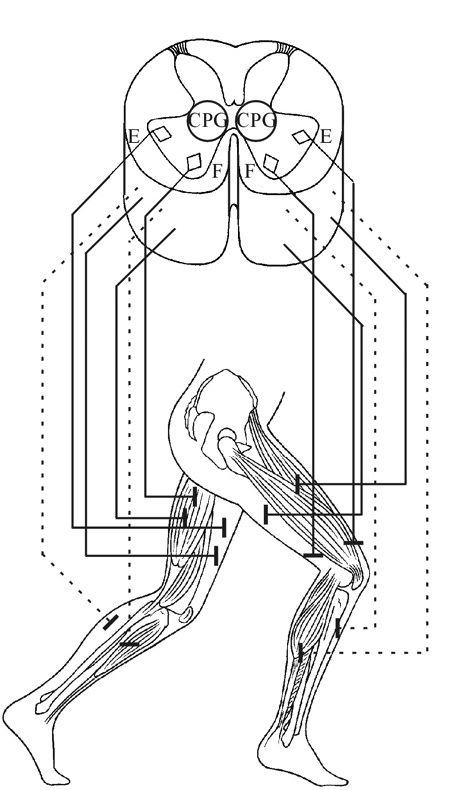
\includegraphics[width=5cm]{graphics/cpg_in_walking0.png}
		\caption[Spinal Central Pattern Generators.]{\textbf{Spinal Central Pattern Generators.} \acp{CPG} in the spine that generate rhythmic activity for locomotion without sensory or descending inputs \cite{Lacquaniti1999}}
		\label{fig:cpg_in_walking}
\end{figure}
%See also: http://www.intechopen.com/books/biomechanics-in-applications/mammalian-oral-rhythms-and-motor-control

% 1. Two best known neuro-muscular diseases.
\ac{PDis}\footnote{Parkinson's Disease is usually abbreviated as PD. In research involving the stomatogastric ganglion, however, the abbreviation PD is used for the pyloric constrictor neuron. For the sake of clarity, in the convention adopted for this document, PD is used for the pyloric constrictor neuron and PDis for Parkinson's Disease} and \ac{HD} are probably two of the best known neuromuscular diseases, and are characterised by extremely debilitating impairment of movement. The one thing that these conditions have in common is the destruction of the nerves from the brain that control the \acp{CPG} involved in movement. It is known that \ac{PDis} is caused by the death of dopaminergic neurons; that is, neurons that produce \ac{DA}, which are located in the substantia nigra, a region in the mid-brain \cite{Jankovic2008}. Motor control projections starting from the brain can also be damaged by spinal cord injury or surgery as treatment for conditions such as cancer. % 2. Spinal cord damage

% 3. CPGS are at the core of neuro-muscular control
Walking, running and swallowing are tasks that can be performed without thinking about it. These tasks are made possible by specialised neural networks that are organised in such a way that they can continually repeat particular actions. Known as \acp{CPG}, the circuits produce motor patterns controlling the muscles that allow organisms to produce repetitive movements \cite{Duysens1998, Frigon2011, Marder2005}. The rhythmic patterns produced by \acp{CPG} cannot be explained solely by anatomical connections, but are rather a product of the intrinsic properties \cite{Calabrese1998} of neurons and synaptic interactions. A diversity of patterns is essential for an appropriate response of the network to the changing environments in which organisms find themselves \cite{Selverston1998, Abbott1991}. For optimal performance in changing environmental conditions the patterns need to be adjustable, and this flexibility is provided by sensory and modulatory inputs to the \ac{CPG}.

Although \acp{CPG} can produce rhythms without external input, external inputs allow changes in rhythm for control of, or adaptation to, a changing environment. For instance, it has been found in studies using rats with spinal cord injuries that efficiency in voiding of the bladder is significantly reduced due to disruption of the phasic activity of the external urethral sphincter \cite{Dolber2007}. Treatment with 8-OH-DPAT \footnote{8-OH-DPAT is a chemical that is used to study the function of the 5-HT$_{1A}$ receptor. 5-HT$_{1A}$ is a sub-type of the serotonin (5-HT, 5-hydroxytryptamine) receptor.} \note{Wikipedia: 8-OH-DPAT is a research chemical of the aminotetralin chemical class which was developed in the 1980s and has been widely used to study the function of the 5-HT1A receptor. It was one of the first major 5-HT1A receptor full agonists to be discovered.} showed an increase in micturition volume and a decrease in residual volume resulting from improved voiding efficiency. The improved voiding efficiency can be explained by the induced emergence of phasic external urethral sphincter relaxation. The higher control of the \ac{CPG} that in turn controls the external urethral sphincter is thus severed in spinal cord injury allowing the \ac{CPG} to rhythmically open and close the sphincter much more frequently. The frequent relaxation of the sphincter, in turn, is the cause of the decreased efficiency of voiding of the bladder \cite{Dolber2007}. 


\section{Neuromodulators}
% 4a. The role of neuromodulators
Many diseases are associated with the dysfunction of systems producing neurotransmitters. For example, conditions such as schizophrenia, \ac{PDis} and \ac{ADHD} can, at least in part, be attributed to the body malfunctioning in the production of \ac{DA}. Many systems are affected in very different ways by neuromodulators. Exactly how systems are effected is not always known. Because of the complexity of such systems, research into these diseases is greatly facilitated by the use of model organisms and computational models.

\section{Models}
% 4b. Models are needed
Since it is not always possible to study the causes of diseases or the effect of injuries \textit{in vivo}, we resort to alternatives such as animal model systems, and computational models to find possible causes for a range of conditions and solutions to the problems they produce.

%\note{http://sciencelearn.org.nz/Contexts/The-Noisy-Reef/Science-Ideas-and-Concepts/Scientific-modelling}
A model, in science, is a human construct to help us understand real world systems. Models are used to explain phenomena that cannot be experienced directly. Models can be used to explain complex data, or for generating a hypothesis. Models can also be used for prediction. It is thus very important to select an appropriate type of model for the research at hand.

Animal models are usually selected for their relative tractability compared to that of humans. For instance yeast, \textit{Saccharomyces cerevisiae}, and zebra-fish, \textit{Danio rerio}, are useful for interpreting and understanding the functional and structural mechanisms of human DNA sequences. The genes, the ribosomes and cytoskeletons of \textit{S. cerevisiae} was found to be homologous to that of mammals \cite{Botstein1997, Dooley2000}. Two well-known invertebrates are the fruit fly, \textit{Drosophila melanogaster}, and the nematode worm, \textit{Caenorhabditis elegans}, which serve as model organisms in genetics, genomics and neuroscience. \textit{C. elegans}, for instance, has been favoured as a model organism since the early 1970s due to its experimental amenability, its small well-defined nervous system, the ease with which it can be genetically manipulated and the low cost maintenance \cite{Sengupta2009}.

Computational models are mathematical models of systems such as are found in biology, physics, weather systems etc. Such models can be used to predict the behaviour of these systems in an effort to develop interventions which help to control our environment. By predicting weather systems we can safeguard ourselves against extreme weather conditions or plan our crops to avoid failures. In physics, models serve the purpose of discovering the origins of the universe and predicting what the future might hold for us\note{vague}. In biology, computational models serve to provide a better understanding of the way our bodies work as part of our effort to fight disease and prolong life\note{references}.

The difficulty of building a computational model does not only lie in the creation of the model but also in the selection of parameters and the limitations placed on these parameters to keep the model biologically plausible.

% 5. Models at different scale
Models are built at various scales. There are models that are less detailed with regards to individual neurons but simulate whole areas of the brain. The Blue Brain Project\footnote{\url{http://bluebrain.epfl.ch/}}, for instance, aims to reconstruct the human brain, piece by piece, using a supercomputer to build a virtual brain. The project has already succeeded in simulating a rat cortical column. Such a cortical column has in the range of 10000 neurons and there are about 10000 columns in the cortex of the rat brain. A model such as this, however, simulates each of the neurons in less detail, due to the extensive computing resources required.

There are very detailed models of individual neurons, such as the model created by Hodgkin and Huxley that gives a detailed explanation of how \note{ explain what action potentials are} action potentials are generated and propagated \cite{Hodgkin1952a}. An action potential, sometimes referred to as a spike, is a transient reversal in polarity of the transmembrane potential in a neuron \cite{Barnett2007}. The original Hodgkin-Huxley model is a single compartment model with provision for the three main ion channels responsible for the currents that result in action potentials. This model, however, is easily extendible into multiple compartments and as many ion channels, gap junctions and synapses as are required by the system being modelled. Some of the main problems with detailed models \note{such as Hodgkin-Huxley models???} are computing requirements, the task of finding appropriate solvers for the differential equations used and, perhaps the biggest issue, finding the right parameters for the model.% say something why HH-style conductance based models are good in particular (e.g. they capture more realistic detail than larger scale models)

%6 modelling the STG
The large ganglion in the \ac{STNS} of decapod crustaceans, the \ac{STG} has proved to be an ideal system for studying the effect and impact of neurotransmitters on the generation and variation of rhythmic motor patterns produced by \acp{CPG}. This ganglion consists of about thirty neurons and form two \acp{CPG}, namely the pyloric and the gastric mill \acp{CPG}. These \acp{CPG} control muscles involved in chewing and filtering of food by producing rhythmic patterns. The \ac{STG} is well studied, and the complete connectome of all the neurons in the ganglion is known. The \ac{STG} system is not only ideal for biological research but also for the verification of computational models \cite{Harris-Warrick1992, Selverston2008}. 

Several detailed computer models of \ac{STG} sub-circuits involving a few neurons have been created \cite{Soto-Trevino2005, Golowasch1999a} - we note that these models often simulate multiple neurons of the same kind by a single model neuron (e.g. \ac{PY} or \ac{PD} neurons). Some of the models have been able to show what the effect of neuromodulators on individual neurons and the pyloric rhythm is. These models are still scaled down and model the two \acp{PD} and four to eight \acp{PY} as one \ac{PD} and one \ac{PY}. It is thus not possible to see, from the existing models, what the effect of \ac{DA} would be on the individual \ac{PD}s and \ac{PY}s.

\begin{figure}[H]
	\centering
		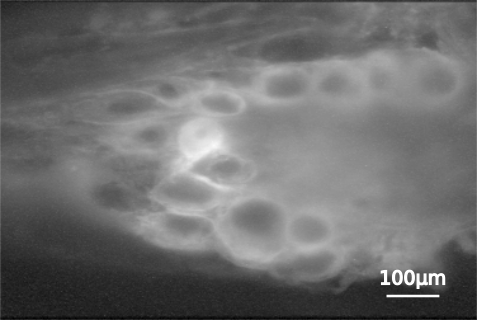
\includegraphics[]{graphics/stg_vsd.png}
		\caption[The crab stomatogastric ganglion.]{\textbf{The crab stomatogastric ganglion.} The circular objects are the somas of the neurons. The neurons are arranged around the neuropil which is a collection of axons projecting from the somas.} 
		\label{fig:STG1}
\end{figure}

The objectives of this research were:

\begin{itemize}
	\item To investigate the role of neuromodulation in the regulation of \ac{CPG} activity, using \ac{DA}.
	\item To create a detailed computational model of the pyloric \ac{CPG} capable of showing de-synchronisation of the \ac{PY} complex, that includes the two individual \ac{PD}s, five \ac{PY}s, the lateral pyloric neuron and the \ac{AB}, which in conjunction with the \ac{PD}s serves as a pacemaker group for the pyloric \ac{CPG}.
	\item To accurately model the effect of \ac{DA} on the \acp{PY} in the \ac{STG} of \species{Cancer pagurus}.
	\item To develop numerical methods to quantify measured changes when using electrophysiology and \acp{VSD} such that the output of the biological system can be compared with the output of the computational model.
	\item To investigate alternative methods of simultaneously recording from multiple neurons with the aim of getting better insight into the changes and contributions of individual neurons to the pyloric rhythm under neuromodulatory conditions. These alternative methods are considered for use in conjunction with, or in the place of existing electrophysiological and \ac{VSD} methods currently used on the \ac{STG} to improve quantification of neural behaviour for implementation in computational models.
\end{itemize}

\section{Research Approach}
Using existing models based on the Hodgkin-Huxley equations, a model was developed to include five \ac{PY} neurons, two \ac{PD} neurons, an \ac{AB} neuron and a \ac{LP} neuron. Each neuron was modelled with two compartments. One compartment represents the soma, primary neurite and dendrites and a second compartment represents the axon. All axons were modelled with three currents, $I_{Kd}$, a delayed rectifier current, $I_{Na}$, a fast sodium current and $I_{L}$ a leak current. Parameters for the model were selected from the literature.

In conjunction with the development of the model, electrophysiological recordings and voltage sensitive dye imaging were done on the dissected \ac{STNS} of brown crabs (\textit{Cancer pagurus}). The experiments were designed to provide recordings of the system before, during and after neuromodulation with \ac{DA}.

All methods of recording have some shortcomings. For instance, when using micro-electrodes the number of simultaneously recorded neurons is limited by the physical size of the micro-manipulators. It could also take quite a while to locate the appropriate neurons that is required for an experiment. Neurons are not always located in the same place and therefore, the neurons have to be impaled and recorded from, one by one, until the right one is found. During this process there is always a risk of damaging neuronal cell membranes \cite{Staedele2012}. The use of intra-cellular recording using \ac{VSD} carries the same risk and can be overcome by the use of bath-applied \ac{VSD}. The main drawbacks of all \acp{VSD} are low responsivity, signal to noise ration and toxicity. 

We thus investigated alternative methods that can be used on their own or in conjunction with existing methods, for recording neural activity. The methods investigated are:

\begin{itemize}
	\item Newly developed voltage sensitive dyes
	\item The use of multi-electrode arrays on the \ac{STG}
	\item Injection of dyes using compressed air.
\end{itemize}

The structure of this thesis is as follows. Chapter \ref{chap:background} provides background knowledge of central pattern generators, neuromodulation, existing models and modelling techniques. Chapter \ref{chap:methodsAndMaterials} provides a brief description of the general methods and materials used in the crab laboratory. Chapter \ref{chap:analysis} introduces the methods we developed for the analysis of \ac{VSD} recordings. Following this, we discuss the computational model in chapter \ref{chap:modelling}. 

Two newly developed \acp{VSD}, existing \acp{MEA} recording devices and compressed air injection are methods that have not previously been used on the \ac{STG}. In chapter \ref{chap:alternative} the possibility of successfully using these alternative methods for recording from multiple neurons in the \ac{STG} at the same time are discussed. 


Finally our conclusions and perspectives are presented in chapter \ref{chap:conclusions_perspectives}. 

The \matlab source code of the model can be downloaded from \url{http://www.jannetta.com/downloads/PYCPG_model.zip}



%Introduction
	\chapter{Background}
\label{chap:background}
	
\section{Central Pattern Generators}

Underlying the production of most rhythmic motor patterns are \acp{CPG} \cite{MacKay-Lyons2002}. The earliest hints at the existence of \acp{CPG} came from experiments performed on cats by Sherrington and Brown \cite{Sherrington1910, Brown1911}. Brown noticed: ``a mechanism confined to the lumbar part of the spinal cord is sufficient to determine in the hind limbs an act of progression'' \cite{Brown1911a}. The first modern evidence of centrally generated motor pattern was demonstrated in the locust nervous system by Wilson. He showed that, when isolated from the animal, the nervous system could produce rhythmic output that resembles the neural activity observed during flight \cite{Wilson1961, Hooper2001, Marder1996}. Now known as \acp{CPG} the existence of groups of neurons that produce rhythmic patterns, independently of peripheral afferent feedback, is indisputable \cite{MacKay-Lyons2002}. Although not yet conclusive, there is some evidence to support the presence of spinal \acp{CPG} in humans \cite{Dimitrijevic1998}. Banaie \cite{Banaie2009}, presented a model for \ac{HD} gait disorder. The model is based on the hypothesis that \ac{CPG} circuits are established in some neuromuscular diseases which then produce semi-periodic movements. In a normal person, variation in the gait signal appears to have a random-like behaviour. In \ac{HD} patients a semi periodic signal is observed which is the result of some oscillations of the \ac{CNS} being synchronised to produce the movement symptom \cite{Banaie2009}.

Basic principles of \ac{CPG} function is mostly based on research in invertebrates and primitive vertebrates such as the lamprey \cite{Grillner2005}. Later research include studies of the axial \ac{CPG} in the salamander \cite{Ryczko2015}.

The rhythmic patterns produced by \acp{CPG} are often involved in vital functions such as breathing, walking, flying and chewing \cite{Marder2001}. A simple oscillating circuit can be produced from as little as two neurons each of which inhibits the other. However, many inherent factors of a circuit, such as cellular properties, synaptic properties and network connectivity patterns, can contribute to the generation and characteristics of a pattern. Hooper identifies two things that are required to produce rhythms: \textit{``(1) two or more processes that interact such that each process sequentially increases and decreases, and (2) that, as a result of this interaction, the system repeatedly returns to its starting condition.''}. There are two mechanisms for producing neural rhythmicity; (1) either there are interactions among neurons or (2) there are interactions among electrical currents in individual neurons \cite{Hooper2001}. 

Network-based rhythmicity occurs when there are interactions among neurons with no rhythmogenic ability. When reciprocally coupled these neurons form half centre oscillators that produce rhythmic outputs. An example of such a half-centre oscillator based system is the heartbeat network of the leech \species{Hirudo medicinalis} \cite{Norris2006}.

Endogenous oscillator neurons, are neurons that could, even when isolated from a network, continue to depolarise to the point where they fire action potentials, re-polarise and then repeat the cycle again. The rhythm produced by such oscillator neurons is the result of membrane currents. An example of such a neuron is the \ac{AB} in the pyloric network located in the \ac{STG} of crustaceans. This \ac{CPG}, as the subject of this research, will be discussed in more detail later.

Circuits driven by both mechanisms, network based rhythmicity and endogenous oscillator driven networks, can be multifunctional. Multi-functionality is provided by modulatory mechanisms that can alter the properties of the neurons involved in rhythmic circuits \cite{Getting1989}. The term "polymorphic network" was coined by Getting and Dekin \cite{Getting1985} to define a network that could be organised into multiple states or configurations. Each of these states or configurations are called "circuits" and each circuit produces a different motor pattern \cite{Getting1985a}. 

To understand the workings of \acp{CPG} it is useful to use model biological systems that are significantly simpler than those of mammals \cite{Abbott1998}.  The benefit of small systems is that they can be used to generate hypotheses about how processes might occur in more complex systems. Furthermore, the existence of \acp{CPG} in humans still lacks final proof and thus relies on research using reduced models \cite{Iosa2015}.

Before looking into the \ac{STG} in more detail it is worth considering some other model systems. To this end a short discussion of \species{Tritonia}, \species{Lymnaea} and \species{Hirudo medicinalis} follows to illustrate some of the basic concepts of \acp{CPG}

\section{\Ac{CPG} model species}
\subsection{The leech, \species{Hirudo medicinalis}, heartbeat network}
 
The leech has two hearts that are driven by heart (HE) motor neurons. The heart motor neurons are paced by a \ac{CPG} network of seven identified bilateral pairs of segmental \acp{HN} and one, as yet, unidentified pair of heart inter-neurons (HN(X)), that produce rhythmic activity at a rate of about 0.1 Hz. Synaptic activity between inter-neurons and from the inter-neurons to the motor neurons are inhibitory \cite{Hill2002, Norris2007}. The heartbeat is coordinated by reciprocal inhibition between the \ac{HN} cells. See figure \ref{fig:leech}

\begin{figure}[H]
	\centering
		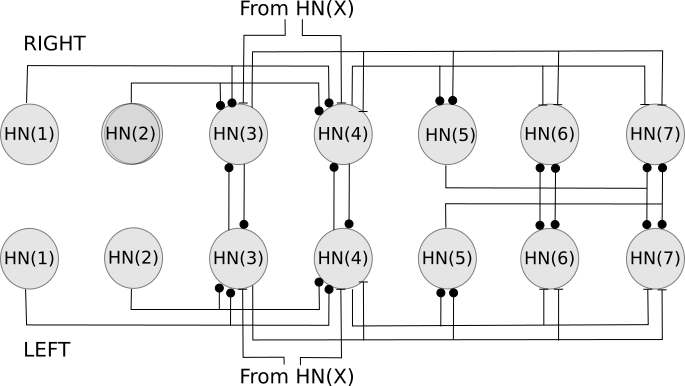
\includegraphics[width=\columnwidth]{graphics/leech.png}
		\caption[The Leech Heartbeat.]{\textbf{The Leech Heartbeat.} A network diagram of the leech heartbeat \ac{CPG} showing known synaptic connections between heart inter-neurons. HN(1) to HN(7) are the identified inter-neuron pairs while HN(X) is the unidentified neuron pair. All synapses are inhibitory except for the connections from HN(X) to HN(3) and HN(4). Adapted from \cite{Calabrese1977}.}
		\label{fig:leech}
\end{figure}


\subsection{\species{Tritonia}}
\species{Tritonia} is a gastropod mollusc. The swim \ac{CPG} of \species{Tritonia} has been a model system for studying rhythmic motor pattern generation for many years. The \species{Tritonia} swim \ac{CPG} is also a  network oscillator in that it has no neurons with intrinsic burst properties. Rhythmic bursting arise through conventional synaptic interactions. This \ac{CPG} is initiated by sensory input which results from contact with the tube feet of certain predatory sea stars \cite{Getting1985}.

The swim \ac{CPG} consists of the \ac{C2}, the \ac{DSI} and two types of \acp{VSI}. In a basic scenario the swim motor pattern is initiated by sensory input that activates \ac{DRI}. \ac{DRI} excites \ac{DSI} which, in turn, excites \ac{C2}. \ac{C2} feeds back and excites \ac{DRI}, which then further excites \ac{DSI} via a positive feedback loop. \ac{C2} excites \acp{VSI}, which then inhibits \ac{DSI} and \ac{C2}, thus momentarily interrupting the positive feedback loop. Figure \ref{fig:Tritonia_swim_CPGcircuit} shows the \species{Tritonia} swim \ac{CPG} circuit. The figure also shows the S-cells which are both mechanoreceptive and chemoreceptive. Excitaton of the S-cells are conveyed onto the Tr1 and \ac{DRI} cells via excitatory glutamatergic synapses \cite{Frost1996, Katz2009}).

\begin{figure}[H]
	\centering
	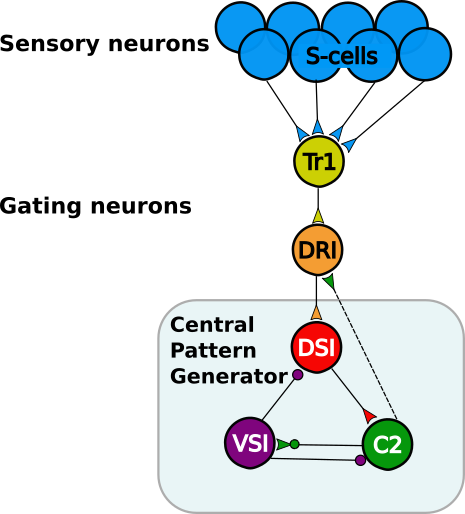
\includegraphics[width=9cm]{graphics/Tritonia_swim_CPGcircuit.png}
	\caption[The \species{Tritonia} swim \ac{CPG}.]{\textbf{The \species{Tritonia} swim \ac{CPG}}. This circuit shows the synapses involved in the  Circles represent inhibitory synapses and triangles represent excitatory synapses. Combinations of circles and triangles represent multicomponent synapses. (Adapted from \cite{Katz2009})}
	\label{fig:Tritonia_swim_CPGcircuit}
\end{figure}

The \acp{DSI} not only activate \ac{C2} synaptically but also via neuromodulation. Both the synaptic and neuromodulatory activation are mediated by serotonin (5-HT), which is released by the \ac{DSI} \cite{Katz1995, Katz1997}.

Some of the neurons in the swim \ac{CPG} of \species{Tritonia} have been found to be multi-functional in that they have functions other than just being involved in swimming. The \acp{DSI}, for example, excite neurons in the pedal ganglia that increase the speed of crawling \cite{Popescu2002}. Getting and Dekin used \species{Tritonia} as an example of a "polymorphic network" \cite{Getting1985a}.

\subsection{\species{Lymnaea}}
Yet another model organism which provides us with two more interesting \ac{CPG} networks for study is \species{Lymnaea stagnalis}, the pond snail. These \acp{CPG} are found in the feeding (see figure \ref{fig:Lymnaea_feeding_network}) and respiratory networks (see figure \ref{fig:Lymnaea_respiratory_network})  \cite{Kemenes2009}.

The name of \species{Lymnaea stagnalis} is deduced from the fact that it lives in stagnant water. The stagnant water leads to a hypoxic environment at which causes the snails to surface and perform rhythmic opening and closing movement of the pneumostome (the pulmonary opening). These movements are controlled by the respiratory \ac{CPG} \cite{Benjamin2008}. The \ac{RPeD1} initiates the respiratory rhythm while the \ac{IP3} causes the pneumostome to open (i.e. expiration) and the \ac{VD4} causes it to close (i.e. completion of inspiration). \ac{IP3} is connected to the I/J motoneuron via a monosynaptic excitatory connection. The activity of I/J causes the pneumostome to open. \ac{VD4} is connected to the K motoneuron, also via a monosynaptice excitatory connection. The activity of K causes the the pneumostome to close  \cite{Taylor2000}.

As in the case of \species{Tritionia} it has been found that many \species{Lymnaea} neurons are multifunctional \cite{Syed1991a, Kemenes2009}. For example, \ac{RPeD1}, a respiratory \ac{CPG} neuron has been found to co-ordinate sensory-motor input from the pneumostome at the water/air interface to initiate respiratory rhythm generation \cite{Haque2006}.

 \begin{figure}[H]
 	\centering
 	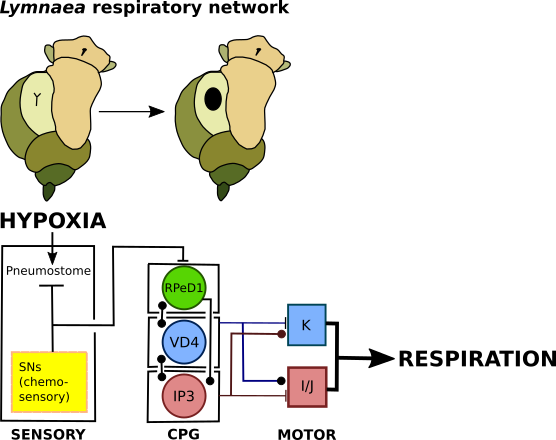
\includegraphics[width=\columnwidth]{graphics/lymnaea_b.png}
 	\caption[\species{Lymnaea respiratory network}]{\textbf{The \species{Lymnaea} respiratory \acp{CPG}}. The filled circles are inhibitory chemical synapses while the vertical bars indicate excitatory chemical synapses. Hypoxic conditions in stagnant water evokes compensatory changes in respiration. The \ac{CPG} consists of three neurons: 1) the \ac{RPeD1} which initiates the respiratory rhythm, 2) the \ac{IP3} which causes the pneumostome, via an excitatory monosynaptic connection to I/J, to open and 3) the \ac{VD4} which causes the pneumostome to close via the excitatory monosynaptic connection to K. (Adapted from \cite{Benjamin2008})}
 	\label{fig:Lymnaea_respiratory_network}
 \end{figure}
 
\species{Lymnaea} possesses a toothed radula which is used for feeding. Feeding consist of the mouth begin opened and the radula being scraped over the food substrate. The food is lifted into the mouth and the mouth is then closed while the food is swallowed. These movements are repeated while the snail is feeding. The rhythmic movements of the feeding muscles are driven by motorneurons which in turn are driven by synaptic inputs from the feeding \ac{CPG}.

The \ac{CPG} interneurons are divided into three main classes, N1, N2, and N3. The classification is made according to the phase of the feeding pattern, i.e. protraction, rasp (or retraction) and swallow. These neurons provide  sequences of excitatory and inhibitory synaptic inputs to motorneurons involved in the three phasic feeding rhythm. The rhythmic activity of the \ac{CPG} relies on both synaptic connections and intrinsic electrical properties of the N neurons \cite{Vavoulis2007}. Activity in the \ac{CPG} neurons and in the motoneurons are modulated by higher order interneurons such as the \ac{CGC}, \ac{SO} and \ac{CBI}. 

The frequency of the feeding \ac{CPG} is controlled by the \ac{SO} via know synaptic connectivity. The \ac{SO} is extrinisic to the \ac{CPG}. The rhythm is driven by a steady depolorisation of the N1 cells. Brief stimulation of N2 and N3 resets the phase of the rhythm. The N1 neurons excite the N2 interneurons which in turn inhibit the N1 cells \cite{Elliott1985}.

 \begin{figure}[H]
 	\centering
 	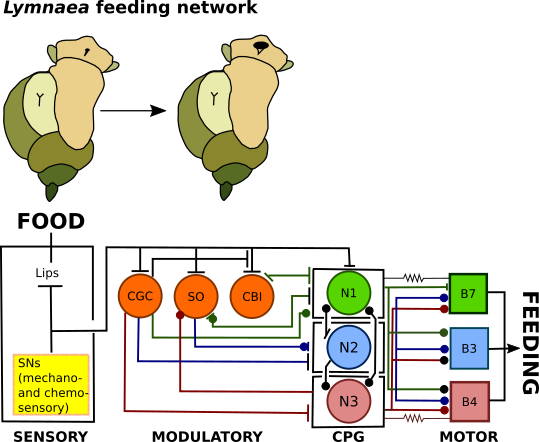
\includegraphics[width=\columnwidth]{graphics/lymnaea_a.png}
 	\caption[\species{Lymnaea feeding network}]{\textbf{The \species{Lymnaea} feeding \acp{CPG}}. The filled circles are inhibitory chemical synapses while the vertical bars indicate excitatory chemical synapses. Resistor symbols indicate electrical synapses. B7, B3 and B4 are motoneurons. Neurons N1, N2 and N3 form the \ac{CPG}. B7, B3 and B4 are motoneurons. The activity of all these neurons are modulated by higher order neurons such as the \ac{CGC}, \ac{SO} and \ac{CBI}. (Adapted from \cite{Benjamin2008})}
 	\label{fig:Lymnaea_feeding_network}
 \end{figure}

\section{The Crustacean Stomatogastric Nervous System}
The model system chosen for this research was the previously mentioned pyloric network found in the \ac{STG} which is located in the \ac{STNS} of crustaceans. In the case of the \ac{STG}, forming hypothesis of processes in more complex systems can be done by demonstrating in detail how cellular infrastructure produces rhythmicity and specialised patterns \cite{Selverston2010}.

The \ac{STNS} has been a tool for research into neural circuit dynamics for more than 40 years and a number of different crustacean species have been employed. These species include spiny lobsters (\species{Panulirus argus} and \species{Panulirus interruptus}), clawed lobsters (\species{Homarus americanus} and \species{Homarus gammarus}), various crab species (\species{Cancer borealis} and \species{Cancer pagurus}), crayfish and shrimp \cite{Marder2007}.

A detailed description of the gross anatomy of the stomatogastric system is beyond the scope of this thesis. There is, however, an extensive literature available on this subject, of which the writings of Selverston, Maynard and Dando \cite{Selverston1976,Maynard1973} are probably the most prominent.

In crustaceans the \ac{STNS} (Fig: \ref{fig:location_STNS} and \ref{fig:STNS}) is an extension of the central nervous system, controlling the foregut by innervating the striated muscles that produce rhythmic movement in the oesophagus, cardiac sac, gastric teeth and the pyloric chamber \cite{Selverston1987}. It consists of four ganglia: the \ac{OG}; the paired \acp{CoG}; and the \ac{STG}. The \ac{OG} contains about 18 neurons, while each of the \acp{CoG} contains about 400 neurons \cite{Marder2007}.

\begin{figure}[H]
	\centering
		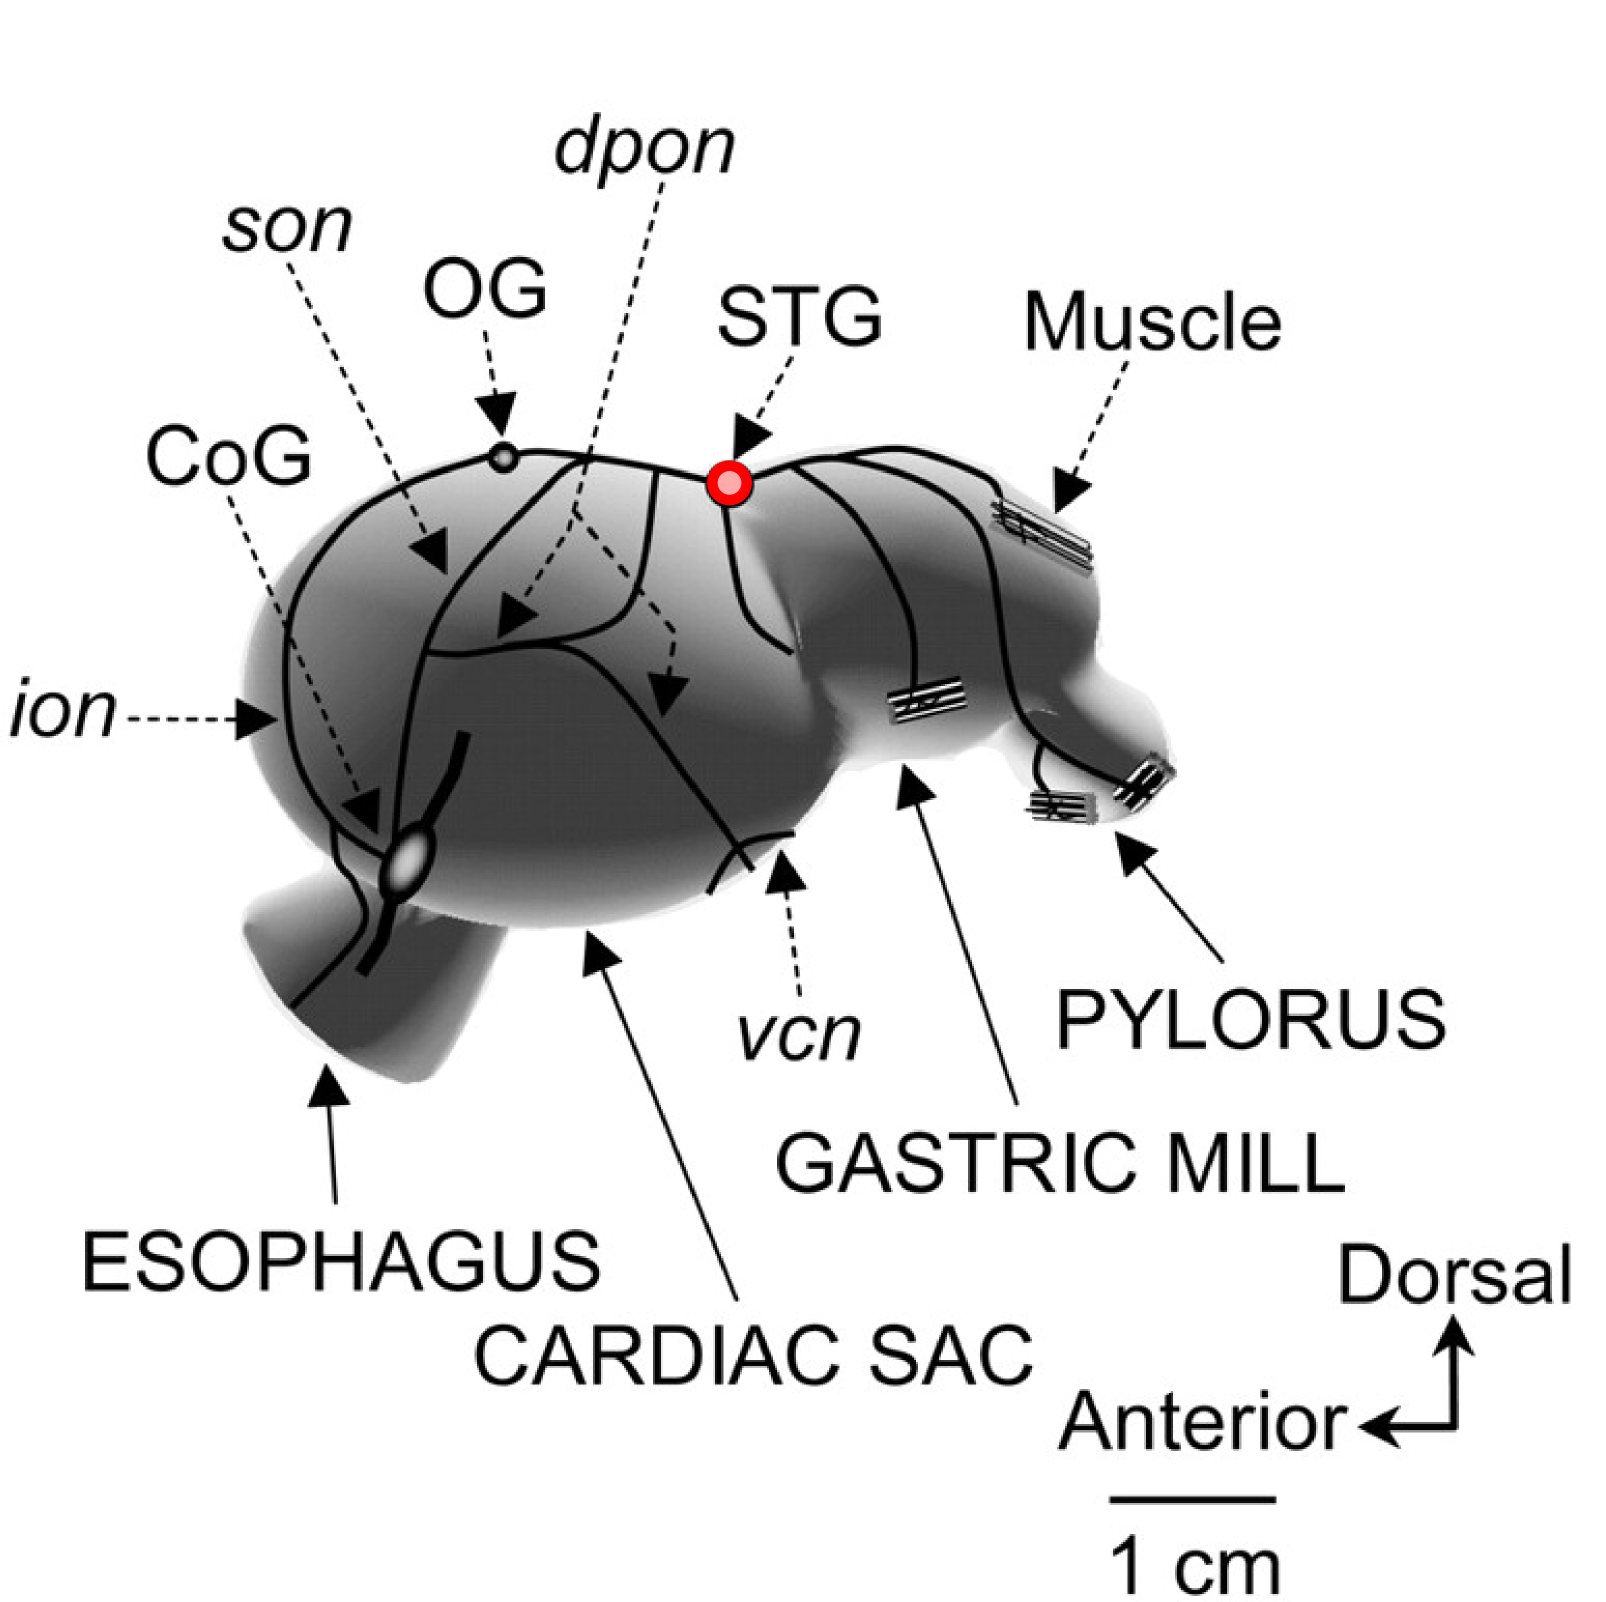
\includegraphics[width=9cm]{graphics/foregut_stns_beenhakker.png}
		\caption[Location of the crab \ac{STNS} around the stomach.]{\textbf{Location of the crab \ac{STNS} around the stomach.} Shown is the innervating \ac{STNS}, in black, and the \ac{STG}, in red, around the crab foregut. Arrows with dotted lines point to \ac{STNS} elements which include the \ac{ion}, \ac{CoG}, \ac{son}, \ac{OG}, \ac{dpon}, \ac{STG}, a muscle and the \ac{vcn}. Arrows with solid lines point to foregut regions (Adapted from \cite{Beenhakker2004})} 
		\label{fig:location_STNS}
\end{figure}

The underlying circuitry of the \ac{STNS} is well known. Figure \ref{fig:stns_connectome} shows the pyloric and gastric circuits that comprise the lobster stomatogastric nervous system.

\begin{figure}[H]
	\centering
		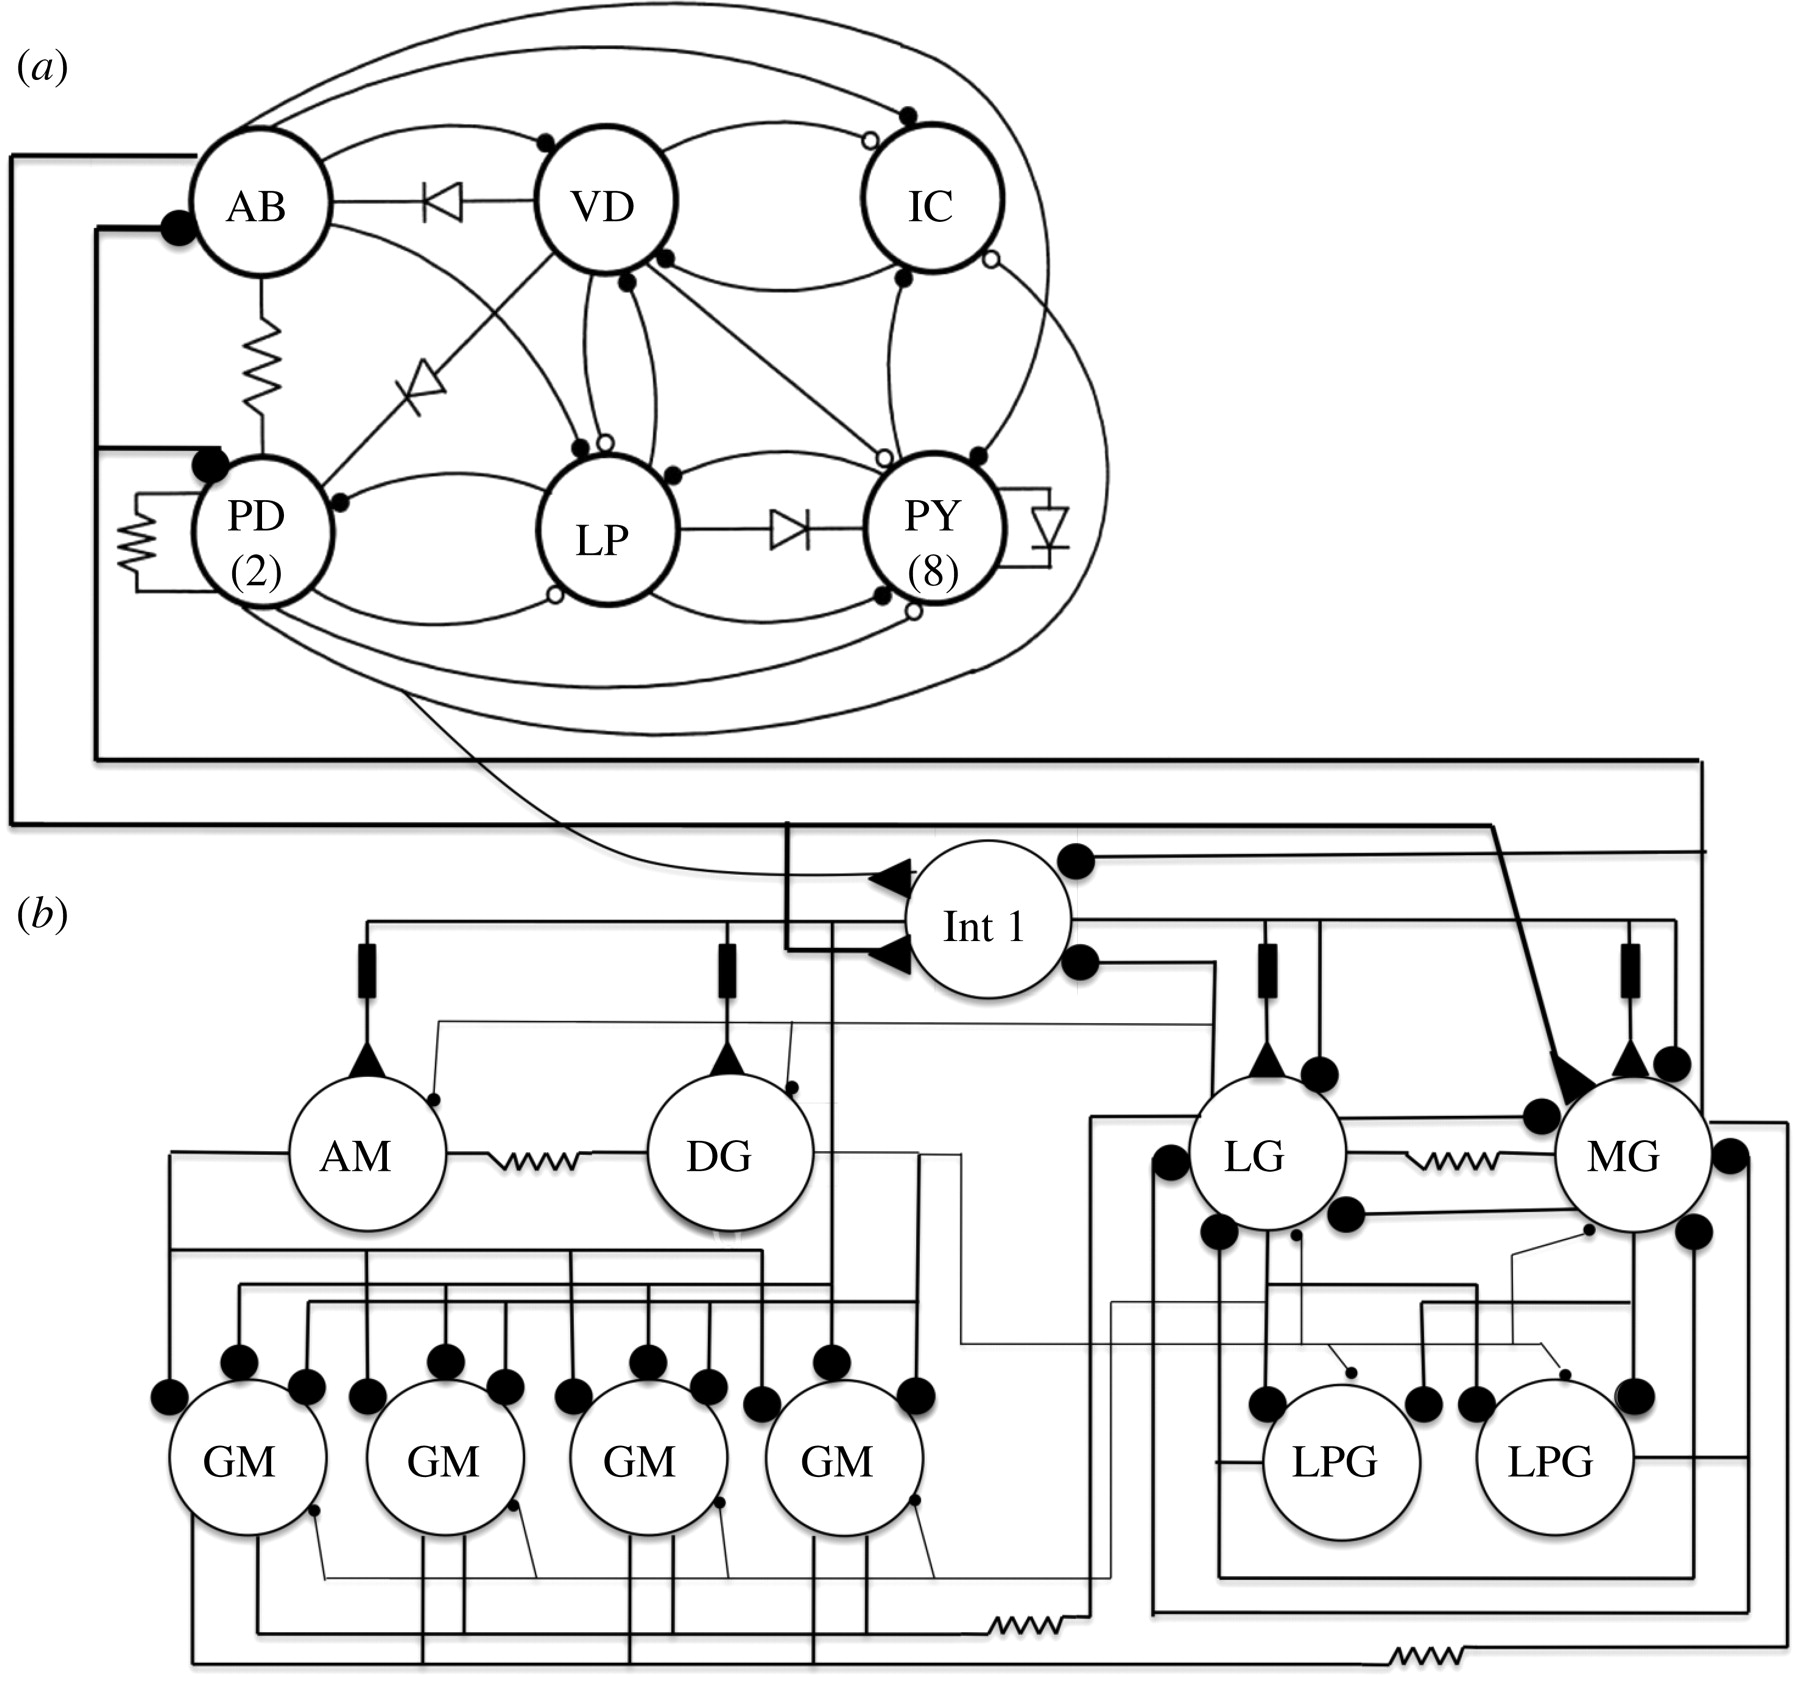
\includegraphics[width=\columnwidth]{graphics/stns_connectome.png}
		\caption[The underlying circuitry of the lobster stomatogastric network.]{\textbf{The underlying circuitry of the lobster stomatogastric network.} Symbols: large circles, neurons; black dots, inhibitory synapses; triangles, excitatory synapses; resistors, electrical coupling and diode symbols,  rectifying electrotonic connections. The rectangles represent delay lines between spikes in the presynaptic neurons and postsynaptic excitatory repsonse. Adapted from \cite{Selverston2010}}
		\label{fig:stns_connectome}
\end{figure}

\begin{figure}[H]
	\centering
		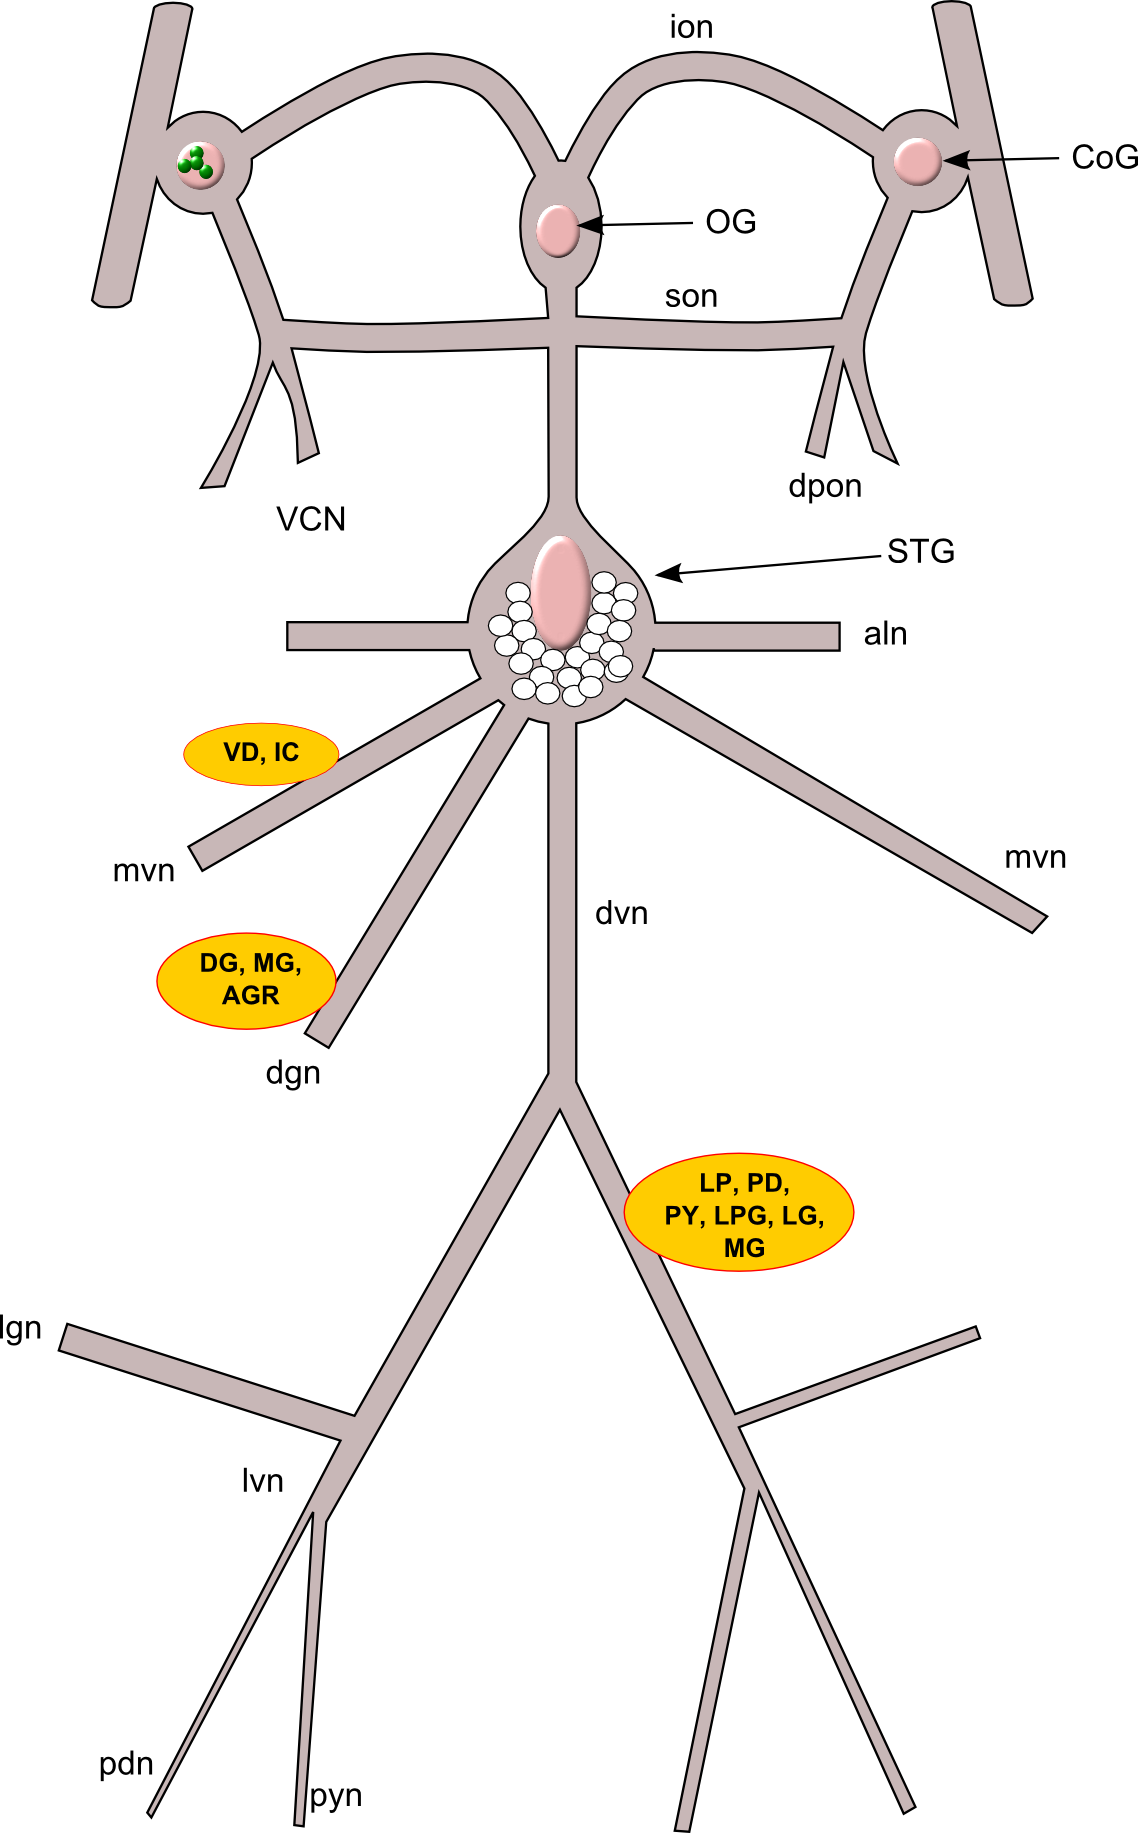
\includegraphics[width=9cm]{graphics/STNS.png}
		\caption[The stomatogastric ganglion.]{\textbf{The Stomatogastric Ganlgion.} A diagram of the stomatogastric nervous system (STNS) showing the commisural ganglia (CoG), the oesophageal ganglion (OG), the \ac{STG} (STG) and all interconnecting nerves (ion, son, dpon, stn, vcn, aln, mvn, dgn, dvn, lgn, lvn, pdn, pyn). Lower case abbreviations are used for the nerves while capitalised abbreviations are used for neurons. All neurons (AB, AM, AGR, DG, GM, Int1, LG, LP, LPG, PD, MG, PY, VD) are located in the stomatogastric ganglion (STG). The axons of neurons projecting down specific nerves are shown in the orange circles. }
		\label{fig:STNS}
\end{figure}

\section{The Stomatogastric Ganglion}

The \ac{STG} is found on the dorsal surface of the foregut of decapod crustaceans (Fig: \ref{fig:location_STNS}). The ganglion consists of 24-26 neurons in crabs and 29-32 neurons in lobsters. These neurons form two \acp{CPG}, the pyloric and gastric mill \acp{CPG}. Differences in the number of \acp{GM} and \acp{PY} between species account for the variability in the number of neurons \cite{Marder2007}.

\begin{figure}[H]
	\centering
		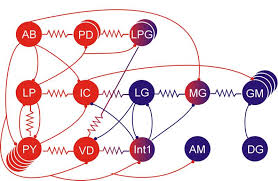
\includegraphics[width=\columnwidth]{graphics/stg.jpg}
		\caption[Neurons of the stomatogastric ganglion.]{\textbf{Neurons of the stomatogastric ganglion} with all inhibitory and electrical synapses indicated. Inhibitory synapses are shown as circles on the neuron that is inhibited. Electrical synapses are indicated by the resistor symbol (a zig-zag). The circuit consists of one \acf{AB}, two \acfp{PD}, two \acfp{LPG}, one \acf{LP}, one \acf{IC}, one \acf{MG}, four \acfp{GM}, five \acfp{PY} (which could vary between four and eight depending on the species), one \acf{VD}, one \acf{Int1}, one \acf{AM} and one \acf{DG}. (from \url{http://www.bio.brandeis.edu/marderlab//figures/circuit.jpg})}
		\label{fig:STG}
\end{figure}


The pyloric \ac{CPG} produces a cyclic three-phase rhythm that controls the striated muscles which constrict and dilate the pyloric region of the stomach. The pyloric region is a section of the foregut that is responsible for the filtering of masticated food. Chewing is controlled by a six-phase rhythm produced by the gastric mill \ac{CPG} \cite{Marder2001, Selverston2005, Selverston2010}, controlling the movements of two lateral teeth and one medial tooth \cite{Heinzel1993}.

However, these two rhythms are not the only output that can be generated by the \ac{STG}. The networks in the \ac{STG} are very plastic and can be reconfigured by neuromodulation to produce multiple variants of the basic rhythms. The neurons of the two \acp{CPG} can even be recruited into other motor networks \cite{Johnson2003, Nusbaum2002}.


\subsection{Neurons of the STG}
The gastric \ac{CPG} is comprised of 11 neurons. Eleven to 14 of the neurons in the \ac{STG} belong to the pyloric \ac{CPG}. The number of neurons in the pyloric \ac{CPG} varies between species and between individuals within a species \cite{Daur2012a}. The lobster (\textit{Homarus americanus}), for instance, has eight PY neurons while the crab (\textit{Cancer pagurus}) has only four or five. Compared to mammalian neurons, the neurons of the \ac{STG} have relatively large somas of 50 to 100$\mu$m in diameter \cite{Marder2007}.

Both chemical and electrical synapses are found in the \ac{STG}. All of the chemical synapses are inhibitory \cite{Selverston1987}, with the exception of those involving projection neurons. The projection neurons are located in the \acp{OG}, projecting axons down the \ac{stn} to the \ac{STG}. The \ac{STG} neurons are mostly motor neurons and make excitatory neuromuscular connections \cite{Marder1987}.

Tables \ref{tab:gastric} and \ref{tab:pyloric} give the number of each neuron, its name, abbreviation and the muscle it innervates for the gastric and pyloric \acp{CPG} respectively. The abbreviations used for the neurons, nerves and muscles are based on a convention created by Maynard and Dando in which the nerves are named after the muscle they innervate \cite{Maynard1973, Marder1979a}.

\renewcommand{\tablename}{Table}
\begin{table}
	\centering
	\caption[Neurons of the Gastric \ac{CPG}]{\textbf{Neurons of the Gastric \ac{CPG}}}
	\label{tab:gastric}
	\begin{tabular}{l l l l }
		\hline
		\bf \# & \bf Neuron name & \bf Abbr. & \bf Muscle\\ \hline
		1 & Interneuron 1 & (Int 1) & interneuron \\ 
		4 & Gastric Mill & (GM) & gm 1, 2a, b \\ 
		1 & Dorsal Gastric & (DG) & gm 4a, b, c \\ 
		1 & Anterior Median & (AM) & c6, c7 \\ 
		1 & Lateral Gastric & (LG) & gm 5b, 6a \\ 
		1 & Medial Gastric & (MG) & gm 9a, 9c \\ 
		2 & Lateral Posterior Gastric & (LPG) & gm 3 \\ 
		\hline
	\end{tabular}
\end{table}

\begin{table}
	\centering
	\caption[Neurons of the Pyloric \ac{CPG}]{\textbf{Neurons of the Pyloric \ac{CPG}}}
	\label{tab:pyloric}
	\begin{tabular}{l l l l}
		\hline
		\bf \# & \bf Neuron name & \bf Abbr. & \bf Muscle\\ \hline
		1 & Anterior Burster & (AB) & inter-neuron \\ 
		2 & Pyloric Dilator & (PD) & cpv 1 and 2 \\ 
		1 & Lateral Pyloric & (LP) & p1 \\ 
		1 & Ventricular Dilator & (VD) & cv2 \\ 
		1 & Inferior Cardiac & (IC) & cv3 \\ 
		4 - 8 & Pyloric Constrictor & (PY) & p2-4, 7-9, 1-11 \\ 
		\hline
	\end{tabular}
\end{table}

Both these \acp{CPG}
produce rhythms that can be recorded intracellularly and extracellularly. In both cases the recordings obtained from \textit{in vitro} preparations are largely indistinguishable from those obtained from intact crabs  (figure \ref{fig:pyloric_rhythm_in_vivo_in_vitro}) \cite{Hedrich2011}.

\begin{figure}[H]
	\centering
		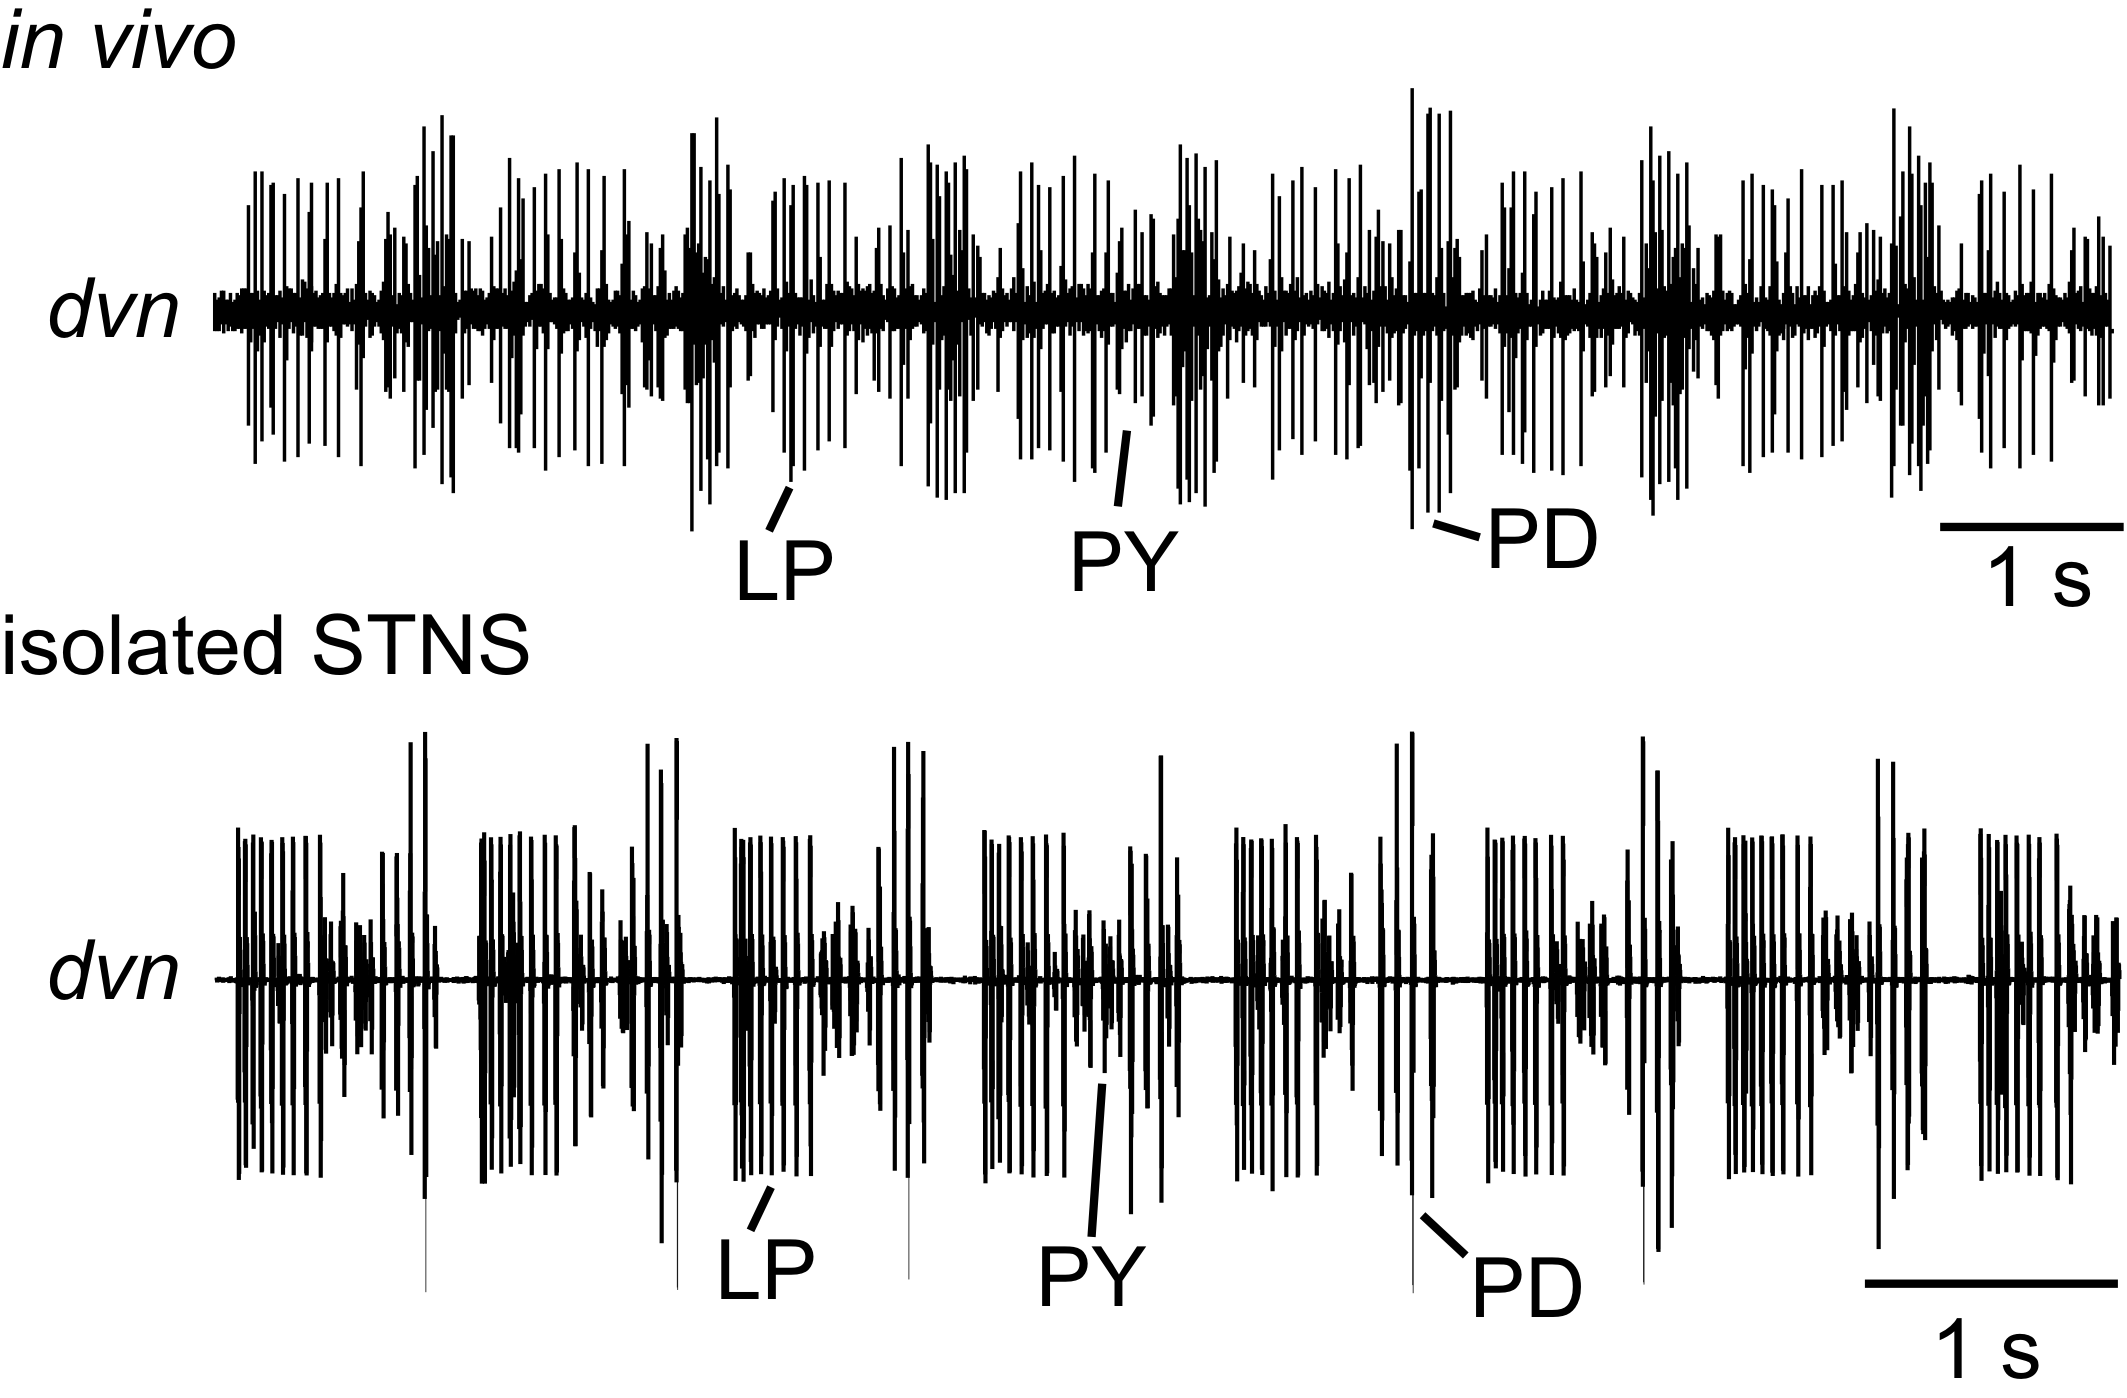
\includegraphics[width=8.5cm]{graphics/pyloric_rhythm_in_vivo_in_vitro.png}
		\caption[In vivo and in situ recordings of gastric and pyloric neurons]{\textbf{In vivo and in situ recordings of gastric and pyloric neurons} over the \ac{dvn} and \ac{mvn} in \species{Cancer borealis}. The recordings are largely indistinguishable. Adapted from \cite{Hedrich2011}, courtesy of Wolfgang Stein.} 
		\label{fig:pyloric_rhythm_in_vivo_in_vitro}
\end{figure}

%Weimann 1991
%Katz 1991

\subsection{Neurons of the Pyloric CPG}

Interneurons are neurons that form connections between other neurons while motor neurons carry signals to the muscles to produce movement. Motor neurons interface with muscles through specialised synapses known as neuromuscular junctions. Of the 11 to 14 neurons of the pyloric \ac{CPG} one is an inter-neuron, the \ac{AB}, while the rest, the \acp{PD}, \ac{LP}, \acp{PY}, \ac{VD} and \ac{IC} are motor neurons. 

% Buchholtz1992 - more about LP
%================================
There are two major classes of bursting neurons. Firstly there are constitutive bursters which rely on ionic conductances for its bursting. The second class of bursting neurons are the conditional bursters which rely on ionic mechanisms to generate rhythmic activity. 
%\when isolated these cells loose the ability to burst. Harris-Warrick1987

The \ac{AB} is an endogenous oscillator which can oscillate even when isolated from the network. The \ac{AB} is electrically connected to the \acp{PD} via gap junctions \cite{Zhao2010} to form what is known as the pacemaker group. The \ac{AB} oscillates, in conjunction with the \acp{PD}, to serve as a kernel pacemaker that drives the pyloric circuit at a rate of approximately one Hertz \cite{Soto-Trevino2005, Abbott1991}. This pacemaker group acts as the timer for pyloric rhythm. Typical of pacemaker-driven activity, the depolarisation of the \ac{AB} increases the frequency of bursting while depolarisation decreases the frequency \cite{Selverston1985}. Together the \ac{AB} and \acp{PD} inhibit the \acp{LP} and \acp{PY}. This inhibition forces the \acp{LP} and \acp{PY} to fire alternately with the \acp{PD} \cite{Bargmann2013}. The \acp{PY} take longer to rebound from inhibition than the \acp{LP}, and are therefore inhibited further by the \acp{LP}. When the \acp{PY} do rebound from inhibition they terminate the \acp{LP} \cite{Marder2007}.

The \acp{PD} drive one muscle group of the pylorus. The  \ac{LP} and \ac{PY} follower neurons drive another group of muscles. Fig. \ref{fig:pyloriccpg} shows the neurons of the pyloric \ac{CPG} and their connections with one another.

Bursting in neurons is produced by a combination of slow inward currents that produce a depolarising phase followed by activation of a slow outward current that terminates the burst. There are also faster, voltage-gated currents, which account for spikes during the depolarised phase allowing action potentials and bursting to co-exist. It has been hypothesised that Ca\textsuperscript{2+} is part of the inward current. Ca\textsuperscript{2+} accumulation activates the Ca\textsuperscript{2+}-activated K\textsuperscript{+} currents that have been shown to terminate bursts in several systems \cite{Levi2003} %check Amini et al. 1999; Kiehn and Harris Warrick, 1992



\begin{figure}[H]
	\centering
		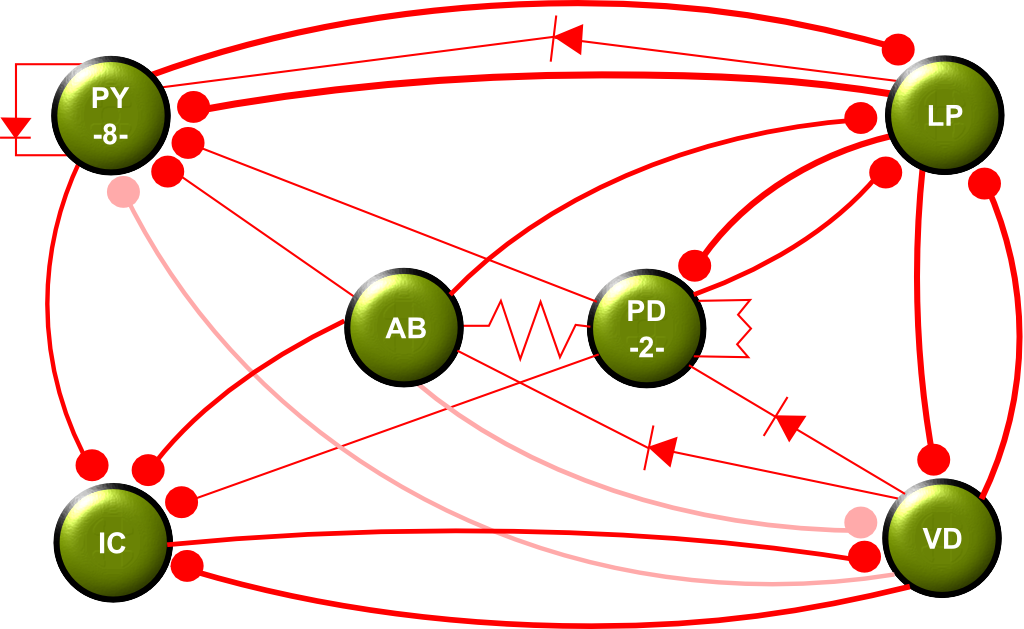
\includegraphics[width=9cm]{graphics/pyloriccpg.png}
		\caption[Neurons of the pyloric \ac{CPG}.]{\textbf{Neurons of the pyloric \ac{CPG}.} Inhibitory synapses are shown with filled circles; non-rectifying electrical synapses are shown with a resistor and rectifying synapses are shown with a diode symbol that also shows the direction of the preferred current flow. (Adapted from \cite{Harris-Warrick2011})}
		\label{fig:pyloriccpg}
\end{figure}

\subsection{Neurons of the Gastric Mill CPG}
The gastric mill \ac{CPG} also has one inter-neuron, \ac{Int1}, while the remaining neurons, the \acp{GM}, \ac{DG}, \ac{AM}, \ac{LG}, \ac{MG} and \acp{LPG} are motor neurons. The gastric mill \ac{CPG} produces a five-phased motor pattern. Chemical synapses in this \ac{CPG} are inhibitory, while electrical synapses are mostly non-rectifying. The \ac{LG} and \ac{MG} neurons fire at about the same time, and alternate with the \ac{LPG}. The \ac{DG}, \ac{AM} and \ac{Int1} fire together and alternate with the \ac{GM} \cite{Harris-Warrick1992}.

\begin{figure}[H]
	\centering
		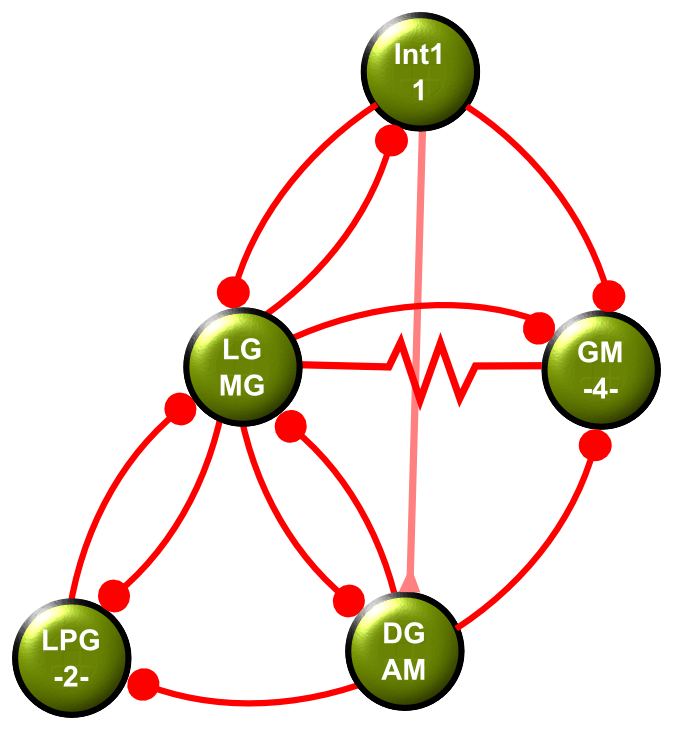
\includegraphics[width=9cm]{graphics/gastriccpg.png}
		\caption[Neurons of the gastric mill \ac{CPG}.]{\textbf{Neurons of the gastric mill \ac{CPG}}.  Inhibitory synapses are shown with filled circles; non-rectifying electrical synapses are shown with a resistor, (Adapted from \cite{Harris-Warrick1992})}
		\label{fig:gastriccpg}
\end{figure}

In crustacea, the gastric mill \ac{CPG} controls the chewing movements of three teeth located in the gastric mill \cite{Rowat1993}.

\section{Neuromodulation}
\note{ NEUROMODULATORS  CAN  ALTER  SYNAPTIC EFFICACY Harris-Warrick1991}
Despite the fact that the complete ``wiring diagram'' for the \ac{STG} has been known for more than 25 years, it was soon clear that the static connectivity diagram could not capture the dynamics of the circuit \cite{Abbott1998}. An interesting phenomenon in neural systems is their ability to maintain stability despite environmental changes. These changes include extracellular conditions as well as channel turnover and cell growth \cite{LeMasson1993}.  Flexibility to cope with such changes is provided for by sensory input, neuromodulation which tunes the intrinsic neuronal excitability and synaptic properties of neurons as well as the inputs to the circuits of which the neurons are part \cite{Bucher2013, Johnson2005, Nadim2014}. 

Neuromodulation is caused by substances known as neuromodulators, such as amines, neuropeptides, gasses and small-molecule neurotransmitters. Some neuromodulators are produced locally by the neurons while others are released remotely and transferred to neurons through the bloodstream. These molecules are known as neurohormones \cite{Stein2009}. 

The source of neuromodulators in modulated circuits can be intrinsic or extrinsic. In the latter, the cells releasing the neuromodulators are not part of the modulated circuit. Indirect feedback to the neurons of origin might, however, exist. In the former the neurons releasing the neuromodulator are part of the modulated circuit \cite{Bucher2013}.

In the \ac{STNS} all stages of the neuronal processing are affected by factors such as membrane currents, synaptic transmissions, or the properties of the effector muscles \cite{Stein2009}. At least 18 neuromodulatory substances are found in the \ac{STG} \cite{Marder1987, Marder1995, Marder2001, Marder2007}, and the same neuromodulator can differently affect pyloric neurons \cite{Baro1997} (Table \ref{tab:neuromodulators}).

\begin{table}[htbp]
	\centering
	\caption[Secreted Amines and Neuropeptides of the \ac{STG}]{\textbf{Secreted Amines and Neuropeptides of the \ac{STG}}. At least 18 different neuromodulatory substances are found in the \ac{STG}.}
	\begin{tabular}{l l l}
		\hline \bf Modulators & \textbf{Neurohormones} & \textbf{Sensory Transmitters} \\\hline
		AST   & 5-HT  & ACh \\
		BUC   & OCT   & AST \\
		CCKC36-9H & DA    & 5-HT \\
		CCKC34-4E & CCAP  &  \\
		CCK223-R & PDH   &  \\
		CabTRP & AST   &  \\
		MYO   & BUC   &  \\
		PROC  & CCKC36-9H &  \\
		RPCH  & CCK234-4 &  \\
		FLRF  & GABA  &  \\
		ATR   & CabTRP &  \\
		Orcokinin & FLRF  &  \\
		ACh   & RPCH  &  \\
		DA    & PROC  &  \\
		GABA  & MYO   &  \\
		HA    & COR   &  \\
		OCT   & Orcokinin &  \\
		NO    &       &  \\
		\hline 
	\end{tabular}%
	\label{tab:neuromodulators}%
\end{table}%


\section{Dopamine}

\Ac{DA} is of interest to researchers because of the many functions it has in humans and animals. \Ac{DA} is associated with functions in attention, movement, memory, pleasurable reward, mood, learning and many more.

Conditions such as ADHD, addiction and schizophrenia are all associated with abnormal mid-brain dopamine levels \cite{Lammel2008}. Mesocortical \ac{DA} inputs to the \ac{PFC} regulates aspects of working memory and its dysfunctions underlie cognitive deficits associated with schizophrenia \cite{ Barch2012, Seamans2004, Slifstein2015}. It has been shown that adjunctive administration of \ac{DA} agonist can improve cognition in individuals with schizophrenia taking typical anti-psychotics \cite{Barch2005}.

Proper \ac{DA} actions in the \ac{PFC} is also of vital importance for the \ac{PFC} to mediate executive functions in goal directed behaviour \cite{Goto2007}. Several brain regions have been implicated in the control of motivated behaviour. Disruptions in any of these regions, eg. the ventral hippocampus, the amygdala, the \ac{PFC} and the limbic system, lead to the pathophysiology observed in several psychiatric disorders. What these brain areas have in common are overlapping projections to the nucleus accumbens, where the inputs are integrated under the modulatory influence of \ac{DA} \cite{Grace2007}.

\ac{DA} has been shown to be involved in regulating food intake by modulating food reward via the meso-limbic circuitry of the brain and thus associated with obesity and drug abuse \cite{Wang2001}.  It has been shown that the nucleus accumbens and dorsal striatum dopaminergic neurotransmission are depressed in obese rats and \ac{DA} levels can temporarily be restored by eating highly palatable, high-energy food \cite{Geiger2009}. This research has led to the hypothesis that individuals increase their reward seeking behaviour, which in this case is compulsive eating, as a mechanism to compensate for diminished \ac{DA} activity. A study by Jeff A. Beeler using \ac{D2R} knock-down mice, however, has shown that the primary contribution of altered \ac{D2R} signalling to obesity does not lie in the induction of compulsive eating but rather in altered energy expenditure. The knock-down mice used in Beeler's research exhibited significantly lower activity than wild-type mice \cite{Beeler2015}

The regulation of \ac{DA} has been associated with \ac{D2R} which are found in high density in the striatum, nucleus accumbens, the olfactory tubercle and to a lower extend in the hippocampus, amygdala, hypothalamus and cortical regions. These receptors play a key role in the regulation of dopaminergic neurons and are key in controlling the synthesis, release and uptake of \ac{DA}. \ac{D2R} are inhibitory and activation of \ac{D2R} decreases excitability of \ac{DA} neurons and the release of \ac{DA} \cite{Ford2014}.

Research such as the above-mentioned is usually done on mice and rats, using techniques such as carbon microfibre electrodes \cite{Suaud-Chagny1991}, retrograde tracers \cite{Root2014}, transgenic approaches and optogenetics \cite{Pignatelli2015} and involve whole brain regions. 

Also of interest is the association of \ac{DA} with neurodegenerative diseases such as Alzheimer's disease, \ac{PDis} and \ac{HD} disease. Of particular interest to this research is \ac{PDis} which is the second most common neurodegenrative disorder after Alzheimer's disease. \ac{PDis} is a degenerative disorder of the central nervous system which mainly affects motor systems and is caused by selective dopaminergic cell loss. The reasons for such cell loss is still not understood \cite{Lau2006}. 

Although there is only indirect evidence that \acp{CPG} exist in humans, it is generally accepted that locomotion is based on \acp{CPG} within the spinal cord \cite{Iosa2015}. Evidence is pointing to defective afferent input to \acp{CPG} being involved in movement disorders such as \ac{PDis}. It is thought that \acp{CPG} in humans are dispersed over several spinal segments. Conditions such as "Freezing of Gate" could be caused by disrupted descending control of these circuits and it has been shown that gait and turning abnormalities are more pronounced in \ac{PDis} patients when dopaminergic drugs are at their nadir, implicating dopaminergic contribution to freezing of gate \cite{Nutt2011}.

\subsection{\ac{DA} in the \ac{STG}}

\Ac{DA} acts in the \ac{STNS} both as a neurohormone and a neuromodulator \cite{Clark2008}. Neuromodulators are produced locally in the \acp{CoG} while neurohormones are produced elsewhere in the body and transferred to the \ac{STNS} via the blood \cite{Selverston1980a}. 

The \ac{STG} neurons do not, themselves, contain \ac{DA}, but because the \ac{STG} is located in the ophthalmic artery \cite{Claiborne1987} the neurons are always bathed in haemolymph, and thus receiving neurohormonal dopaminergic input. \ac{DA} is secreted into the haemolymph by the pericardial organs \cite{Clark2008}. \Ac{DA} has been shown to induce a distinct pyloric motor pattern when bath-applied to the \ac{STG} \cite{Johnson1990}.

\ac{DA} is one of the neuromodulators that can differentially modulate neurons in the pyloric network \cite{Clark2007}. Several changes to the pyloric motor pattern can be observed when \ac{DA} is applied. There are changes to the overall cycle frequency, the intensity of neural activity and the phases of the rhythm. The changes are the result of both alterations to the intrinsic properties of the cells and variations in the strength of synaptic interactions \cite{Harris-warrick1998}.

One of the effects that \ac{DA} has in the \ac{STG} is to excite some of the \acp{PY}, causing them to fire at a high frequency. In turn, the high frequency firing of the \acp{PY} cause a phase advance in the timing of the \acp{PY} relative to the pyloric rhythm \cite{Harris-Warrick1995}. The I$_A$ current is modulated in nearly every neuron of the pyloric network. Modulation, however, can be in opposite directions in different cells \cite{Harris-warrick1998, Baro1997}. The modulation of the I$_A$ current also affects the rate of post-inhibitory rebound and spike frequency of the \acp{PY}, which influences the pyloric cycle frequency and phase constancy \cite{Zhang2010}.

It has been shown, in lobsters, that modulation by dopamine can result in a significant increase in the input resistance of \ac{AB} and a simultaneous decrease in the input resistance of \ac{PD} \cite{Zhao2010}.

A further influence of \ac{DA} on the pyloric rhythm is the inhibition of the \ac{PD}s through the enhancement of I$_A$ and Ca-dependent outward current which in turn contributes to the reduction of spike frequency. The \ac{LP}, on the other hand, is excited through a decrease in I$_A$ and the enhancement of I$_h$. I$_h$ is a slow hyperpolarisation-activated inward current. \ac{DA} shifts the voltage activation curve for I$_h$ in a positive direction \cite{Harris-warrick1998}. Harris-Warrick \cite{Harris-warrick1998} has shown through modelling and dynamic clamp experiments that the reduction of I$_A$ is the predominant mechanism for \ac{DA} to excite the \ac{LP} neuron. The firing of the \ac{LP} and {PD} is regularised by \ac{DA} which, in turn, increases the reliability of recurrent spike patterns \cite{Szucs2005}.

Until recently not a great deal was known about the signalling events and molecular mechanisms that mediate the effects of \ac{DA}. However, the work of Deborah J. Baro has been filling this gap  \cite{Clark2007}. It has been shown that the G-proteins Gs, Gi and Gq are activated in response to \ac{DA} in the \ac{STNS} and that three evolutionary conserved \ac{DA} receptors were expressed to mediate the process. Research from this lab has also identified six Innexin proteins in \species{Cancer borealis} and \species{Homarus americanus}. It was shown that all the cells in the crab \ac{STG} express multiple innexin genes. Electrophysiological recordings also showed that the \ac{PD}-ac{PD} electrical synapse is non-rectifying while the \ac{PD}-\ac{LPG} synapse is strongly rectifying \cite{Shruti2014}.
\note{Oginsky2010,Clark2008} Understanding of the molecular mechanism is improving but still a lot of work needs to be done.

Johnson et. al. \cite{Johnson1993} investigated amine modulation of electrical coupling in the pyloric network and found that all the pyloric electrical synapses were modulated by \ac{DA}. The coupling strength of all the electrical synapses was either decreased or increased. They found that the \ac{AB} to \ac{PD} coupling was decreased when current was injected into \ac{AB}, but coupling in the other direction, \ac{PD} to \ac{AB}, increased. Furthermore \ac{DA} decreased \ac{AB} to \ac{VD} coupling when current was injected into either of the neurons. They also found that \ac{DA} increased the input resistance of the \ac{AB} neuron, but decreased the input resistance of the \ac{PD} and \ac{VD} neurons.


\section{Electrophysiology}

Electrophysiology is the study of the electrical properties of biological cells and tissues. More than 200 years ago Luigi Galvani not only paved the way for the invention of the electric battery but he also laid the foundations of electrophysiology \cite{Piccolino1997}. 

The mechanism underlying electric signalling in nerves became clearer with Hodgkin, Huxley and Katz's experiments with the squid giant axon in 1948 \cite{Huxley2002, Hodgkin1952}. The giant squid axon was used as a model system because it is unusually large and therefore very suitable for electrophysiological experiments. The voltage clamp method used in their experiments was devised by Cole and Curtis in the 1930s \cite{Cole1939}. 

Electrophysiology depends on three elements, time, voltage and current. The purpose of the voltage clamp is to eliminate one of these elements, voltage, to make it easier to study the changes in current over time. The voltage clamp works by using an internal recording electrode that is inserted into the axon and an external reference electrode to measure the voltage with an amplifier. A command voltage is set by the researcher. A comparator measures the difference between the measured voltage and the command voltage (the difference signal). The difference signal is then used to generate a current, with the voltage clamp amplifier, that is injected into the axon with a current passing electrode. This process keeps the membrane voltage as close to the command voltage as possible. The current injected into the axon can be measured and recorded \cite{Purves2012}. 

The currents in the axon are carried by potassium (Na\textsuperscript{+}) and sodium (K\textsuperscript{+}) ions. The effect of each of these ions can be determined by blocking the ion channels in the membrane through which the ions move. To measure the effect of K\textsuperscript{+}, the Na\textsuperscript{+} channels can be blocked by \ac{TTX} and to measure the effect of Na\textsuperscript{+}, K\textsuperscript{+} channels can be blocked by \ac{TEA}.

\note{Purves, et al., Neuroscience, Fourth Edition, published by Sinauer Associates, 2008 Sinauer Associates and Sumanas}
\note{what they are, what they were motivated by, what they found , what people are working on}
\note{http://www.sumanasinc.com/webcontent/animations/content/voltage\_clamp.html}

Metal, glass or silicon electrodes can be used to record the electrical signals that are the product of ions moving in and out of the cell across neuronal cell membranes \cite{Scanziani2009}. If an electrode is fine enough it can be inserted into a cell to obtain an intracellular recording. Typically, this can be done with a glass pipette electrode which is filled with an electrolyte solution such as potassium chloride. Alternatively, extracellular recordings can be made by placing a wire electrode adjacent to a nerve. 

\subsection{Multi-electrode arrays}
A \ac{MEA} is an arrangement of electrodes onto which neurons can be placed for recording. Typically, the preparations  are brain slices or neurons cultivated directly on the \ac{MEA}. \Acp{MEA} are used for cell-non-invasive (\species{in vitro}) extracellular recording. Polytrodes, on the other hand, are silicon-based multichannel electrode arrays for \species{in vivo} recordings, which enable the recording and stimulation of large populations of excitable cells for days or months \cite{Spira2013, Blanche2005}. 

\species{In vitro} arrays typically come with 32, 60 or 120 electrodes and can be arranged in various layouts. The planar passive electrodes have a dimension of between 10 and 30 $\mu$m, spaced 30 to 700 $\mu$m apart. The electrodes are embedded in a glass substrate. The largest manufacturer of \acp{MEA} is Multi Channel Systems in Germany \footnote{\url{http://www.multichannelsystems.com}}. It is also possible to use \acp{MEA} for stimulation by applying either current or voltage impulses to the electrodes \cite{Fejtl2006}.

With spacing of electrodes between 30 and 700 $\mu$m and a typical inter-cell spacing of 10 to 15 $\mu$m the disadvantage of \acp{MEA} is obvious; the electrode density is too low to cover all cells that are placed or grown over the array. The next generation \acp{MEA} are the CMOS (complementary metal-oxide semiconductor) \ac{MEA} which solves this problem. Stimulation and recording electronics are integrated directly into the same substrate with the electrode array. These active \acp{MEA} can, typically, achieve several thousand electrodes per mm$^{2}$. The CMOS chips advertised by Multi Channel Systems have a 65x65 layout and is available with 16 or 32 $\mu$m inter-electrode distance. The diameter of electrodes are always 8 $\mu$m. Between the recording electrodes there is a grid of 32x32 stimulation electrodes giving 4225 recording electrodes and 1024 stimulation sites. However, much higher densities can be achieved such as the custom designed stimulation \ac{MEA} described by Lei et. al. An active stimulation chip was fabricated in 2.5V 0.25 $\mu$m CMOS. A 256x256 electrode array in a 3x3 mm$^{2}$ area had 6724 electrodes per mm$^{2}$. In this research recording was done with optical methods \cite{Lei2008, Lei2011}.


%Spira2013

The main advantage of electrophysiology is that electrical activity in neurons can be recorded directly. There is no need to transform the electrical activity into a different signal. The signal-to-noise ratio is, however, very high in electrophysiology. Unfortunately, this type of recording also needs physical contact with the tissue under investigation, which is its main disadvantage \cite{Scanziani2009}.

\section{Voltage Sensitive Dyes}

\Acp{VSD}, also known as potentiometric dyes, contain molecules that fluoresce in response to electrical potential changes in their environment\footnote{http://www.lifetechnologies.com/order/catalog/product/D1199}. 

The simplest explanation of how \acp{VSD} work would be to consider the \ac{VSD} molecule as a transducer, i.e. a device that converts one form of energy into another. In the case of the \ac{VSD} molecule it acts as a transducer by transforming changes in membrane potential into light.

Pioneering work in the establishment of optical methods for measuring electrical activity in large populations of cells were done by Lawrence Cohen in the mid-1970s \cite{Canepari2011, Cohen1974}. The development of \ac{VSD} was motivated by the need for an alternate method to measure neural activity when conventional electro-physiological methods that use electrodes are unsuitable or inadequate. \acp{VSD} are especially useful for the study of activity in multicellular preparations \cite{Loew1996}.

\Acp{VSD} respond to action potentials by a change in their molecular environment.There are several ways in which dye molecules respond. These are ON-OFF, reorientation, \ac{FRET} and electrochromic.

In the case of the ON-OFF, reorientation and \ac{FRET} dyes, they all involve a change in the location of the dye molecule. 

The ON-OFF mechanism involves the dye moving from the aqueous extracellular medium to the cell membrane. Reorientation dyes cause the dye molecule, which is bound to the membrane, to flip from an orientation which is perpendicular to the cell membrane to a parallel orientation. In the case of the \ac{FRET} mechanism two dyes are applied, an acceptor and a donor fluorophore. The fluorophore is anchored to the outer surface of the cell membrane and transfers energy to the acceptor chromophore which then emits fluorescence at a longer wavelength. The acceptor, which is a negatively charged membrane-permeant dye, will redistribute to the inner surface of the lipid bilayer when the membrane depolarises, reducing \ac{FRET} and the long wavelength emission \cite{Loew2011}.

Another method which was developed in the Loew lab to overcome some of the problems of the aforementioned dyes utilises chromophores that interact directly with the electric field of the membrane by an electrochromic mechanism. Electrochromic dyes undergo a large electronic charge shift as a result of excitation, thus changing from a ground state to an excited state. The intra-membrane electric field differentially stabilises the ground and excited states. When the membrane potential changes it causes a spectral shift \cite{Loew1996}. In simple terms this means that the dye undergoes a colour change with electric energy.

Looking at the features of the three types of dyes we find that ON-OFF dyes usually have a large sensitivity but a slow response time and thus too slow to record action potentials. On the other hand we find, that reorientation dyes can be very fast but the sensitivity can be very low and often varies significantly from one preparation to the next. In the case of \ac{FRET} dyes, the sensitivity is high but the requirement to apply two dyes impeded its wide adoption. Electrochromic dyes, proved to produce more robust sensitivities and are more reliable from one experimental situation to another and has been widely adopted for recording action potentials \cite{Loew2011}. JPW1114, RH437, RH461, Di-4-ANEPPS, RH795 and Di-8-ANEPPS are all electrochromic dyes that have been used successfully in a wide range of species \cite{Antic1995, Chemla2010, Preuss2013}.

Two new electrochromic dyes, JULBD and MJULBD, have been developed in the laboratory of Professor Andrew Benniston at Newcastle University. Unlike the electrochromic \acp{VSD} discussed before, the new dyes use an uncharged low molecular weight compound. The purpose of these dyes were to improve on existing popular zwitterionic dyes with regards to responsivity and toxicity. As part of this research these dyes were tested as an alternative method for recording from multiple neurons. The results are discussed in more detail in chapter \ref{chap:alternative}. 

\Acp{VSD} have been used \species{in vivo} and \species{in vitro} for various studies which involved several species. These studies include: \species{in vivo} \ac{VSD} imaging of salamander olfactory bulb neural activity during odourant stimulus delivery \cite{Cinelli1995}; real-time visualisation of the cortical responses to whisker deflections and cutaneous stimulations of the whisker pad in rats \cite{Derdikman2003}; and investigating the naturally evoked electrical activity in an intact frog brain \cite{Grinvald1984}. Invertebrate studies have been done using neurons in leech  \cite{Briggman2010} and snail ganglia \cite{Hill2012, Bruno2015}.

\species{In vitro} studies include: monitoring neuron activity in the ganglia of various invertebrates \cite{Grinvald1981}; and \ac{VSD} imaging of interacting neurons in the stomatogastric ganglion of the brown crab, \species{Cancer pagurus}.

The advantage of using \acp{VSD}, especially when used as a bath application, is that the activity of a large number of neurons can be captured at the same time. Traditional electro-physiological methods are restricted by space, as there is always limited space for manipulators around the preparation \cite{Preuss2013}. There is, of course, also the additional risk of damaging the neurons when electrodes are inserted into the soma \cite{Ebner1995}. In the case of the \ac{STG}, \ac{VSD} can be applied to the whole \ac{STG} potentially allowing the activity of all the neurons to be captured. However, since not all neurons can necessarily be placed in focus under the microscope and the imaging camera there is, in practice, still a limit on the number of neurons that can be imaged at any one time. 

Unfortunately there are disadvantages to using \acp{VSD}. Typically there is a drift in the signal of \acp{VSD} and thus the data usually has to be de-trended as a first step in analysis. The signals captured from \acp{VSD} are also much more noisy than the signal gained through normal intracellular electrodes. The toxicity of the \acp{VSD} can also be a problem, but this issue can be mediated by keeping imaging sessions short (30 seconds). Short sessions, however, do mean that continuous measurements over a longer period of time (such as several minutes or even hours) are not possible.

A major drawback of \acp{VSD}, which limits the applicability of the method, is the low responsivity which is typically 0.1-1\% intensity change per 10 mV change in the membrane potential of a cell.

Research continues into finding new \acp{VSD} that would give an improved signal to noise ratio and higher responsivity while also trying to maintain low toxicity \cite{Bai2014}.

\note{You need a linking sentence here; something along the lines of “as well as in vivo and in vitro studies, extensive use has been made of in silico approaches to…”}

\section{Modelling Neurons}

%\cite{Markram2006}
Computational models in neuroscience, aim to create functionally and biologically accurate models of neurons at multiple spatio-temporal scales. Such models are used to create and test hypotheses that can be verified by future and current biological experiments. Well-designed models can be used to increase our understanding of the subjects under investigation and to predict their behaviours under certain circumstances \cite{Sterratt2011}.
% Markram

The nervous system is extremely complex and can be studied at a range of levels from the molecular to the behavioural. Models can be constructed at all levels. An appropriate model needs to be selected based on the research question. Different levels of detail can also be modelled and detail at which a level is modelled is also determined by the research question \cite{Sterratt2011}.

The levels of organisation in the \ac{CNS} are summarised well in a diagram by Churchland and Sejnowski\cite{Churchland1992}\note{page 11}. The levels identified by these researchers are: molecules; synapses; neurons; networks; maps; systems; and the \ac{CNS}. Trappenberg \note{page 4 fig 1.2} added another level of complexity, people \cite{Trappenberg2009} (Fig. \ref{fig:levels}).

\begin{figure}[H]
	\centering
		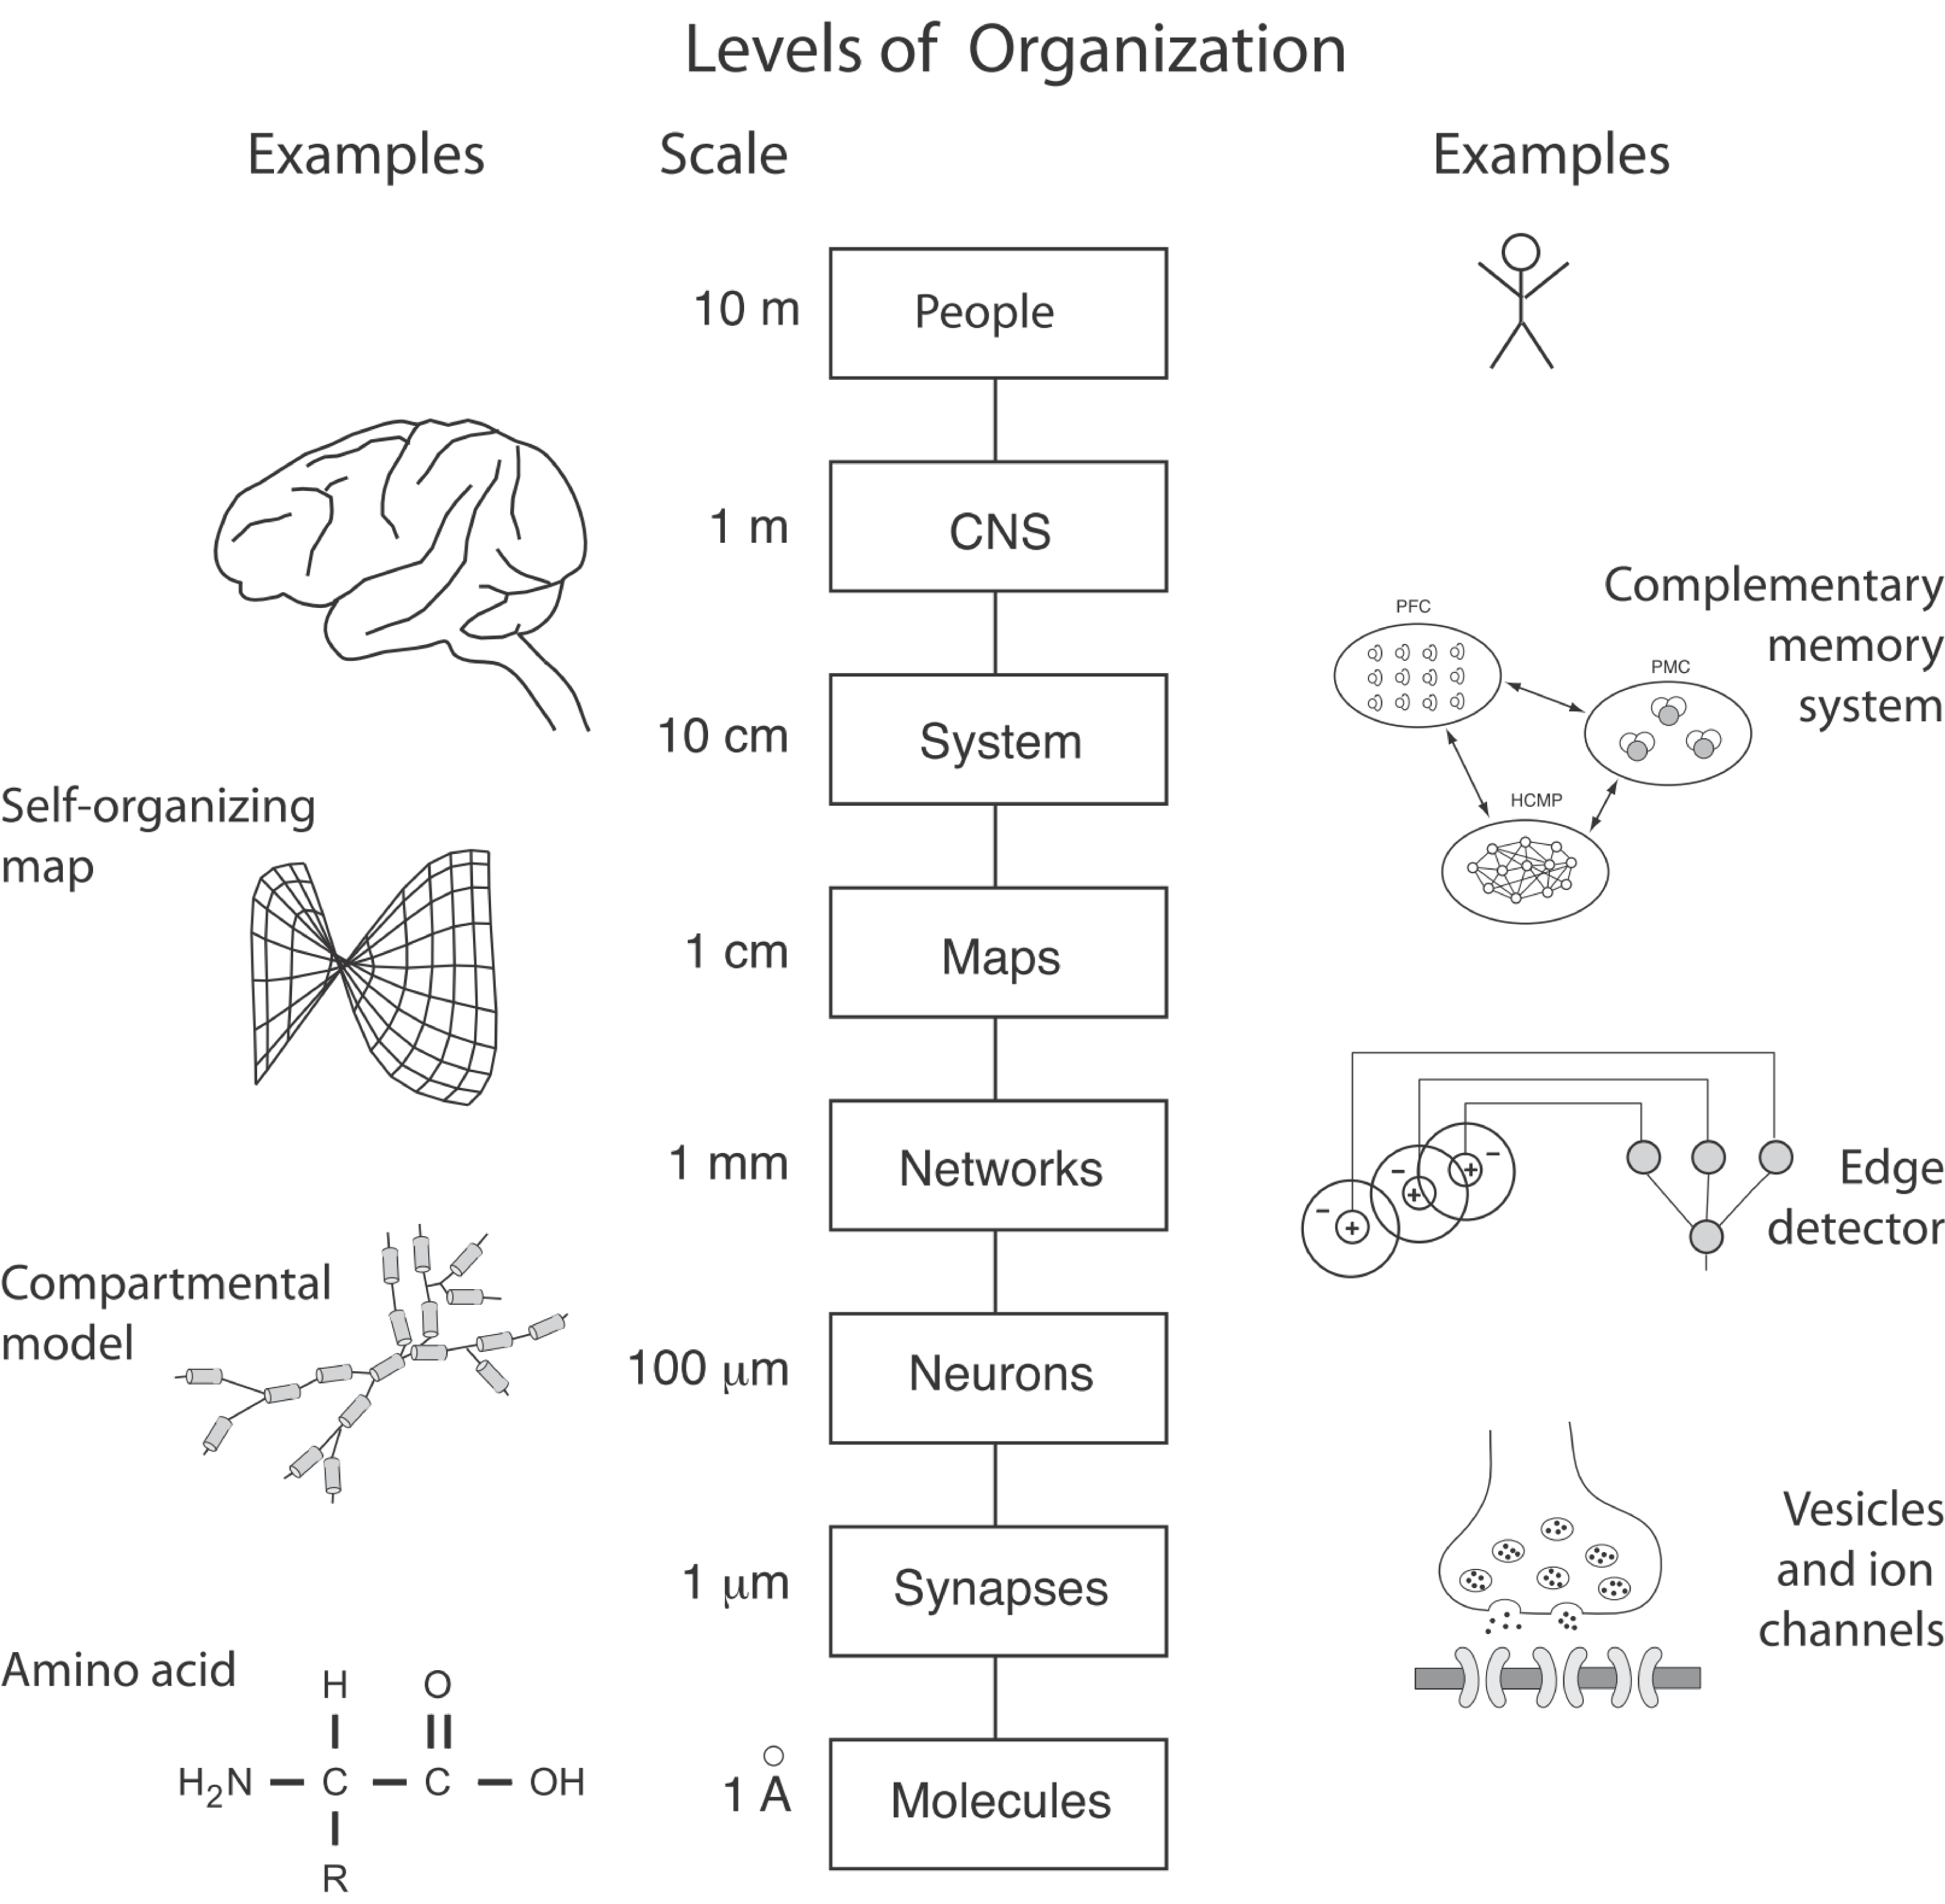
\includegraphics[width=\columnwidth]{graphics/levels.png}
		\caption[The levels of organisation in the \ac{CNS}]{\textbf{The levels of organisation in the \ac{CNS}}. Each level can be modelled in more or less detailed as required. (used with permission of Prof. Trappenberg \cite{Trappenberg2009}).} 
		\label{fig:levels}
\end{figure}


According to the diagram in figure \ref{fig:levels} and the scales, the research reported in this thesis covers the ``Neurons'' level. 

\subsection{Lapicque's integrate-and-fire model}

One of the earliest models of a neuron was in 1907 by Louis Lapicque. Lapicque's model describes what he observed in experiments with frogs. The mechanisms responsible for neuronal action potentials were unknown, and thus Lapicque's model was very simple. Despite the lack of detailed knowledge, Lapicque's model is still the basis of many models that are widely used today \cite{Abbott1999}. Lapicque postulated that nerve membranes were semi-permeable, polarisable membranes and could therefore be modelled as a capacitor with a leak. He compared the data obtained from his frog experiments with both an RC-circuit (a circuit with a resistor and a capacitor in parallel, fig \ref{fig:lapicque}) and a heuristic law of excitability \cite{Brunel2007}.

\begin{figure}[H]
	\centering
		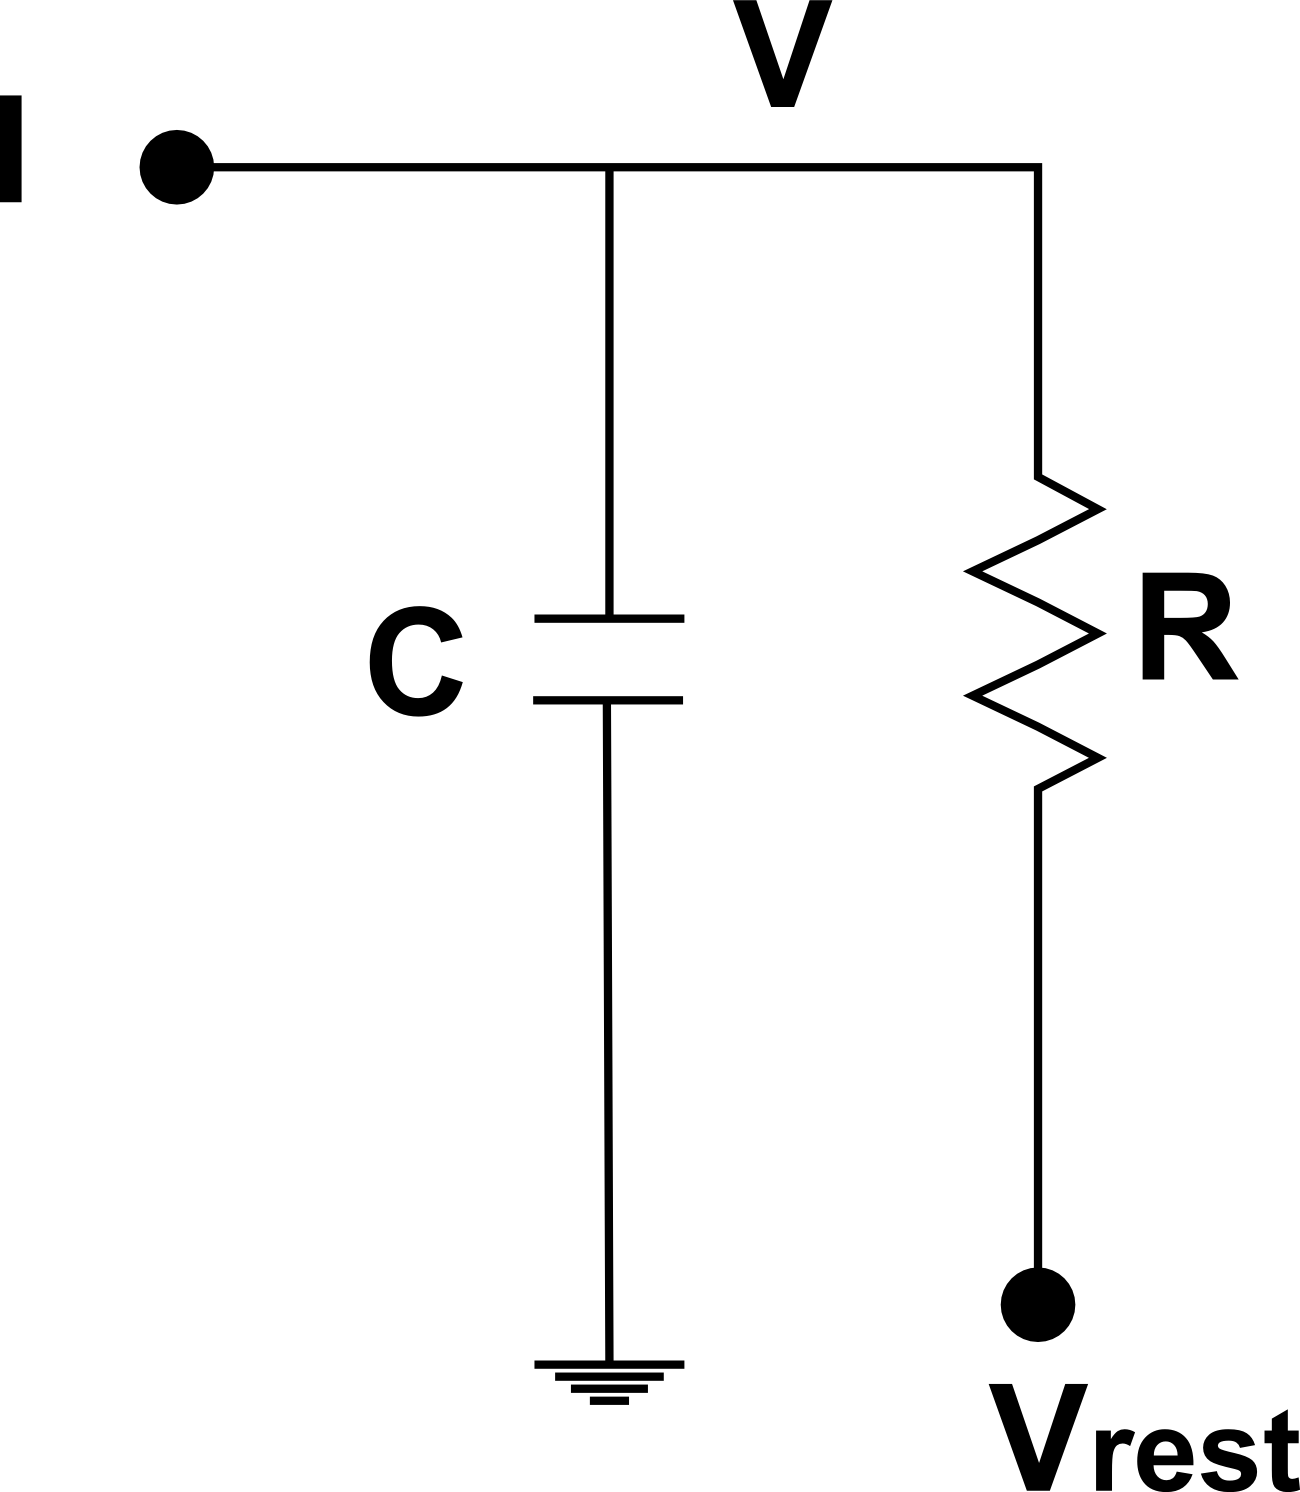
\includegraphics[width=4cm]{graphics/lapicque.png}
		\caption[Lapicque's model]{\textbf{Lapicque's model.} Lapicque's model was based on an RC-circuit. C is the membrane capacitance, R is the membrane resistance, V is the membrane potential, $V_{rest}$ is the resting membrane potential and I is an injected current.}
		\label{fig:lapicque}
\end{figure}

This model can be expressed as the time derivative of the law of capacitance, $Q=CV$. A neuron represented in time would thus be:

\begin{equation}
\label{eq:lapicque}
I(t)=C_{m}\frac{dV_{m}(t)}{dt}
\end{equation}

\subsection{The leaky integrate-and-fire-model}

An improvement on the integrate-and-fire model is the ``leaky integrate-and-fire'' model. This model adds a leak resistance in parallel to the capacitance, which reflects the diffusion of ions through the cell membrane. This model neuron will only fire when the excitatory input is strong enough to overcome the leak (\ref{eq:leaky}).

\begin{equation}
\label{eq:leaky}
I(t)-\frac{V_{m}(t)}{R_{m}}=C_{m}\frac{dV_{m}(t)}{dt}
\end{equation}

The leaky integrate-and-fire model is also known as the ``passive integrate-and-fire'' model because in its simplistic form, all active membrane conductances and synaptic inputs are ignored and the entire membrane is modelled as a single passive leakage term \cite{Dayan2001} %page 164

Semi-permeability of cell membranes is the result of embedded ion channels and pumps. These channels and pumps allow different concentrations of ions to be maintained inside and outside the cell which, in turn, result in an electrical potential existing across the membrane \cite{Sterratt2011}. 

%note {If we don't care about the biomechanical mechanisms, but just want to describe the action potential as a standard pulse then }
\subsection{Hodgkin-Huxley Model}
\label{sec:hogkin_huxley_model}

In 1952 Hodgkin and Huxley described the membrane current in the squid giant axon as an electrical circuit (Fig. \ref{fig:circuit}) and produced a set of differential equations which modelled the ionic currents across the membrane of excitable cells. These equations are still in use today \cite{Hodgkin1952, Hodgkin1952a, Hodgkin1952b, Hodgkin1952c, Hodgkin1952d}. Their work was a breakthrough in the understanding of nerve excitation. The equations in these papers provided only for potassium ion, sodium ion and leak currents. However, the same equations can be used to expand the model to include other currents and as such still serve as the basis of most neuronal models. These models are also known as conductance-based models.

\begin{figure}[H]
	\centering
		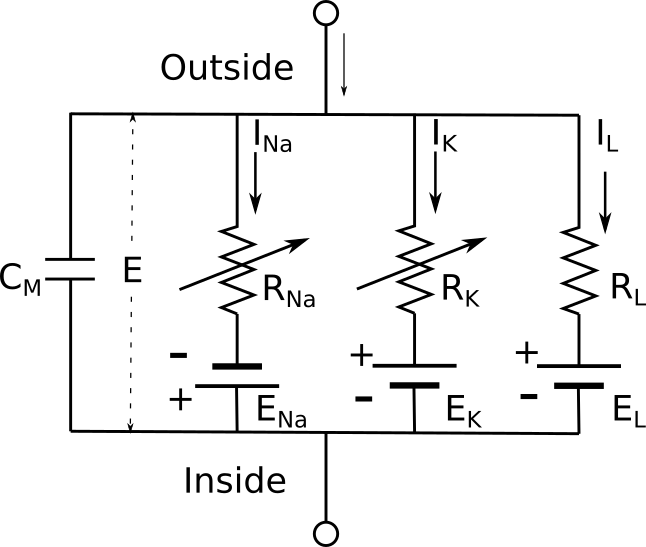
\includegraphics[width=\columnwidth]{graphics/HodgkinHuxley.png}
		\caption[The membrane as an electrical circuit.]{\textbf{The membrane as an electrical circuit.} Hodgkin-Huxey described the membrane current in the squid giant axon as an electrical circuit. \cite{Hodgkin1952a}}
		\label{fig:circuit}
\end{figure}

%See CNN2a.pdf
%Beckerman2005 page 467
Action potentials are the result of joint action by fast-acting sodium channels and delayed-acting potassium channels \cite{Beckerman2005}.
Sodium (Na\textsuperscript{+}) channels can be in any of a number of states, depending on the channel's internal activation, inactivation or deactivation state and whether it is open or closed. The channel only allows Na\textsuperscript{+} to move through when it is both open and activated. Potassium channels have only two states, open or closed. The channels responsible for ``leak currents'' are open all the time and are mostly responsible for the resting membrane potential. The leak current is mostly made up of chloride ions \cite{Hodgkin1952a}. The sodium and potassium channels are also ion specific. However, these channels are voltage dependent, meaning that the probability of them being open or closed depends on the voltage across the cell membrane. In figure \ref{fig:circuit}, this voltage dependency is indicated by the symbol for a variable resistor (a resistor with an arrow through it). 

The mathematical equation for the electrical circuit is given by:

\begin{equation}
\label{eq:membrane_current}
I=C_{M}\frac{dV_{m}}{dt} + I_{int}
\end{equation}

where: 

$I$ is the total membrane current.

$C$ is the membrane capacitance.

$I_{int}$ the sum of the intrinsic and modulatory ionic currents.

$V_{m}$ is the membrane potential.

$t$ is time.



Voltage gated sodium channels in the cell membrane are responsible for the depolarising phase that eventually leads to action potentials. Voltage-gated potassium channels, on the other hand, are crucial for hyperpolarisation to return the cell to a resting state \cite{Lodish2000}.

%\cite{Buchholtz1992}

In the Hodgkin-Huxley model, each of the voltage gated sodium channels is assumed to have two gates: the 'm' and the 'h' gate. For the channel to be open, both gates have to be in an open state. The channel is in a deactivated state if the m channel is closed or an inactivated state if the h channel is closed. When both gates are open the gate is activated. The states of the gates are described in the Hodgkin-Huxley equations by:

\begin{equation}
\label{eq:activationcurve}
I = g_{ion}m^{p}_{ion}h^{q}_{ion}(V - E_{ion})
\end{equation}

As given, this equation (Eq: \ref{eq:activationcurve}) is generic and can be used for all ionic conductances. The maximal conductance of the channel is $g$, while $m$ and $h$ are the fractions of activation and inactivation gates in the open state, and $p$ and $q$ are the number of independent gates per channel. $V$ is the displacement of the membrane potential from its resting value and $E_{ion}$ is the reversal potential that corresponds to the specific ion \cite{Buchholtz1992, Hodgkin1952a, Willms1999, Soto-Trevino2005}.

The Hodgkin-Huxley model of an excitable cell is summarised in four differential equations:

\begin{equation}
\label{eq:HH}
I = C_{m}\frac{d V_{m}}{dt}  + {g}_{K}n^{4}(V_{m} - V_{K}) + {g}_{Na}m^{3}h(V_m - V_{Na}) + g_{l}(V_{m} - V_{l})
\end{equation}
\begin{equation}
\frac{dn}{dt} = \frac{-(n-n_{\infty}(V)) }{ \tau_{n}(V)}
\end{equation}
\begin{equation}
\frac{dm}{dt} = \frac{-(m-m_{\infty}(V)) }{ \tau_{m}(V)}
\end{equation}
\begin{equation}
\frac{dh}{dt} = \frac{-(h-h_{\infty}(V)) }{ \tau_{h}(V)}
\end{equation}

where:

$I$ is the total membrane current,

$C_{m}$ is the membrane capacitance,

$V_{m}$ is the membrane potential,

$t$ is time,

$g_{K}$, $g_{Na}$, $g_{l}$ are the ionic conductances for potassium (K), sodium (Na) and leakage (l) respectively. 

$\alpha$ and $\beta$ are rate constants that vary with voltage but not with time.

The reversal potential for each current can be calculated by using the Nernst equation (Eq. \ref{eq:Nernst})


\begin{equation}
\label{eq:Nernst}
E = \frac{RT}{zF}ln\frac{[ion]_{extracellular}}{[ion]_{intracellular}}
\end{equation}

where:

$E$ is the membrane potential in volts,

$R$ is the ideal gas constant of 8.3144621 $\frac{J}{mol K}$,

$T$ is the temperature in Kelvin,

$z$ is valence of the ion,

$F$ is Faraday's constant for which the currently accepted value is $9.64853399 x 10^{4}C mol^{-1}$,

and $[ion]_{extracellular}$ and $[ion]_{intracellular}$ are the intra- and extracellular ion concentrations respectively in moles per cubic meter.

However, to take into account all of the ions that are permeant through a cell membrane the Goldman-Hodgkin-Katz equation is used:

\begin{equation}\label{eq:GHK}
E_{m} = \frac{RT}{F}ln\frac{P_{Na^{+}}[Na^{+}]_{out}+P_{K^{+}}[K^{+}]_{out}+P_{Cl^{-}}[Cl^{-}] _{in}}{P_{Na^{+}}[Na^{+}]_{in}+P_{K^{+}}[K^{+}]_{in}+P_{Cl^{-}}[Cl^{-}]_{out}}
\end{equation}

Various researchers have based models on the Hodgkin-Huxley model to simplify or adapt the models for specific purposes. Some well-known models the Morris-Lecar \cite{Morris1981} model, FitzHugh-Nagumo \cite{Fitzhugh1961, Nagumo1962} model and the Hindmarsh-Rose model.

\subsection{Multi-compartmental models}
The aforementioned models describe the membrane potential over an entire neuron with a single variable. Membrane and morphological properties vary along the length of an axon resulting in varying membrane potentials over the surface of the neuron \cite{Dayan2001, Sterratt2011}. The effect of the varying membrane potentials and associated complexities can be reproduced in models by considering a neuron as several connected compartments. Each compartment can be simulated by a Hodgkin-Huxley type model (or any other appropriate type of model) with the compartments connected via conductances \cite{Izhikevich2007}\note{page 43}
\note{Dayan, page219}

\subsection{Existing pyloric \ac{CPG} neuron models from literature}
Table \ref{tab:models} lists models of pyloric \ac{CPG} neurons from crustacean that can be found in literature. The table shows the journal reference, the number of neurons that were modelled and the equations that were used. The model with the most number of neurons was the Gutierrez model. The purpose of this model was to illustrate circuit switching using network motifs that are found in the \ac{STG} network. The neurons were modelled as single compartments and using the Morris-Lecar two-dimensional reduced excitation model. Neurons in this model do not reflect physiological properties of the biological neurons (eg. \ac{PD} and \ac{LP} are modelled using the same equations in anti-phase) \cite{Gutierrez2013}.

\begin{table}[H]
	\centering
	\footnotesize
	\caption[\ac{STG} model list]{\textbf{\ac{STG} model list.} A list of published \ac{STG} models by various researchers, showing the number of neurons simulated and the equations used in the model}
	\label{tab:models}
	\begin{tabular}{l l c l l}	
		\textbf{Paper} & \textbf{Neurons} &  \textbf{\#}  & Equations & \textbf{Notes}\\ \hline
		Buchholz 1992 \cite{Buchholtz1992} & LP & 1 & Hodgkin-Huxley & \\
		Epstein 1990 \cite{Epstein1990} & unidentified & 1 & Hodgkin-Huxley & Three models of  \\
		& & & & individual neurons\\
		Golowasch 1992 \cite{Golowasch1992} & LP & 1 & Hodgkin-Huxley & \\ 
		Prinz 2003 \cite{Prinz2003a} & PD & 1 & Hodgkin-Huxley & Database of 1.7 \\
		& & & & million \\
		& & & & single-compartment \\
		& & & & models\\
		
		Abbot 1991 \cite{Abbott1991} & AB, PD & 2 &  FitzHugh-Nagumo & \\
		Golowasch 1999 \cite{Golowasch1999a} & AB/PD, PY & 2 & Hodgkin-Huxley & AB/PD modelled as \\
		& & & & one\\
		Soto-Trevino & AB, PD & 2 & Hodgkin-Huxley & \\
		2005 \cite{Soto-Trevino2005} & & & & \\
		
		Hartline 1979 \cite{Hartline1979} & AB/PD, & 3 &  & AB/PD modelled as\\
		&  LP, PY & & & one\\
		Warshaw 1976 \cite{Warshaw1976} & LP, PD, PY,& 5 & & \\
		& VD, IC & & & \\
		
		Gutierrez 2013 \cite{Gutierrez2013} & IC, LP, & 5 & Morris-Lecar & Illustrating circuit \\
		& LG, PD, Int1 & & & switching\\
	\end{tabular}
\end{table}


Very early models from the Hartline laboratory \cite{Hartline1979, Warshaw1976} also included up to five neurons. These models used Morris-Lecar type equations and were implemented in SNAX, a language for interactive neuronal modelling  and  data  processing \cite{Hartline1976}. SNAX does not seem to be available any more and unfortunately the old journal articles could not be obtained to learn more about the language. 


Note that the Morris-Lecar model is a simplified version of the Hodgkin-Huxley model which, for example, does not capture the details of spiking activity in neurons.  With such a configuration it is not possible to model the differential modulation which occurs when \ac{STG} neurons are exposed to \ac{DA}.

\subsection{How models are created}
The models discussed are expressed as differential equations. These systems are non-linear and cannot be solved analytically. It is possible, though, to use numeric methods. 

An interesting anecdote from the pen of Alan Hodgkin, makes us appreciate the general availability of computers today:

\textit{``Finally there was the difficulty of computing the action potentials from the equations which we had developed. We had settled all the equations and constants by March 1951 and hoped to get these solved on the Cambridge University Computer. However, before anything could be done we learnt that the computer would be off the air for 6 months or so while it underwent a major modification. Andrew Huxley got us out of that difficulty by solving the differential equations numerically using a hand-operated Brunsviga. The propagated action potential took about three weeks to complete and must have been an enormous labour for Andrew. But it was exciting to see it come out with the right shape and velocity and we began to feel that we had not wasted the many months that we had spent in analysing records.''} \cite{Hodgkin1976}

Using MATLAB$^{\copyright}$ on an i5 laptop with 6 gigabytes of RAM and a very simple implementation of the Hodgkin-Huxley model (Appendix \ref{app:HH}), it now takes approximately 0.194440 seconds to produce the graph (Fig. \ref{fig:hh_curve}) that took Andrew Huxley three weeks with the use of the Brunsviga calculator (Fig \ref{fig:brunsviga}).

\begin{figure}[H]
	\centering
		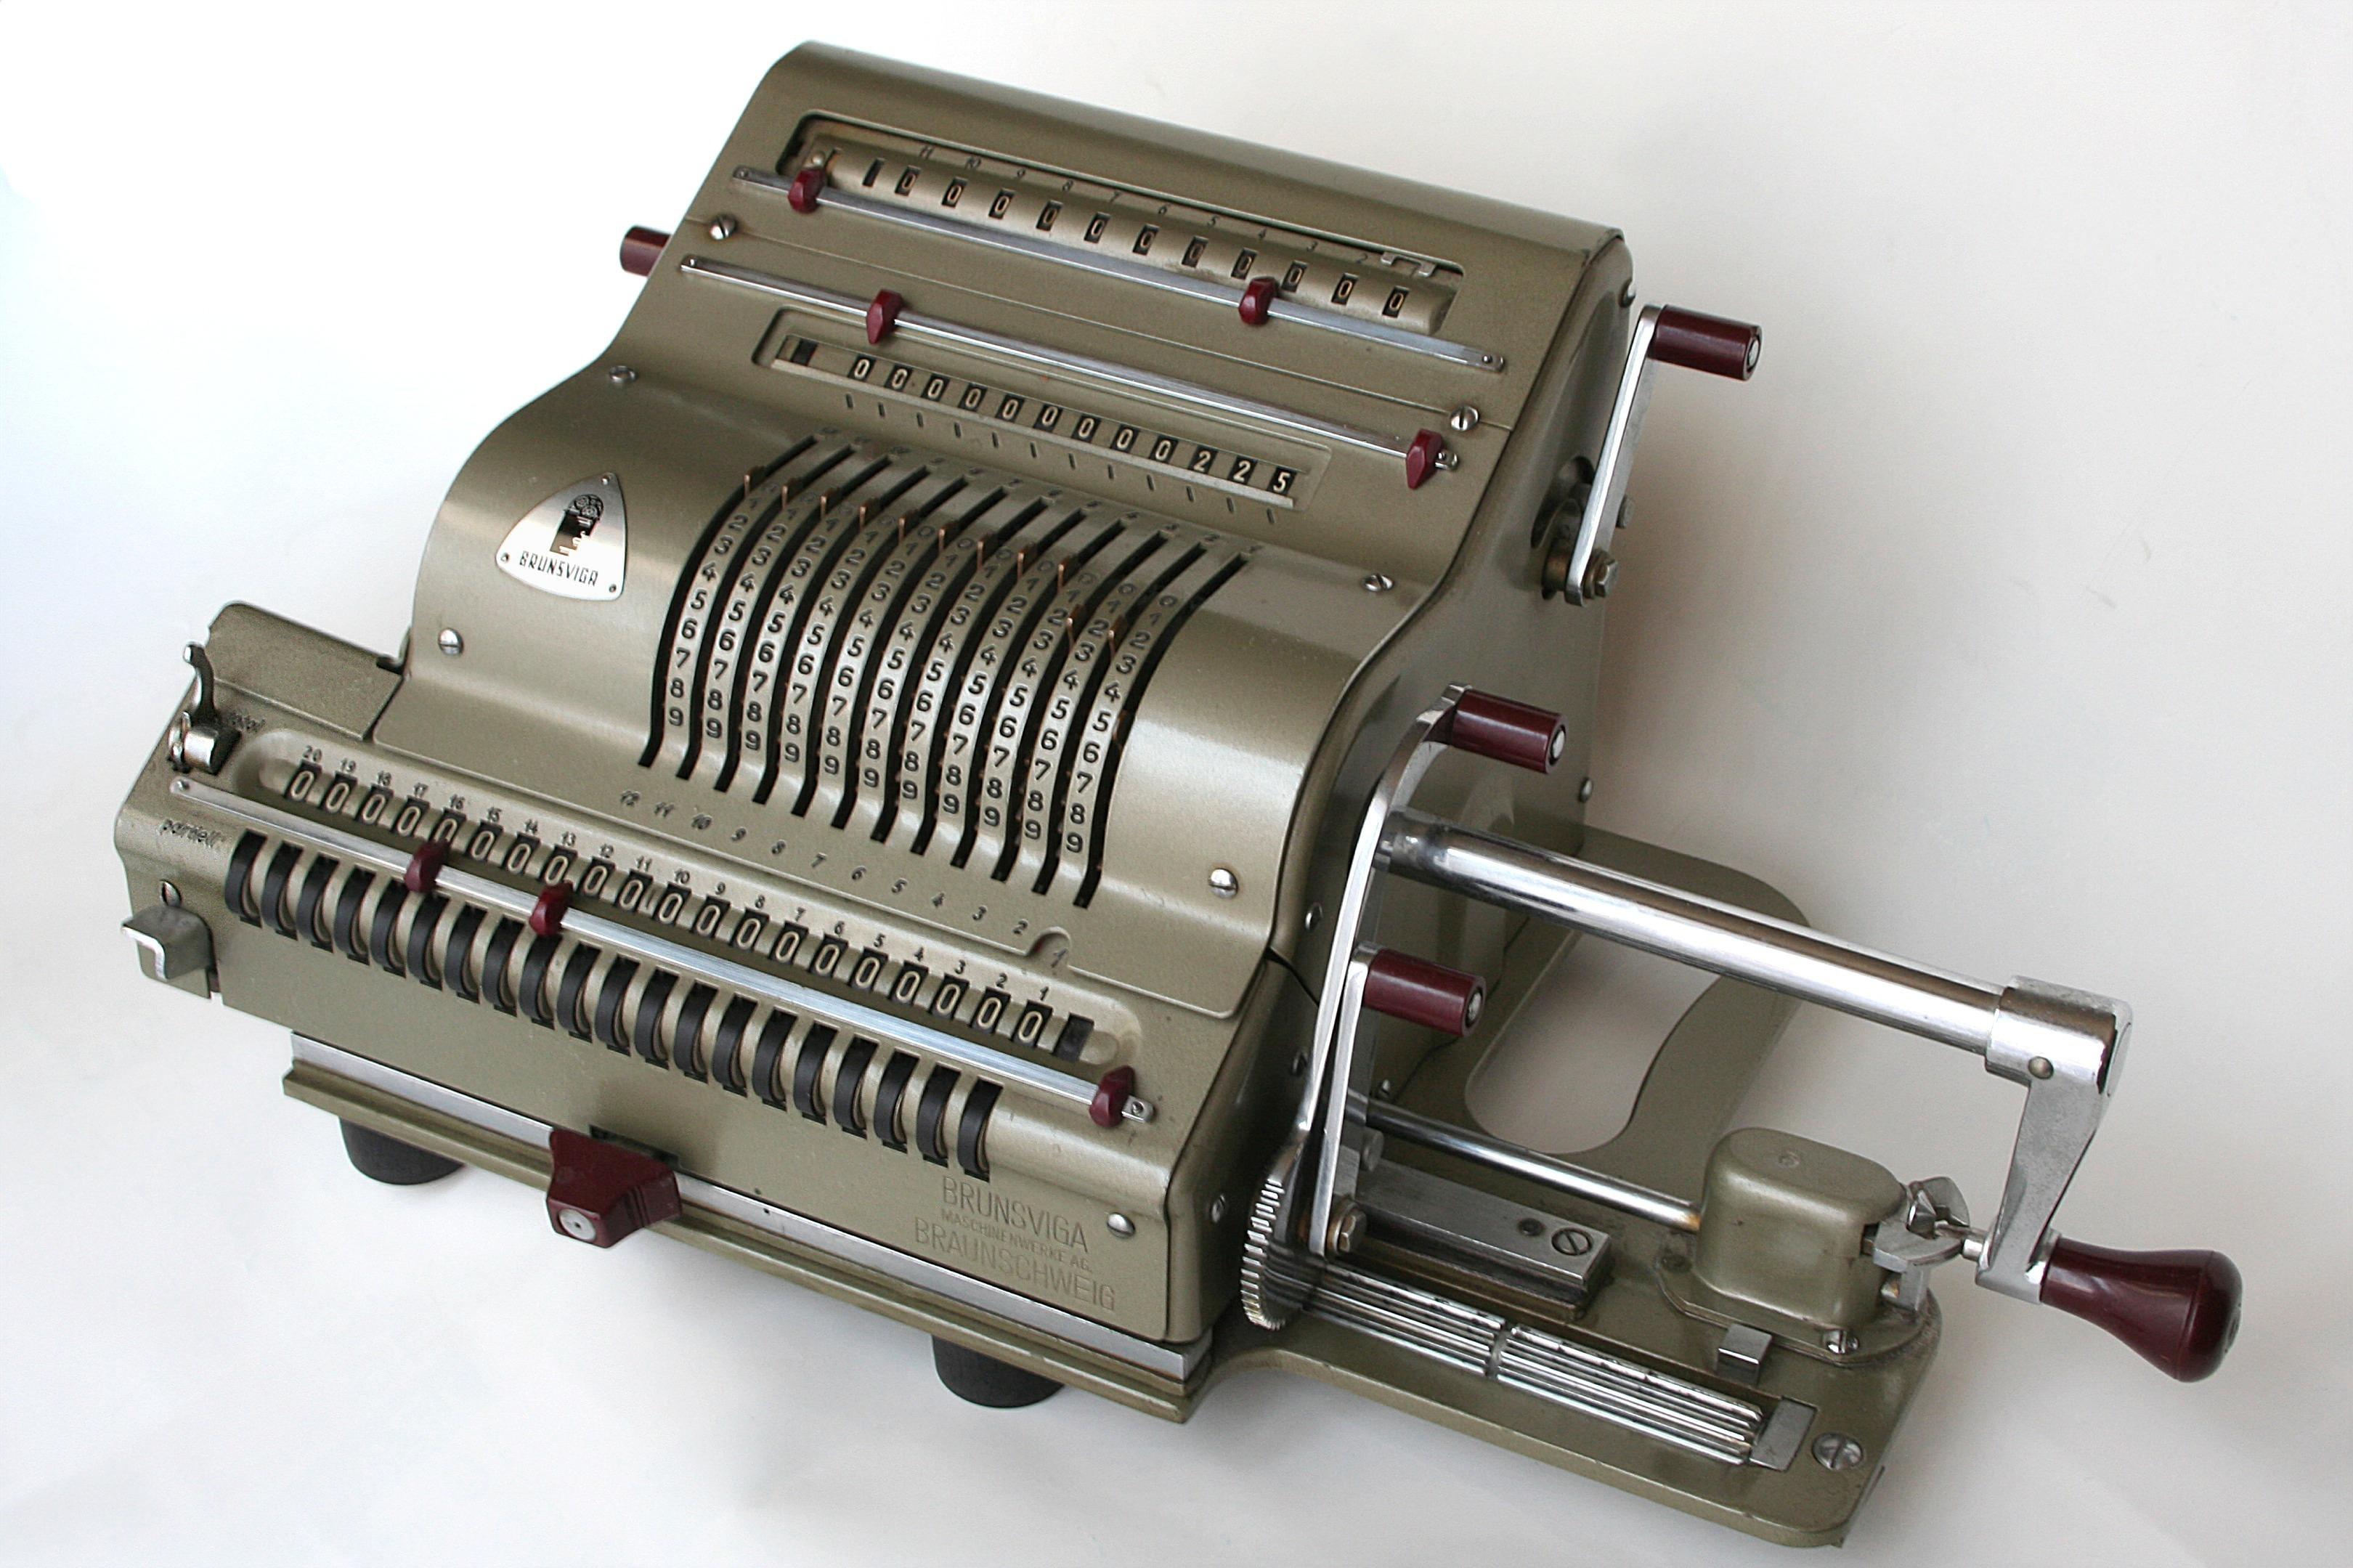
\includegraphics[width=9cm]{graphics/Brunsviga.jpg}
		\caption[A Brunsviga hand-operated calculator]{\textbf{A Brunsviga hand-operated calculator.} A Brunsviga hand-operated calculator such as was used by Andrew Huxley in 1951. (Image by Lothar Spurzem (Spurzem) [CC BY-SA 2.0 de, \url{http://creativecommons.org/licenses/by-sa/2.0/de/deed.en}], Wikimedia Commons)} 
		\label{fig:brunsviga}

		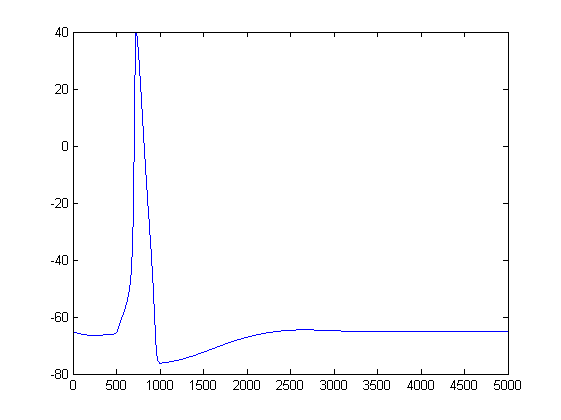
\includegraphics[width=9cm]{graphics/HH_curve.png}
		\caption[An action potential curve]{\textbf{An action potential curve}. A curve produced in 0.194440 seconds with the Hodgkin-Huxley equations using MATLAB$^{\copyright}$.} 
		\label{fig:hh_curve}
\end{figure}

By Lothar Spurzem (Spurzem) (Created by Spurzem.) [CC BY-SA 2.0 de (http://creativecommons.org/licenses/by-sa/2.0/de/deed.en)], Wikimedia Commons

In this day and age and for the purpose of this research it would not be unreasonable to take the availability and use of computers as a given. Thus, the history and details of numerical solvers will not be discussed but rather the software and choices of numerical solvers implemented in the software will be considered. Various numerical solvers are available and it is up to the researchers to select an appropriate solver based on the nature of the equations to be used.

With regards to software there are various commercial and open source packages available such as MATLAB from MathWorks$^{\copyright}$\footnote{\url{https://uk.mathworks.com/products/matlab/}}, GNU Octave\footnote{\url{https://gnu.org/software/octave/}} (an open source product, mostly compatible to MATLAB) and R\footnote{\url{http://www.r-project.org/}} which is also open source. 

There are also software available specifically for neuron simulation such as NEURON\footnote{\url{http://www.neuron.yale.edu/neuron/}} and the GENESIS\footnote{\url{http://genesis-sim.org/}} (GEneral NEural Simulation System) simulator. These simulators have built-in numerical solvers and in some cases the user might be offered a selection of solvers to choose from.

The stiffness of the equations of the selected model is an important determinant in the selection of the appropriate software and numerical solver to be used. ``Stiffness'' arises when one has to deal with more than one first-order differential equation where some dependent variables are changing based on two or more independent variables that have very different scales \cite{Press1992}.\note{page 734, section c16-6}

\note{Curtiss1952, ode45berkley}

In the case of the Hodgkin-Huxley model there are slow components and fast components. The equations are stiff because of the interactions between the membrane potential and the three conductance variables \cite{Chance1981}. Thus a numerical solver that can cope with this ``stiffness'' in the equations need to be selected.

Typically, for models derived from the Hodgkin-Huxley model, a fourth-order Runge-Kutta method with predictions is used (Runge-Kutta(4,5)). Predictions are made with an adaptive step-size algorithm.

Another interesting result from the Hodgkin-Huxley studies is the fact that neurons emerged as dynamical systems and can therefore be studied as such. 

The Hodgkin-Huxley model is a four-dimensional dynamical system of ordinary differential equations governing the evolution of four state variables, $V$, $n$, $m$ and $h$ \cite{Izhikevich2007}. The model exhibits bi-stability between equilibrium and limit cycle attractors. If a constant current is injected that is below the threshold where tonic firing takes place, the system will go to a fixed point. When a higher current is injected, the fixed point becomes unstable and solutions converge to a stable periodic trajectory which is known as a limit cycle (figure \ref{fig:limitcycle}) \cite{Fitzhugh1960, Meunier2001}.

\begin{figure}[H]
	\centering
		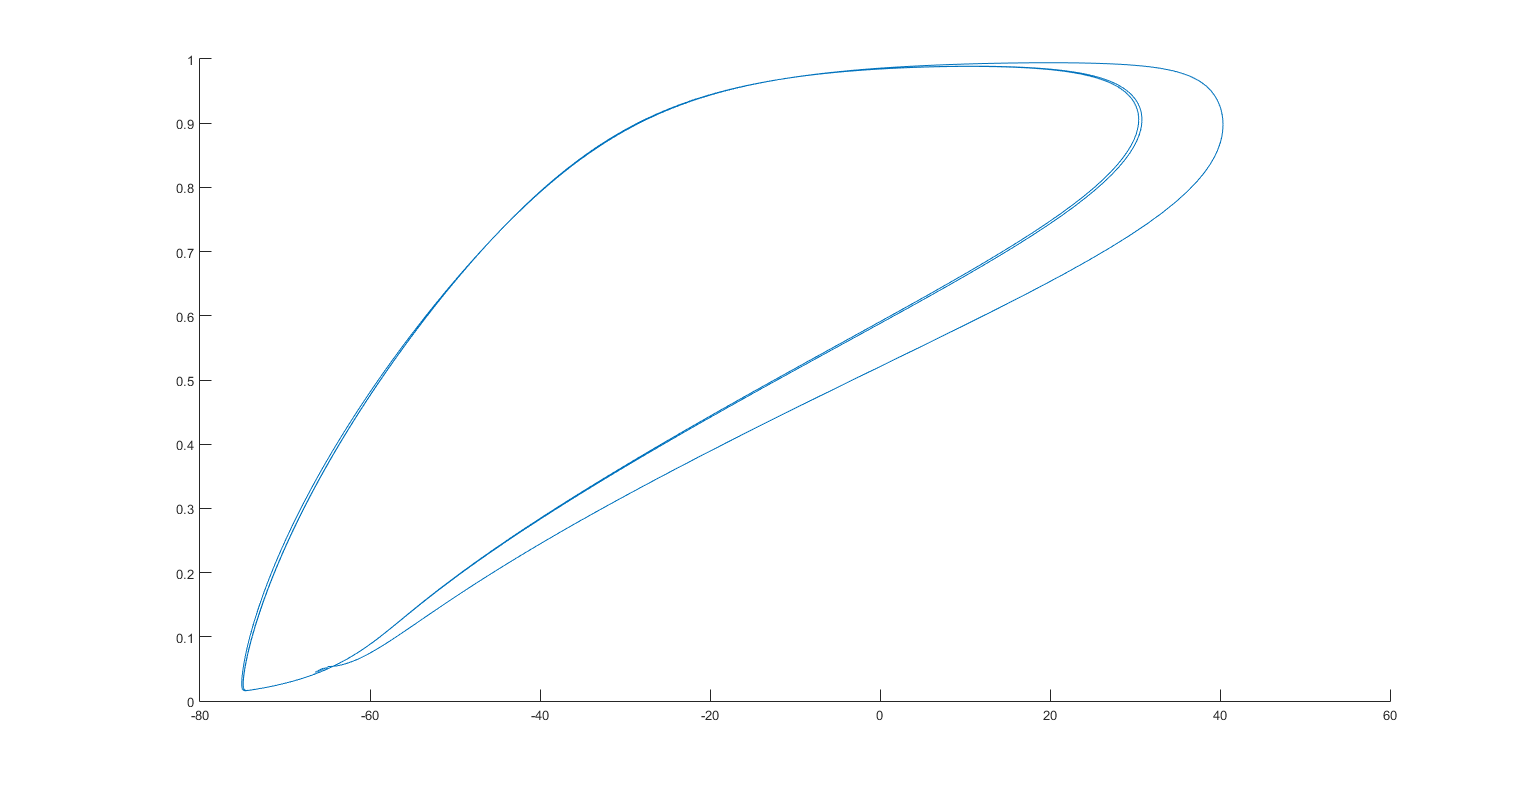
\includegraphics[width=\columnwidth]{graphics/limitcycle.png}
		\caption[Limit cycle]{\textbf{Limit cycle.} Using the model from appendix \ref{app:HH}, this limit cycle was produced by plotting $m$ against $v$.}
		\label{fig:limitcycle}
\end{figure}

\note{\url{https://books.google.co.uk/books?id=w8Nxnr47690C&pg=PA371&lpg=PA371&dq=hodgkin+huxley+dynamical+system+fixed+attractor&source=bl&ots=akbF-Z3f6E&sig=kELxQwL79QkxHeMkERwcmoUbPaQ&hl=en&sa=X&ei=uMIvVfnyBMHiaMGdgPAB&ved=0CDwQ6AEwAw#v=onepage&q=hodgkin\%20huxley\%20dynamical\%20system\%20fixed\%20attractor&f=false}}
\note{system in permanent flux - Belousov Zhabotinsky reaction
	
	when the neuron is spiking you need a limit cycle attractor and not a fixed point attractor
	Describe that if you have these equations then how does the system works . say something about the equilibrium point being stable or unstable . When it is stable it is a fixed point attractor when not then talk about other attractors such as limit cycles such as strange (chaotic) attractor which won't discuss.
	Paper not finished because did not do enough temporal averaging
}
\note{
	http://stsutsui.com/projects/hh.html}
\subsection{Finding Parameters}
A vital aspect of computational modelling is finding appropriate values for model parameters. The values could be based on measurements taken during experiments, but are often estimates or even complete guesses \cite{Sterratt2011}.

In the Hodgkin-Huxley based models there is requirement for conductance values ($g$). These values are usually experimentally measured but are highly variable \cite{Golowasch1999,Zhao2012}. Prinz, for instance, computationally generated 20,250,000 model networks from combinations of a three neuron circuit varying the synaptic strengths and neuron properties. The circuit was based on the pyloric \ac{CPG} of \species{H. americanus}. Of these model  4,047,375, 20\%, produced pyloric-like behaviour, confirming that similar network activity can be produced from disparate circuit parameters \cite{Prinz2004a}.

It has also been shown, in the pyloric neurons of the crustacean \ac{STG}, that ionic conductances are expressed in a correlated fashion \cite{Temporal2012} and that these correlations contribute to the invariance of neuron activity and spiking frequencies \cite{Zhao2012}. 
\note{\cite{Hodgkin1952d,Soto-Trevino2005}}
\note{Bumbaugh-thesis}
\note{stiffness: mascagni_sherman.pdf page 32}

% words 6250

This background section is by no means comprehensive. Each of the sections covered justifies research in its own right and is the subject of several books, articles and research groups. The nature of this research is such that it requires an interdisciplinary approach. Continuous progress in technology also means that knowledge and skills of all the contributory fields need to be kept up to date. For instance, progress made in optogenetics might soon make it an option for recording neural activity in the \ac{STG}. The background given, will hopefully serve to put the research question and the technical requirements into perspective.

%Background
	\chapter{Methods and Materials}
\label{chap:methodsAndMaterials}
\acresetall
\section{Introduction}
\label{sec:introduction}
The planar arrangement of the cell bodies of the crustacean \ac{STG} makes the neural system particularly well suited for the recording of single or multiple neurons using electrophysiology or voltage-sensitive dye imaging. To be able to compare the output of a model system to the output of a complete biological neural system, but with the insight into the contribution of individual neurons that comprise the system, would be invaluable. Capturing such neural activity from the \ac{STG} requires that the \ac{STNS} be dissected from a live crab. The methods for dissecting the crustacean \ac{STNS} are quite mature. 

The use of \ac{VSD} on the \ac{STG} has only been done since 2010 in the Newcastle University crab lab (which was moved to Keele University in August 2014) by Prof Peter Andras in collaboration with Dr Wolfgang Stein. The Newcastle University crab lab was also the only laboratory investigating and developing the techniques for using \ac{VSD} on the crustacean \ac{STG}. In 2012 Dr Wolfgang Stein set up a laboratory at Illinois State University which now also investigate the use of \acp{VSD} on the \ac{STG} and other ganglia of the \ac{STNS}.

Because the use of \ac{VSD} for research into the neural activity of the \ac{STG} is still relatively new, the methods for the analysis of the data, especially for the use of verifying computational models of the \ac{STG}, were inadequate or non-existing when this research project started. This research contributes in this respect by providing new methods for recording of the complete \ac{STG} and for the analysis of the recorded data.

In this chapter the methods and materials adopted and developed are described. These methods and materials include obtaining and keeping crabs, dissections, electrophysiology, the application of \acp{VSD} both intracellularly and bath-applied, the methods developed for analysing the data and lastly, the building and analysis of a computational model.

\section{Obtaining and Keeping Crabs for Dissection}
\label{sec:obtaining_crabs}

For this research \textit{Cancer pagurus}, also known as the \textbf{edible crab} or \textbf{brown crab}, was used. These crabs are found in the North Sea and North Atlantic Ocean.

Crabs were obtained from suppliers at North Shields Fish Quay and some were obtained from Dove Marine Laboratory in Cullercoats\footnote{Dove Marine Laboratory, Newcastle University (\url{http://www.ncl.ac.uk/marine/facilities/dove/})}. Initially the purchased crabs were then kept at the Ridley Building (School of Biology, Newcastle University) but later on the crabs were kept in the crab lab in two 60 litre aquariums in artificial sea water. The water was filtered and chilled to 14 degrees Celsius.

Crabs with a carapace width of 12 to 15 cm were selected. Both male and female crabs were used.

\section{Dissection}
\label{sec:dissection}

The dissection of the brown crab (\species{Cancer pagurus}) is done in two parts: the gross and fine dissection. The methods are the same as for other crabs, such as the Jonah crab (\species{Cancer borealis}) which is used in many other labs. During the gross dissection the carapace is opened up with rongeurs and the stomach is removed. The stomach is opened by making an incision from the oesophagus (anterior) to the pylorus (posterior). The stomach is then pinned down in a dish lined with black Sylgard, with the inside of the stomach to the bottom and covered with \species{Cancer pagurus} saline (see table~\ref{tab:saline}). All tissue on the dorsal side of the stomach is removed to expose the \ac{STNS}.

During the fine dissection the \ac{STNS} is removed from the stomach using a microscope and microdissection tools, and pinned into a Sylgard lined petri dish. The nerves are cleared of all tissue. If intra-cellular or voltage sensitive dye recordings are to be made, the \ac{STG} has to be de-sheathed.

A detailed description of the gross and fine dissections are provided in Appendix \ref{app:dissection}, and an excellent video of the procedures is available on-line in the Journal of Visualized Experiments (JOVE) \cite{Gutierrez2009}.

\section{Electrophysiology}
\label{sec:electrophysiology}
Extracellular recordings of neurons in the \ac{STNS} are made by pinning out the deafferented \ac{STNS} in a Sylgard coated petri dish. A petroleum jelly well is made over the nerve of interest. To record the pyloric rhythm, the well is best made over the \ac{dvn} and/or the \acp{lvn}.

Using a differential amplifier such as the A-M Systems Model 1700 \footnote{https://www.a-msystems.com/s-129-differential-ac-amplifier-model-1700.aspx}, one electrode is placed inside the well and the other outside the well. The output from the differential amplifier is fed into a DAQ (data acquisition system) such as the CED 1401 Micro 3\footnote{http://www.ced.co.uk/2pl01u.shtml}. The DAQ connects to a computer where software such as Spike2\footnote{http://www.ced.co.uk/pru.shtml} or WinEDR\footnote{http://spider.science.strath.ac.uk/sipbs/showPage.php?page\=software\_winEDR} displays and records the activity measures over the electrodes.

Intra-cellular recordings are made using an intra-cellular amplifier such as the AxoClamp 900A Amplifier\footnote{http://www.moleculardevices.com/systems/conventional-patch-clamp/axoclamp-900a-microelectrode-amplifier}, made by Molecular Devices. The intra-cellular amplifier has a head stage into which a glass electrode is placed. Micro glass electrodes are pulled from glass capillaries using a puller such as the M-97 Flaming/Brown Micropipette Puller\footnote{http://www.sutter.com/MICROPIPETTE/p-97.html}.

The head stage is fitted to a micro-manipulator such as the Scientifica Patchstar Micro-manipulator\footnote{http://www.scientifica.uk.com/products/patchstar-micromanipulator}  that has an electronic movement resolution of 20 nm. Using the manipulator, the glass electrode is positioned above a neuron. The electrode is then lowered to just touch the cell membrane of the neuron. Using the intra-cellular amplifier software or an oscilloscope it is possible to see when the electrode touches the neurons as the measured voltage will suddenly drop. The electrode is then slowly lowered, using the manipulator, while simultaneously ``buzzing''. Buzz is a function of the intra-cellular amplifier which drives a short, large current oscillation through the electrode. These oscillations force the electrode into the cell membrane. As soon as the electrode breaks into the cell membrane, a typical intra-cellular wave form will appear on the oscilloscope/screen.

To keep the temperature of the preparation constant it has to be perfused. Perfusion is accomplished by using a pump to suck out the saline that covers the preparation in the Petri dish at the same time as feeding fresh cold saline into the dish. The temperature of the saline is maintained by running it over a Peltier device\footnote{http://stg.rutgers.edu/resources/Peltiers.pdf}. The inlet and outlet are placed as close to the \ac{STG} as possible to insure the \ac{STG} itself is kept at the required temperature which is between 10 and 15 degrees Celsius.

If neurotransmitters are to be applied to the preparation, a large well is made around the \ac{STG} to restrict application of the neurotransmitter to the \ac{STG} neurons. The perfusion inlet and outlet are placed inside the well. It is therefore important to make sure that the well is intact and has no leaks.

Figure \ref{fig:prep} shows a deafferented \ac{STNS} pinned and desheathed in a Petri dish. There are three wells placed over the \ac{dvn} and \ac{lvn} with extracellular electrodes. The large well in the centre around the \ac{STG} is used for perfusing the \ac{STG} with either saline or a dopamine solution.


\begin{figure}[H]
	\centering
		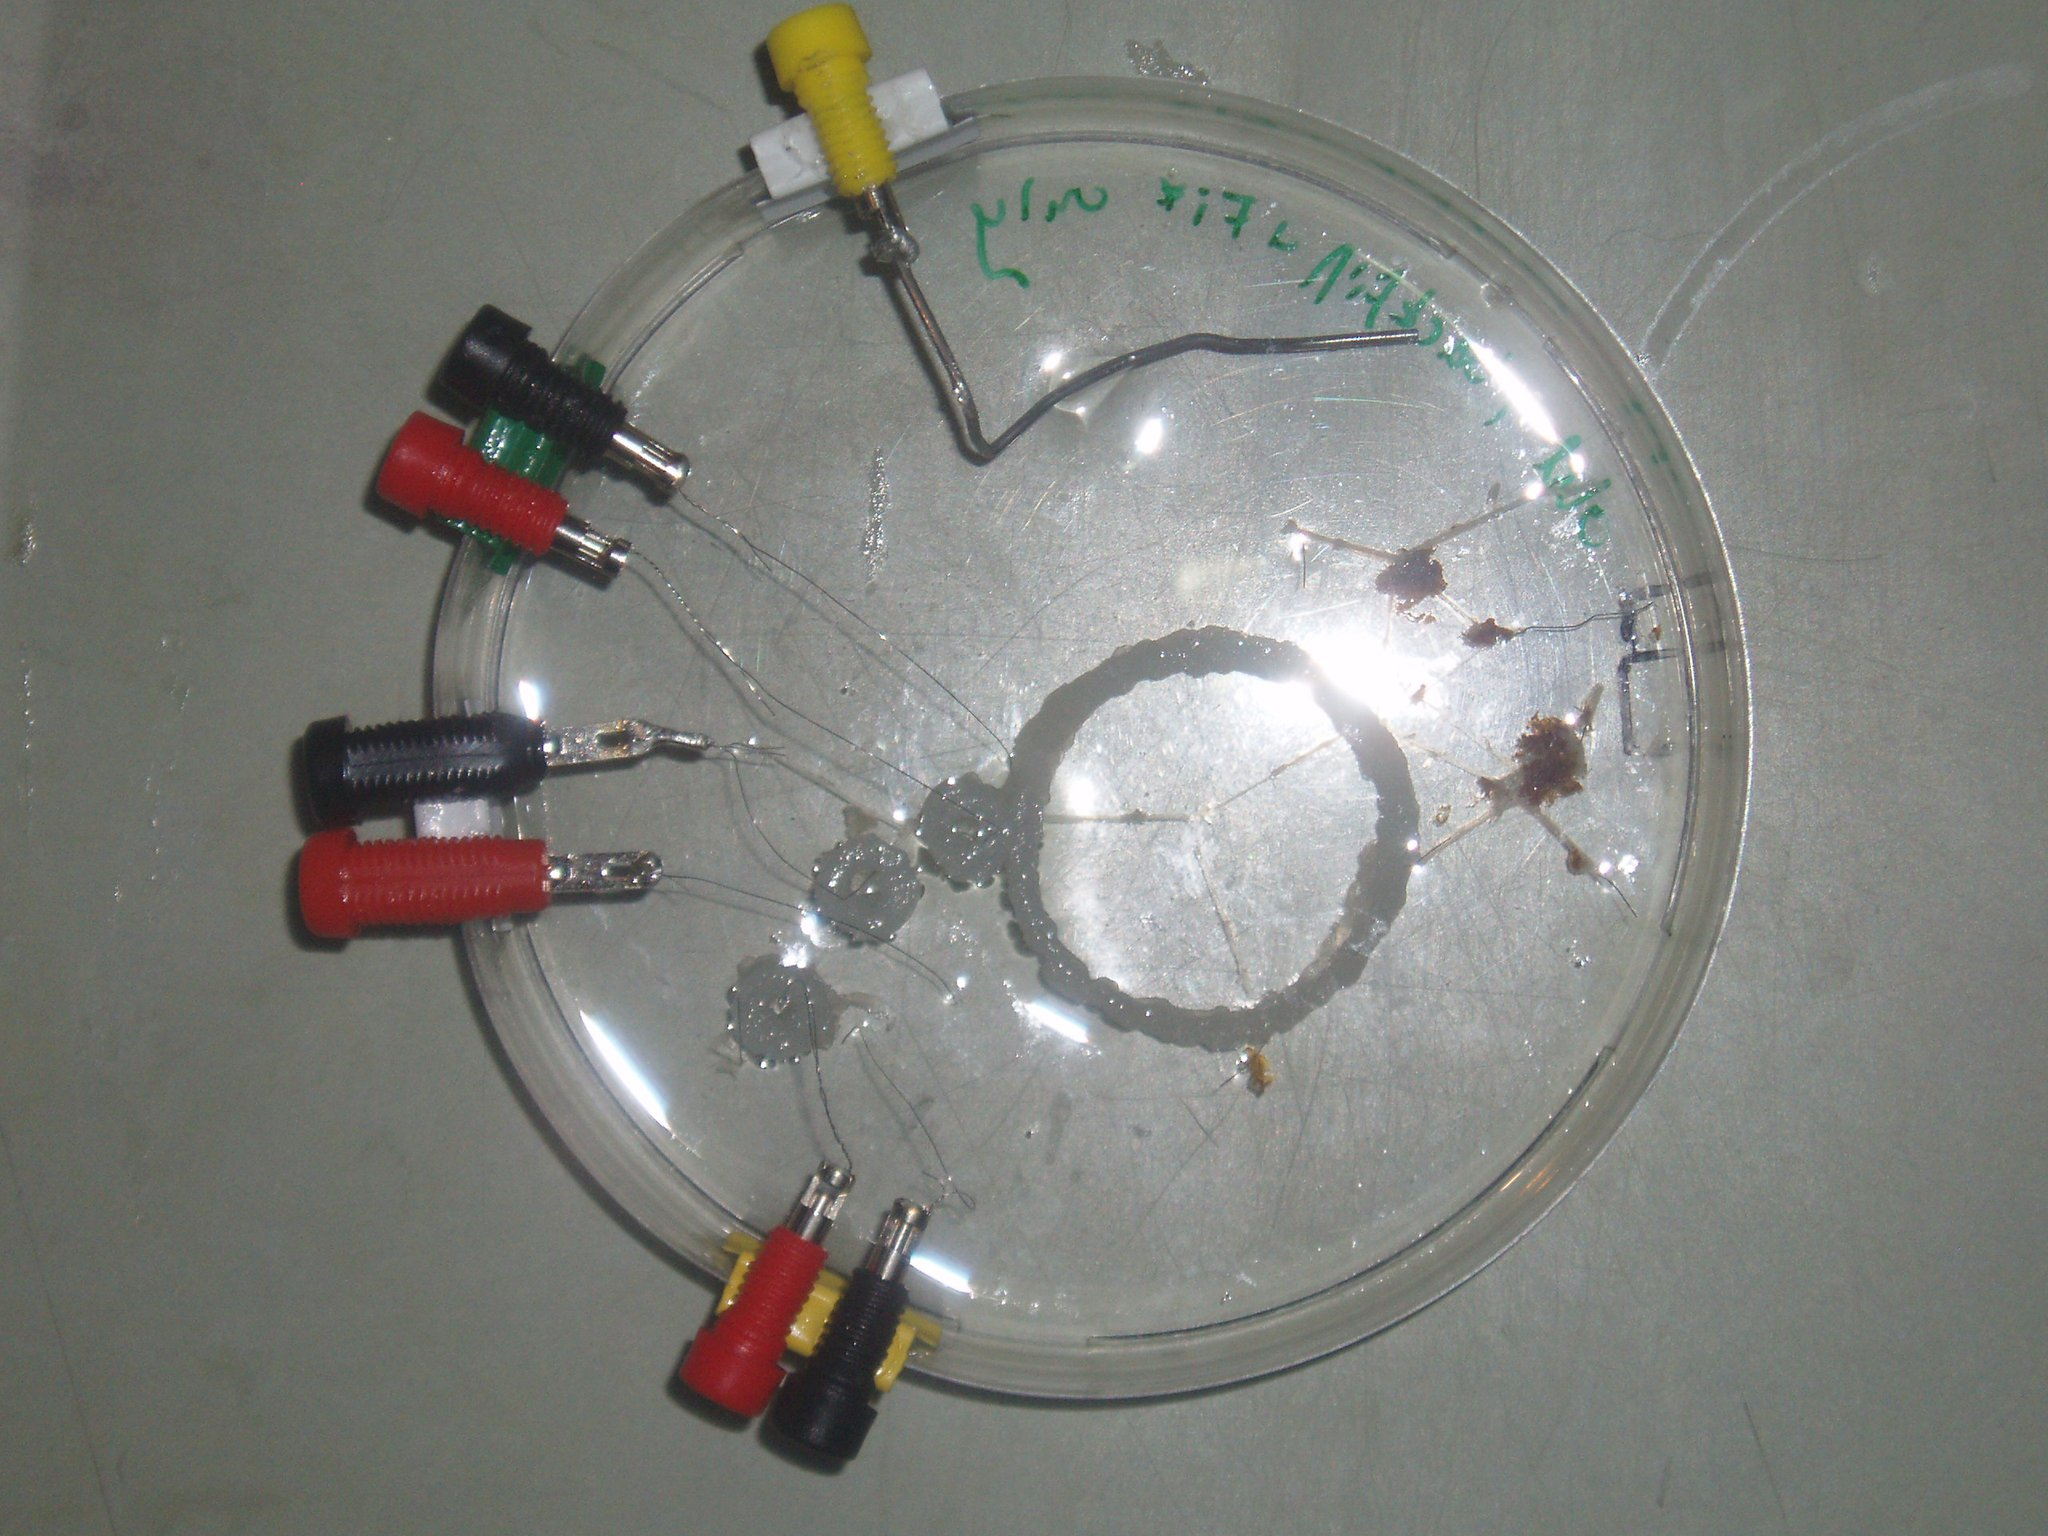
\includegraphics[width=\columnwidth]{graphics/dissection.jpg}
		\caption[The dissected \ac{STNS}]{\textbf{The dissected \ac{STNS}} with 3 small wells over the \ac{dvn} and \ac{lvn} and a large well over the \ac{STG} for the application of dopamine or voltage sensitive dyes.}
		\label{fig:prep}
\end{figure}

\section{Voltage Sensitive Dyes}
\label{sec:vsd}
The planar arrangement of the cell bodies of the \ac{STG} makes this neural system particularly well suited for the recording of multiple neurons using \ac{VSD} imaging. Following the preparation of the crab as described in section \ref{sec:dissection}, neurons are identified using intracellular recording and the analysis of their activity pattern relative to the pyloric rhythm to which these neurons contribute.

Voltage sensitive dyes can be applied intra-cellularly \cite{Stein2011} or extracellularly as a bath application \cite{Staedele2012}. The advantage of bath application is that the dye can be applied to several cells, e.g. the whole \ac{STG} allowing the activity of the whole ganglion to be recorded. The disadvantage of the bath application is that it is significantly more noisy than intra-cellular electrophysiological recordings or intra-cellular dye application recordings. Intra-cellular application of dyes, however, is very time consuming and as such limits the number of neurons that can be filled with the dye before recording can start. The cells required for a specific experiment has to be located first using intra-cellular electrophysiological methods and then filled with dye. Filling takes at least 30 minutes per cell. 

Di-4 ANEPPS\footnote{http://www.lifetechnologies.com/order/catalog/product/P3000MP} was used for bath application of the \ac{STG} in this research. A stock solution is made by dissolving 5mg of Di-4 ANEPPS  in a solution of Pluronic F-127 and 20\% DMSO (dimethylsulfoxide). This stock solution is kept in a fridge at 3 to 5 degrees Celsius. Prior to the bath application, 20 $\mu l$ of stock solution is mixed with 1ml crab saline to give a 10.4024 millimolar solution. A well is made around the desheated \ac{STG} (see Fig. \ref{fig:prep}). The dye is applied to the well and left in the fridge for 20 minutes. The preparation is covered with a blacked out box to prevent exposure to light. After 20 minutes the preparation is removed and placed under the microscope for exposure to a green excitation light at about 450$nm$ while fluorescence emission activity is detected at $>$570$nm$ and captured by a high speed camera such as the MiCAM02 system\footnote{https://tools.lifetechnologies.com/content/sfs/manuals/mp01199.pdf}. 

For imaging using intracellular filling of neurons with voltage sensitive dye, di-8-ANEPPQ dye is used. A stock solution is made by mixing 5 mg dye with 1 ml 20\% F-127 pluronic acid DMSO solution. The dye is applied using intracellular iontophoretic injection with sharp microelectrodes. The tip of a microelectrode with a filament is filled with dye and then back filled with with 3 M KCl. Pulses of 10 nA positive current with a duration of 1.5 s and an interpulse duration of 1.5 s is then used to drive the dye molecules into the cell. To completely load the dye takes 20 to 30 minutes per neuron. The filling procedure is described in detail in \cite{Stein2011}.

Imaging is accompanied by an extracellular recording over the \ac{lvn} or \ac{dvn} which is also used to monitor the state of the preparation. Such a recording provides the well recognised pyloric rhythm (see figure \ref{fig:pyloric_rhythm}) and any change in this rhythm would indicate a state change of the preparation, usually temperature, perfusion or toxicity of the \ac{VSD}. To avoid damage to the preparation the temperature and perfusion needs to be kept constant. A major drawback of \acp{VSD} is photo-toxicity which limits the life of the preparation used \cite{Scanziani2009}. Therefore, imaging bursts are kept short. 

\begin{figure}[H]
	\centering
	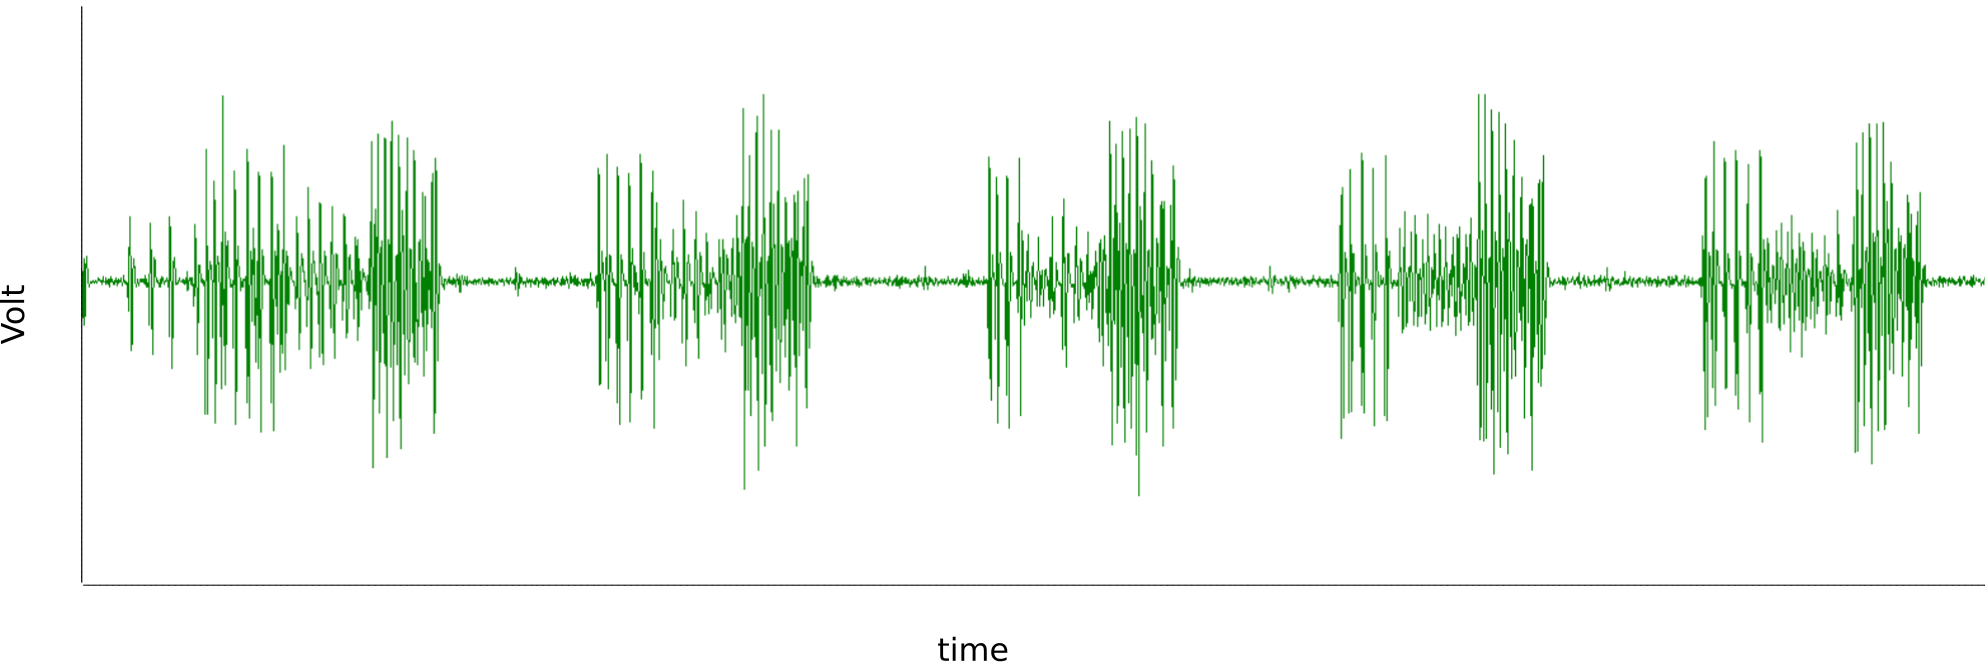
\includegraphics[width=\columnwidth]{graphics/pyloric_rhythm.png}
	\caption[Pyloric rhythm as measured over the \ac{lvn}]{\textbf{Pyloric rhythm as measured over the \ac{lvn}}} 
	\label{fig:pyloric_rhythm}
\end{figure}

Imaging is started by capturing a high resolution image of 376 by 252 pixels. The high resolution image is used for identifying the neuron outlines which is very difficult to do on a low resolution image. After the high resolution image, neural activity is captured with low resolutions images of 40 by 28 pixels. Three short bursts of 21840 frames are captured which have a duration of about 32 seconds each.

\begin{figure}[H]
	\centering
		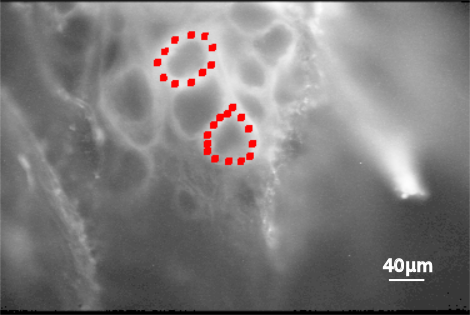
\includegraphics[width=\columnwidth]{graphics/vsd_hires.png}
		\caption[High resolution \ac{VSD} image.]{\textbf{High resolution \ac{VSD} image.} The high resolution image is used for identifying the outlines of the neurons. For illustrative purposes, two neurons have been outlined with red dots. The red outline is overlaid onto the low resolution image below (\ref{fig:vsd_lowres})}
		\label{fig:vsd_hires}
\end{figure}
\begin{figure}[H]
	\centering
		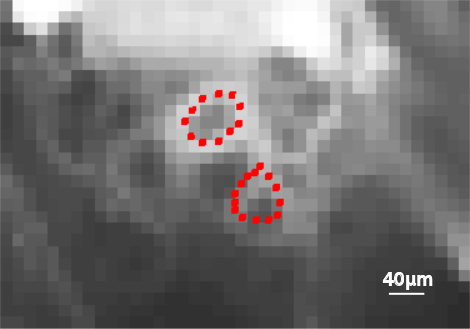
\includegraphics[width=\columnwidth]{graphics/vsd_lowres.png}
		\caption[Low resolution \ac{VSD} images.]{\textbf{Low resolution \ac{VSD} images.} Low resolution images are used for capturing neural activity. These images are difficult to use for identifying the positions of the neurons within the image. This image has been enlarged for illustrative purposes. The mask created on the high res image can be overlaid on the low resolution image. For data analysis the mask from the high resolution image is scaled down to fit the low resolution image.}
		\label{fig:vsd_lowres}
\end{figure}

The \ac{STG} is imaged using a SciMedia MiCAM02 imaging system (SciMedia, Tokyo, Japan). Data is collected with 1.5ms temporal resolution (i.e. 666 images per second) and each neuron is covered by at least 20 pixels in the imaging data.

In this chapter the electrophysiology and \ac{VSD} techniques used for accumulating data were discussed. These data were used to verify the validity of the model which is discussed in chapter \ref{chap:analysis}. It was, however, also necessary to develop methods for the analysis of \ac{VSD} data as no suitable numerical methods exist for this purpose. The next chapter discusses the methods developed that were used to quantify neural activity recorded with \ac{VSD}, such that the de-synchronisation could determined.%Methods and Materials
	\chapter{Methods for the analysis of Dynamics of Temporal Relationships of Neural Activities Using Noisy Optical Imaging Data}	
\label{chap:analysis}
\section{Methods}


The first step in scientific investigation is usually the collection of data. Once the data is collected it needs to be analysed and processed to allow for interpretation within the context of what is already known. \ac{VSD} data allow us to record intracellularly from significantly more neurons at the same time than what electrophysiological techniques allow us to record but at the same time the data is more noisy and thus need different methods for analysis. In the next sections we discuss the methods we have devised for the analysis of injected and bath-applied \ac{VSD} to the \ac{STG} of the brown crab (\species{Cancer pagurus})

The dynamics of the temporal relationship of the activities of neurons forming neural circuits is critically important for the flexible and adaptive delivery of the functionality of the circuits \cite{Harris-Warrick1992,Galan2004,Hill2012,Bruno2015}. For example, switching between synchronised and de-synchronised patterns of activity of neurons forming functional circuits in the hippocampus plays a fundamental role in memory formation, maintenance and recall in vertebrate brains \cite{Axmacher2006,Robbe2006}. In the case of epilepsy a switch to excessive synchronisation of neural activities breaks down the functionality of many neural circuits and the neural systems formed by them \cite{FeldtMuldoon2013, Engel2013}. Recently it has been shown that the fine timing of inputs to different parts of the dendritic tree of neurons in the visual cortex of mammals determines the actual receptive field of the neuron \cite{Chen2013}. In general, both relatively simple and complex changes in the temporal relationship of neural activities can play a critical role in the delivery of the functionality of neural circuits.

While multi-electrode arrays allow recording of many individual neurons in artificially created cell culture \cite{Potter2001, Spira2013}, the activity of neurons in such context is not truly comparable to the activity of neurons in real physiological conditions. In other settings, when multi-electrode array or multiple multi-electrodes (e.g. tetrodes) are used to record many neurons from brains or brain slices in physiological conditions, the connectivity between the recorded neurons is usually not known \cite{Guitchounts2013, Scholvin2015, Santos2012}. the impact of this is that a large part of the work on neuron resolution dynamics of neural circuits remained mostly theoretical \cite{Schneidman2006, Shlens2006, Paninski2010}.

Currently used techniques of optical recording of neural activity using voltage-sensitive dyes and calcium dyes allow high spatio-temporal resolution recording of the activity of many neurons, making possible the study of the dynamics of temporal relationships of neural activities in biological neural circuits \cite{Canepari2010}. While many applications of these techniques are used to record many neurons that are not necessarily directly coupled synaptically \cite{Mukamel2009, Rothschild2010}, it has been shown that these methods can also be applied successfully to a range of biological neural systems to record the activity of many synaptically coupled neurons simultaneously. These techniques have been applied to analyse the functionality of neurons in leech ganglia \cite{Briggman2010}, to study the dynamical assignment of functional roles to neurons in snail ganglia \cite{Hill2012, Bruno2015}, to record almost simultaneously the activity of all neurons in the brain of the zebra fish embryo \cite{Ahrens2012}, to analyse the activity of neurons in intestinal neural ganglia in guinea pigs \cite{Obaid1999}, and to study the activity of synaptically coupled neurons in the stomatogastric ganglion of crabs \cite{Stein2011, Staedele2012}.  However, it should be noted that usually the recorded data is quite noisy, potentially making its analysis difficult.
	
	
\section{De-trending and Event Triggered Averaging}
\label{sec:detrend}
The different types of neurons of the \ac{STG} can be identified by intracellular recordings. Each type of neuron has a distinct shaped voltage waveform that it produces. To confirm the identification of the neuron the voltage waveform is also correlated to extracellularly recorded spikes from the motor nerves. When using \ac{VSD}, the identification of the neurons are more difficult due to baseline drift and noise obscuring the wave forms.  A \ac{VSD} recording is seldom clear enough to discern any spikes. It is, however, possible to obtain a voltage wave form good enough for identifying the recognisable wave features of a specific neuron by first de-trending and then averaging the captured data.

\begin{figure}[H]
	\centering
		\includegraphics[height=17cm]{graphics/ident_neurons.png}
		\caption[Identifying pyloric \ac{CPG} neurons.]{\textbf{Identifying pyloric \ac{CPG} neurons.} Neurons of the pyloric \ac{CPG} can be identified by features of the voltage waveform as well as correlating the waveform to extracellularly recorded spikes from motor nerves. The voltage waveforms of the \acp{PY}, \acp{PD}, \ac{LP} and \ac{VD} are shown here. The horizontal shaded line correlates the waveform with extracellular recordings that were made over the \ac{lvn} and \ac{mvn}. The red arrow points to features typical of the specific neurons \footnote{From the Nadim, Golowasch, Bucher STG website at \url{http://stg.rutgers.edu/resources/Cancer_Guide.pdf}.}. Recording such as these are made using electrophysiological techniques.}
		\label{fig:ident_neurons}
\end{figure}

A trend in a time series is gradual change in some property of the the series of the time interval under investigation. During recordings with \acp{VSD} a decaying trend can often be observed, which can be attributed to dye bleaching \cite{Briggman2010}. 

De-trending on data was done with an R implementation of the following equation which uses a linear approximation of $x_{t}$ as a function of time:

\begin{equation}
\label{eq:detrend}
(m_{i}^{*},b_{i}^{*}) = \frac{argmin}{m,b}\sum_{t=i}^{i+w}\|x_{t}-m\cdot(t-i)-b\|^{2} 
\end{equation}

\begin{equation}
\begin{array}{c c }
y_{i}=x_{i}-m_{i}^{*}\cdot i - b_{i}^{*} \nonumber
\\
i=1,\ldots,z \nonumber
\end{array}
\end{equation}

where:

$m$ is the slope of the linear approximation.

$b$ is the bias or y-intersection of the approximation.

$w$ is the chosen window size.

An appropriate window size needs to be chosen for de-trending. The result of applying equation \ref{eq:detrend} to a recording can be seen in figure \ref{fig:baseline_drift}.

\begin{figure}[H]
	\begin{center}
		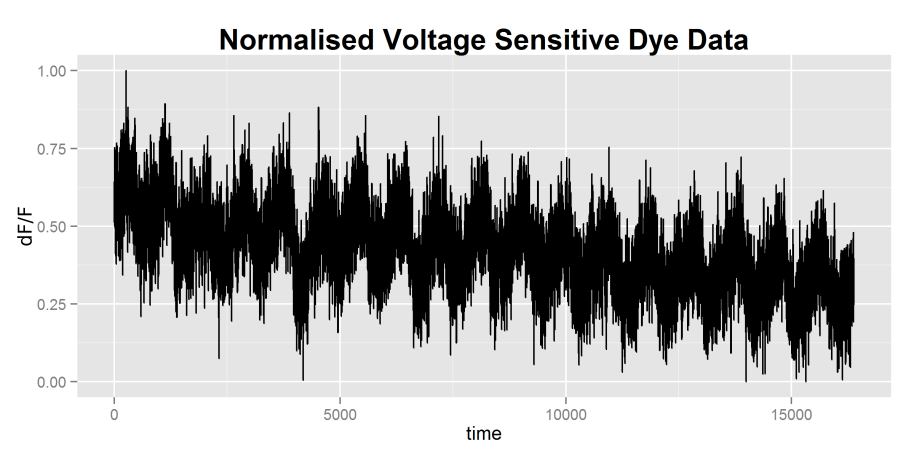
\includegraphics[width=\textwidth]{graphics/data_trending.png}
		\label{fig:trending}
		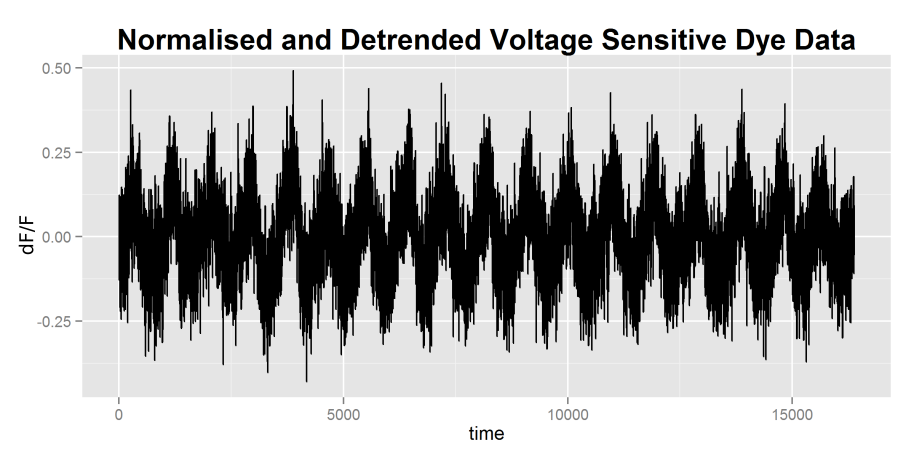
\includegraphics[width=\textwidth]{graphics/data_detrend.png}
		\label{fig:detrending}
		\caption[Neural activity before and after detrending.]{\textbf{Neural activity before and after detrending.} Top: Normalised raw data series from voltage dye imaging without detrending. Bottom: Data series after detrending.}
		\label{fig:baseline_drift}
	\end{center}
\end{figure}

After de-trending averaging over phases of the rhythm has to be done. Averaging requires an extracellular recording that can be used to determine the beginning of each phase. The identification of phases has to be done manually by looking at the trace and noting the time stamp of the first spike in a phase. Spike2 software was used for doing the identification as it allows one to zoom in on a trace to find an accurate time stamp. Figure \ref{fig:data_phases} shows an extracellular recording of the pyloric rhythm made over the \ac{dvn}. The vertical red lines indicate the beginning of each phase. The time values of the occurrence of the first spike of each phase is noted.

\begin{figure}[H]
	\begin{center}
		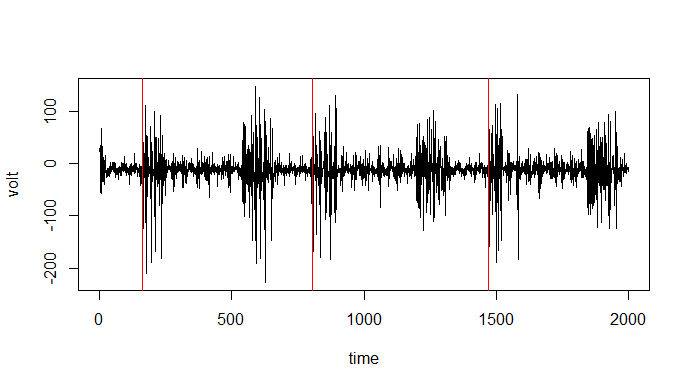
\includegraphics[width=0.8\textwidth]{graphics/data_phases.png}
		\caption[Extracellular recording of the pyloric rhythm.]{\textbf{Extracellular recording of the pyloric rhythm made over the \ac{dvn}}. The vertical red lines indicate the beginning of each phase. The time values of the occurrence of the first spike of each phase is used for doing averaging of the phases. Shown here are only three phases but as many phases as possible should be identified for more accurate averaging.}
		\label{fig:data_phases}
	\end{center}
\end{figure}

At this point it is necessary to decide over how many phases the averaging needs to be done. Let us call the number of phases $p$. Typically, for this research, the decision was made to average over three phases as averaging artefacts on the first and last phase often made them unsuitable for use. Three phases proved to be adequate to identify a neuron against the extracellular recording and also gives enough information for further analysis as described in the following text. Starting at the beginning of each identified phase, the data are placed in arrays, where each array contains $p$ phases. The phases are never exactly the same length, making it necessary to find the length, in time units, of the shortest array of phases. Let us call the length of the shortest phase $l$ and $a$ the number of arrays that can be extracted from the data. If $n$ is the number of phases identified then the number of arrays will be:

\begin{equation}
a=n-p+1
\end{equation}

at each time unit in each array, sum the value of the time points and divide by the number of arrays (see figure \ref{fig:averaging}) to give an average for that time point. Averaging is done up to the length of the shortest array ($l$).  The fact that the arrays are not the same length accounts for the artefacts that are sometimes observed in the last phase which can make it unusable. 

\begin{figure}[H]
	\begin{center}
		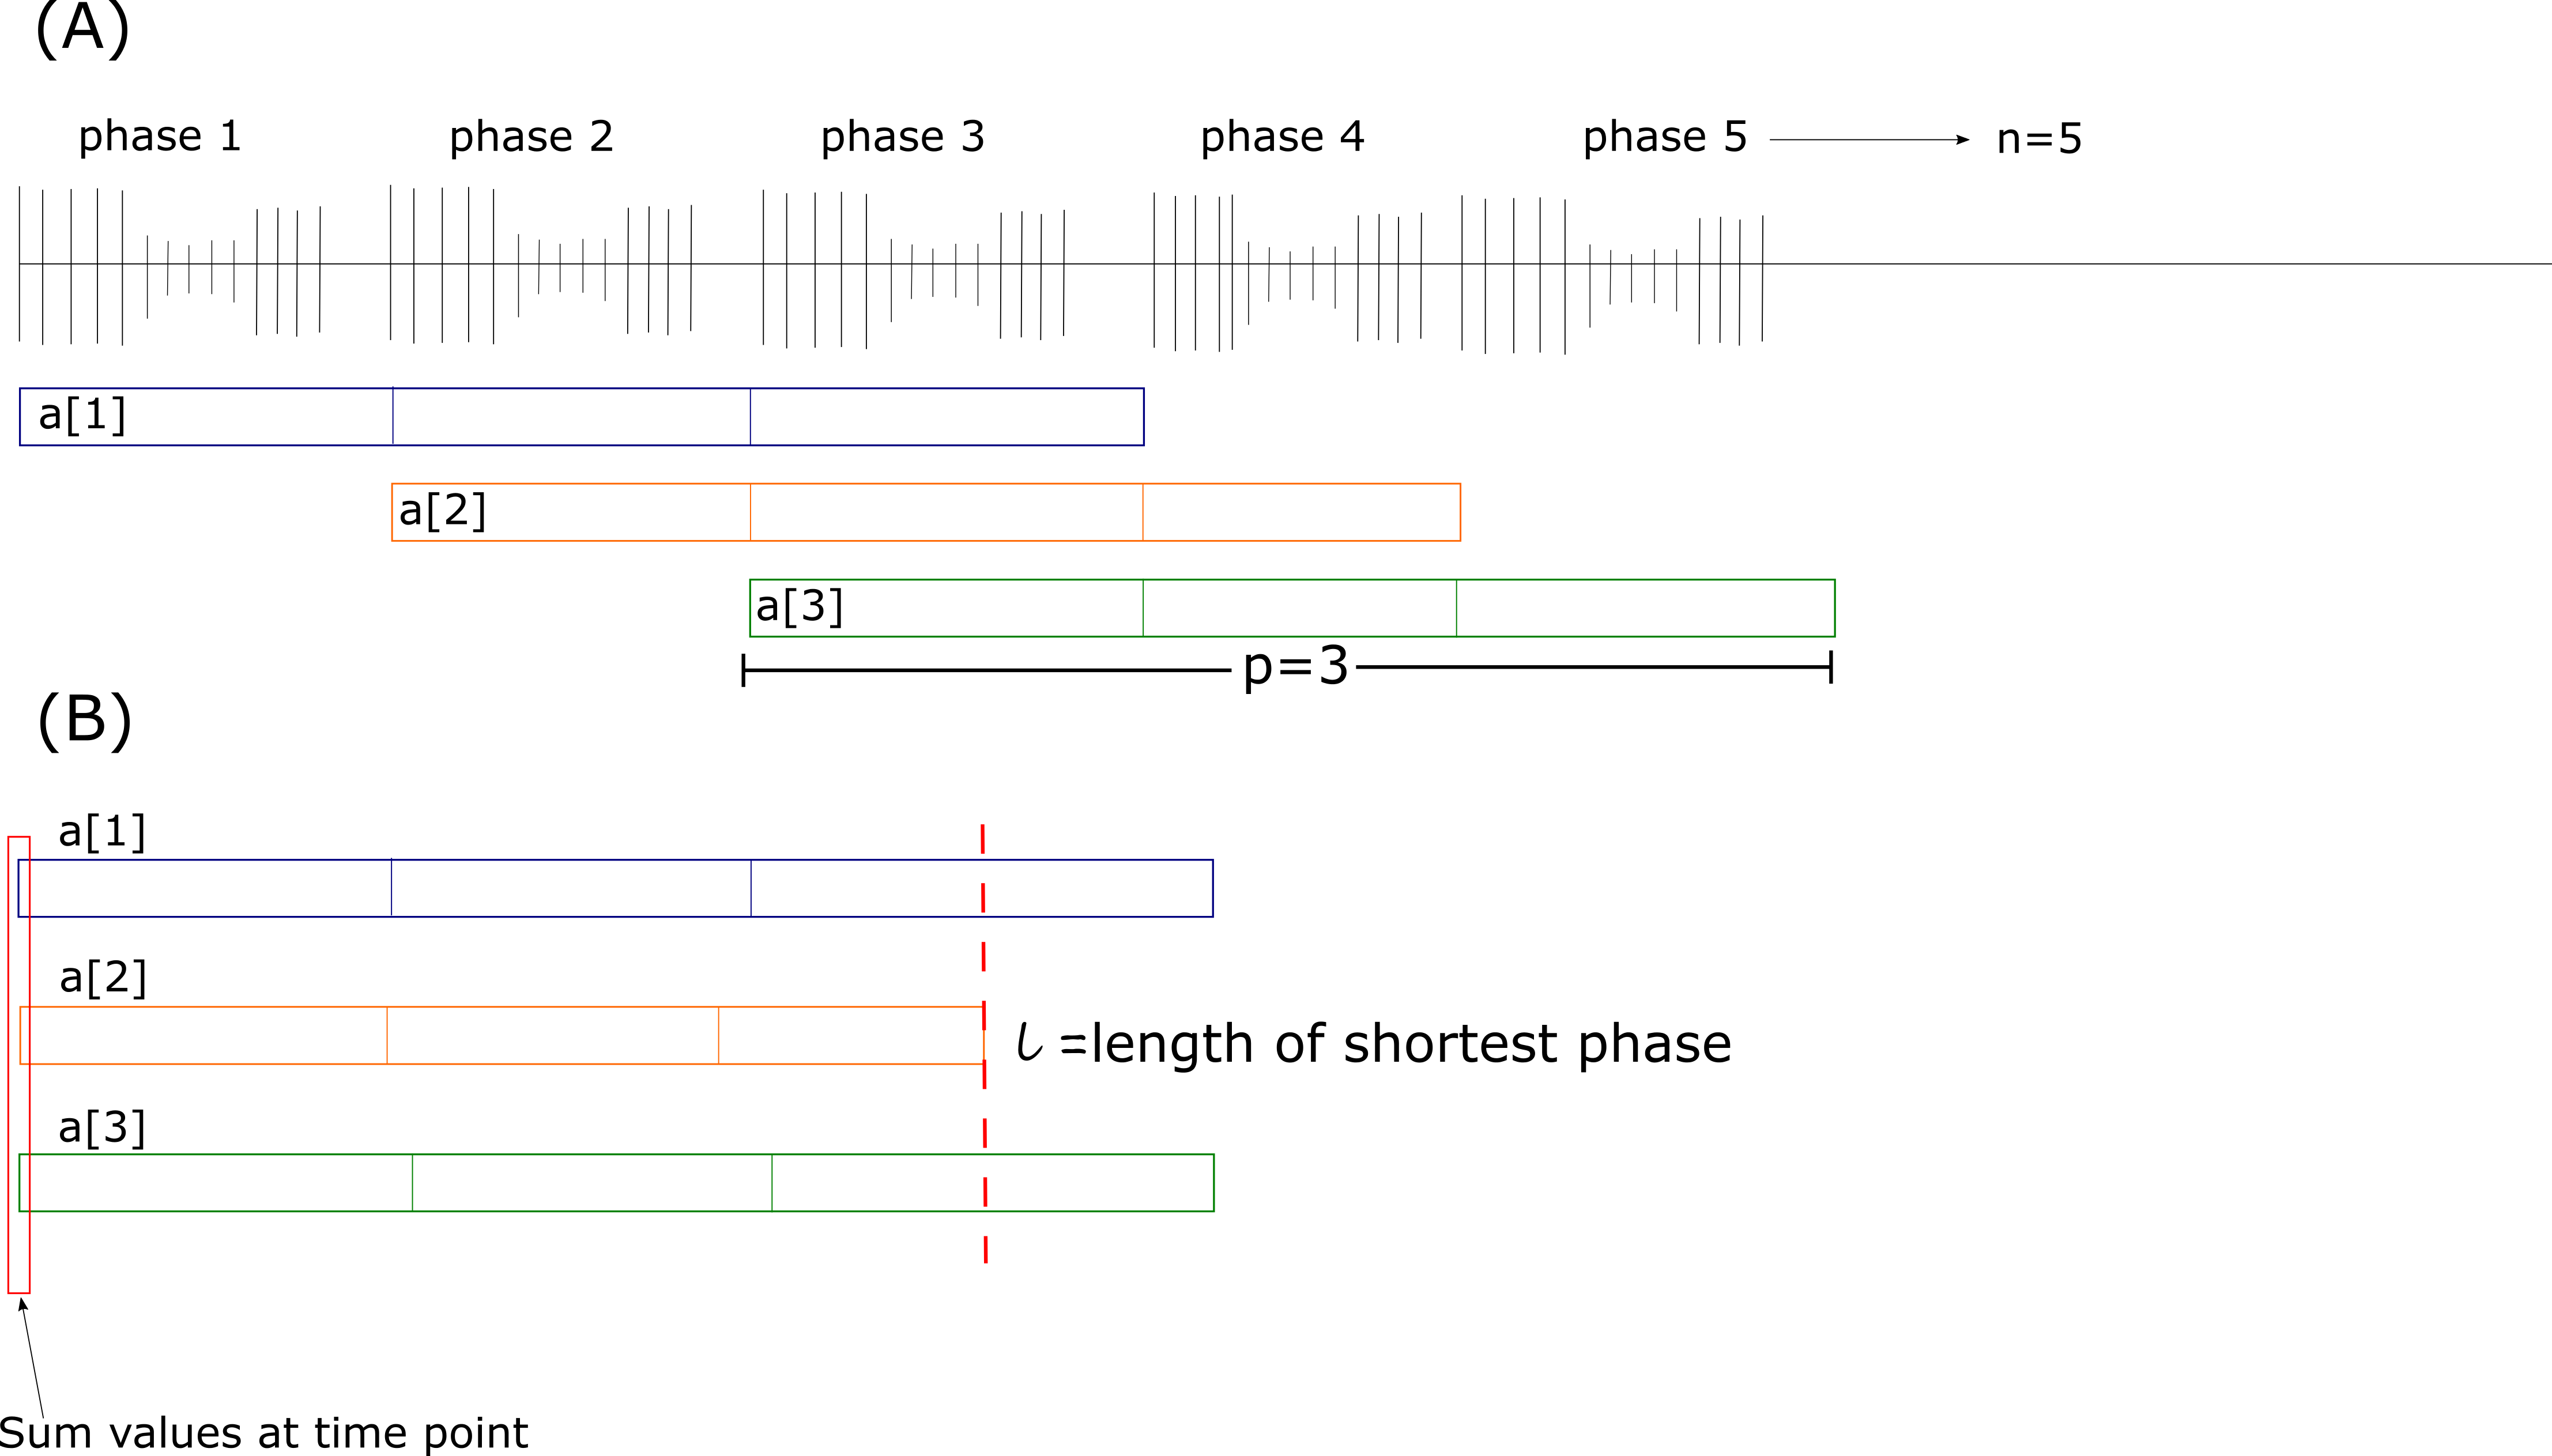
\includegraphics[width=\columnwidth]{graphics/averaging.png}
		\caption[Event-triggered averaging.]{\textbf{Event-triggered averaging.} (A) illustrates the identification of phases in a time series. Five phases are identified (n=5) in this example. The data are placed in arrays where each array contains $p$ phases (p=3). (B) illustrates the summing of each time point over all the arrays. The sum is then divided by the number of arrays to get the average for that time point. This averaging is done for all time points up to the length of the shortest array ($l$), indicated by the dotted red line. }
		\label{fig:averaging}
	\end{center}
\end{figure}

Figure \ref{fig:averaged} shows an averaged time series. This averaging methods works well for both intra- and extracellularly applied \ac{VSD} recordings. 
\begin{figure}[H]
	\begin{center}
		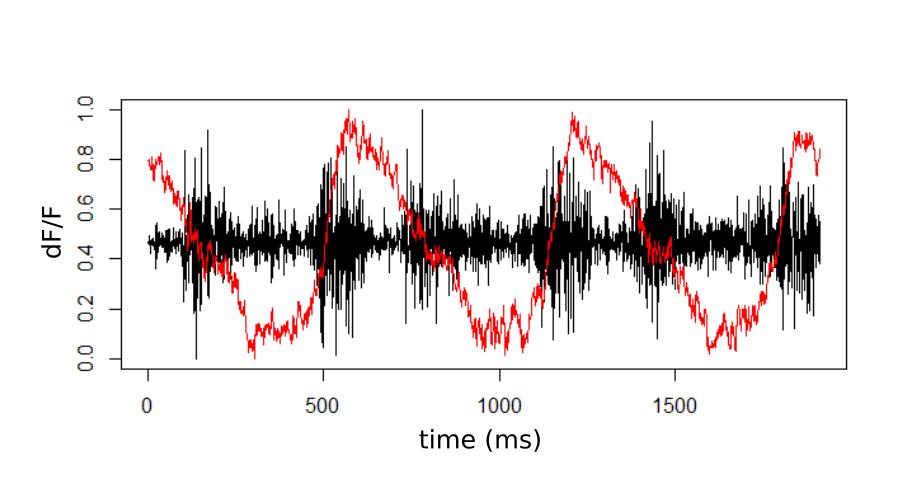
\includegraphics[width=\columnwidth]{graphics/averaged.png}
		\caption[Averaged intra- and extracellular recording.]{\textbf{Averaged intra- and extracellular recording.} The black trace shows an extracellular recording averaged over three phases. The red trace is the averaged data from figure \ref{fig:baseline_drift} overlaid onto the extracellular recording, illustrating the correlation of the voltage sensitive dye recording with the extracellular recording and how the shape of the wave becomes apparent after averaging. To be able to overlay the data as in this figure, it is necessary to normalise both traces. In this case, normalisation was done to values between 0 and 1.}
		\label{fig:averaged}
	\end{center}
\end{figure}

\section{Analysis of Noisy Optical Imaging Data}
\label{sec:analysis_methods}

Using the \ac{VSD} imaging techniques described in section \ref{sec:vsd} the \ac{STG} was first imaged in normal saline. For the purpose of dopamine exposure the \ac{STG} was perfused with saline containing dopamine. First a saline solution containing $10^{-6}M$ concentration dopamine was applied to the \ac{STG} for 20 minutes. This condition is called the ``low dopamine'' condition. After the initial 20 minute exposure to dopamine, perfusion with the dopamine saline solution was maintained while imaging. Next, a saline solution containing $10_{-4}M$ concentration dopamine (i.e. 100 times more dopamine than in the previous experimental condition) was used and the \ac{STG} was exposed to this for 20 minutes. This condition is called the ``high dopamine'' condition. The preparation was imaged again while perfusion with the high dopamine saline solution is maintained.

The activity of neurons participating in biological neural circuits follows various patterns. Some neurons are silent most of the time balancing around their resting potential, on occasion firing a single or a few spikes, for example many cortical neurons in mammals \cite{Brumberg2000}. Other neurons, such as invertebrate neurons that form central pattern generators, periodically generate bursts of activity \cite{Harris-Warrick1992}. One relatively common feature of the various neural activities is that, generally, the spiking of neurons (especially multiple spikes) happens on the top of a depolarization plateau (fig \ref{fig:spikes}). 

\begin{figure}[H]
	\begin{center}
		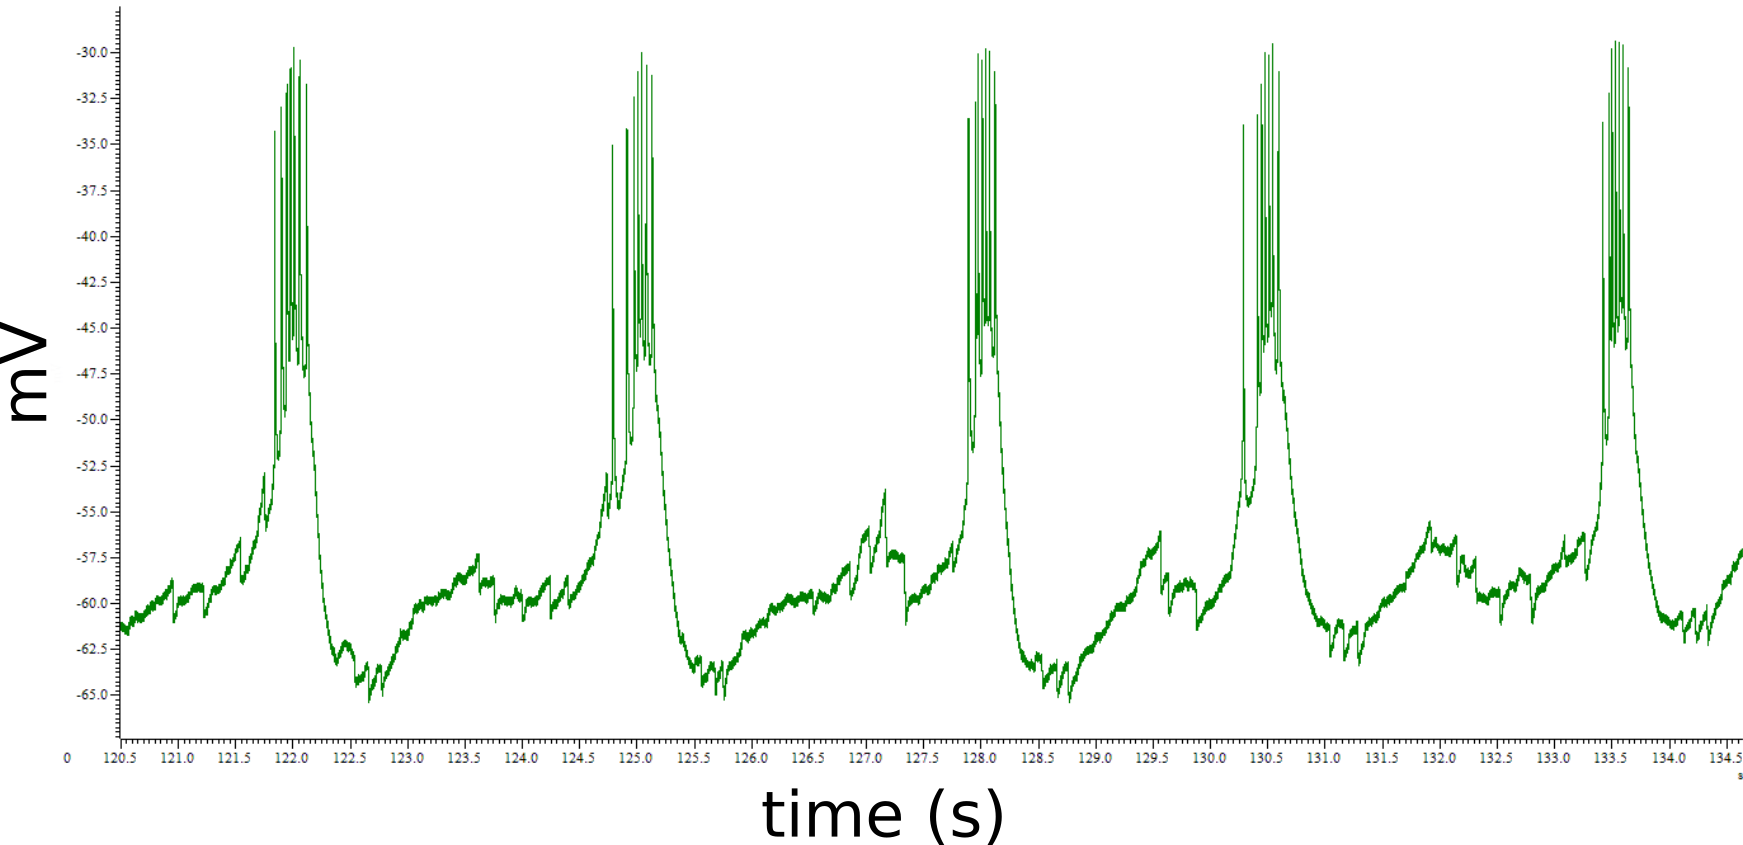
\includegraphics[width=\columnwidth]{graphics/PD_intra.png}
		\caption[Intracellular recording of \ac{STG} neuron.]{\textbf{Intracellular recording of \ac{STG} neuron.} Intracellular recording of a neuron from the crab stomatogastric ganglion. The spiking of neurons (especially multiple spikes) happens on the top of a depolarization plateau.}
		\label{fig:spikes}
	\end{center}
\end{figure}

In some cases the amplitude of membrane potential difference deviations during the spikes is larger (possibly much larger) than the amplitude of depolarization for the plateau \cite{Brumberg2000}. In other cases the depolarization amplitude of the plateau can be of a comparable size or even larger than the amplitude of the of the membrane potential difference changes during spikes \cite{Harris-Warrick1992} (fig \ref{fig:spike_comparison}). 

\begin{figure}[H]
	\begin{center}
		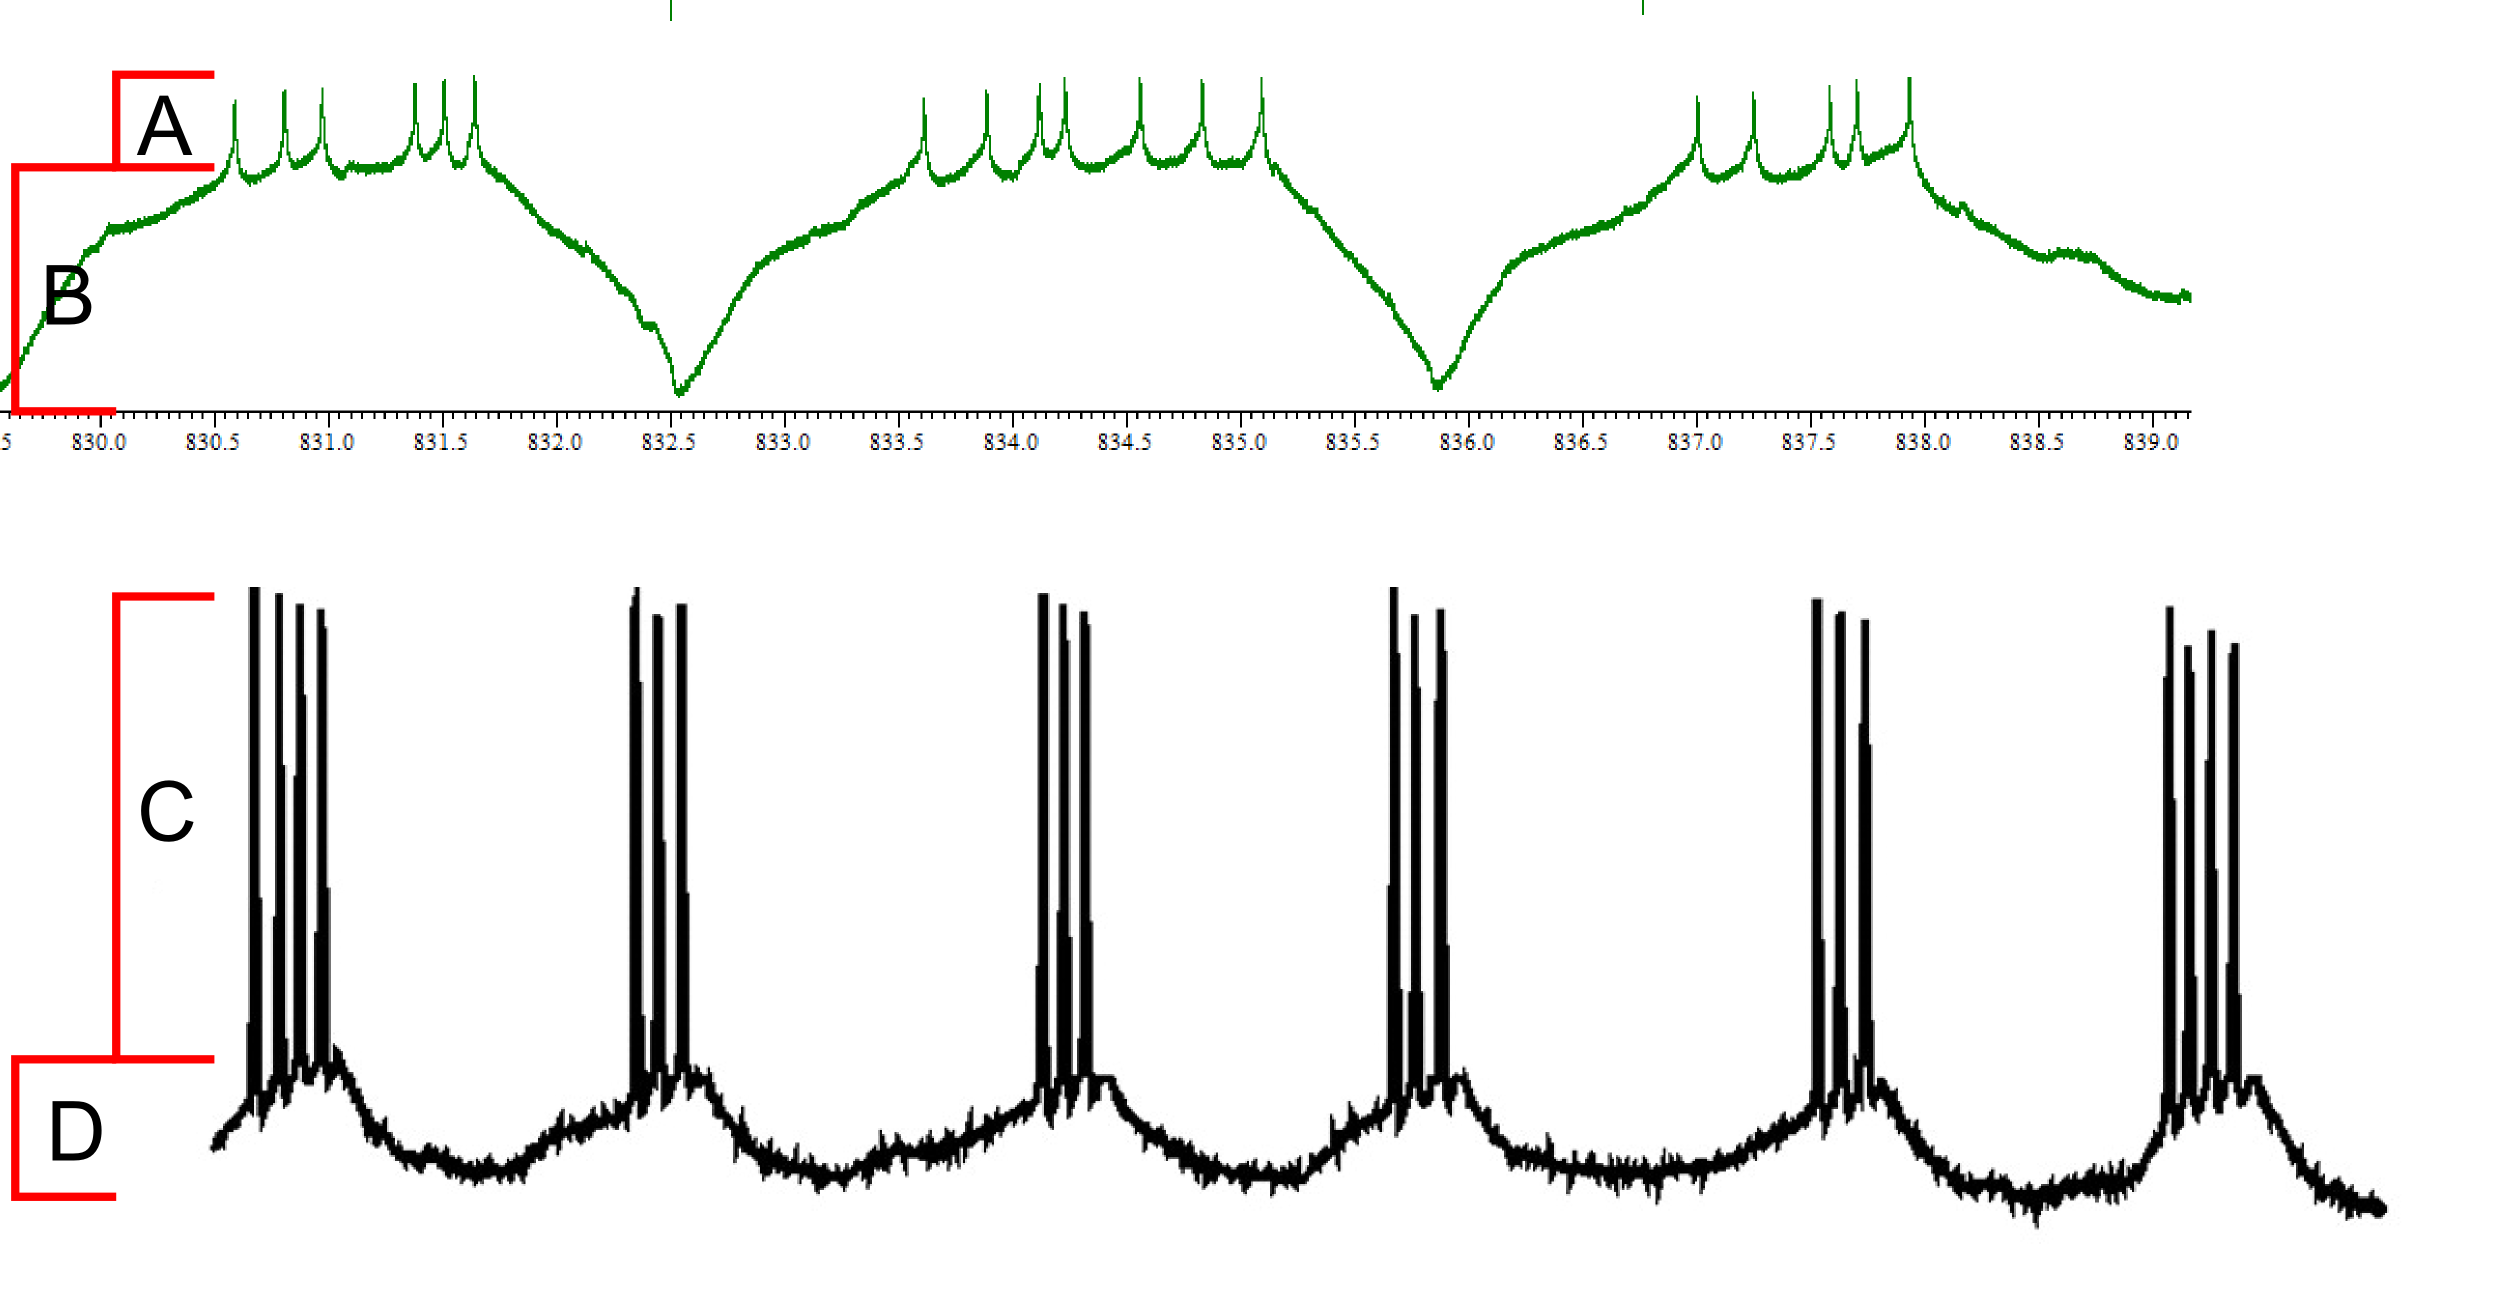
\includegraphics[width=\columnwidth]{graphics/Spikes_comparison.png}
		\caption[Comparison of mammalian and invertebrate neural spikes. ]{\textbf{Comparison of mammalian and invertebrate neural spikes.} The trace at the top is an intracellular recording of a neuron in the crab stomatogastric ganglion. Typical of invertebrate spikes, the amplitude of the spikes (A) is smaller than the depolarisation amplitude of the plateau (B). In the case of mammalian spikes, the amplitude of the spikes (C) are much larger than the amplitude of the plateau (D). (Mammalian spikes from \cite{Wang1999}.)}
		\label{fig:spike_comparison}
	\end{center}
\end{figure}
%\note{\cite{Wang1999,Wang2010,Gray1996}}

In general the change in the relative temporal ordering of the activity of multiple neurons is reflected by changes in the relative timing of individual spikes or bursts of spikes generated by these neurons. Thus, the temporal dynamics of relative activities of neurons is reflected also by the dynamics of the relative timing of activity plateaus of these neurons.

In the case of micro-electrode intra-cellular recording of neurons individual spikes, even as part of a burst of spikes, can easily be distinguished. In the case of optical imaging recording of neural activities, this is often not the case due to inherent noise of imaging. This means that relying on the determination of spike and burst times of individual neurons is relatively difficult and the use of these neural activity markers is relatively unreliable for the estimation of the dynamics of the temporal relationships of the neural activities.

In this section, the use of the timing of the activity plateaus of neurons for the estimation of the dynamics of the temporal relationships of their activities is proposed. The proposed heuristic analysis works off-line, following the recording of the activity of the neurons. In order to use activity plateaus for this purpose a set of salient features of these that can be determined robustly using the noisy optical imaging data needs to be defined. Given that, in general, the activity plateaus are preceded by a ramp-up phase and are followed by a ramp-down phase of the membrane potential in the soma of the neuron, the salient features of neural activity profile that are chosen are indicators of the timing of the ramp-up, ramp-down and the beginning and ending of the plateau itself (fig \ref{fig:activity_profile}).

\begin{figure}[H]
	\begin{center}
		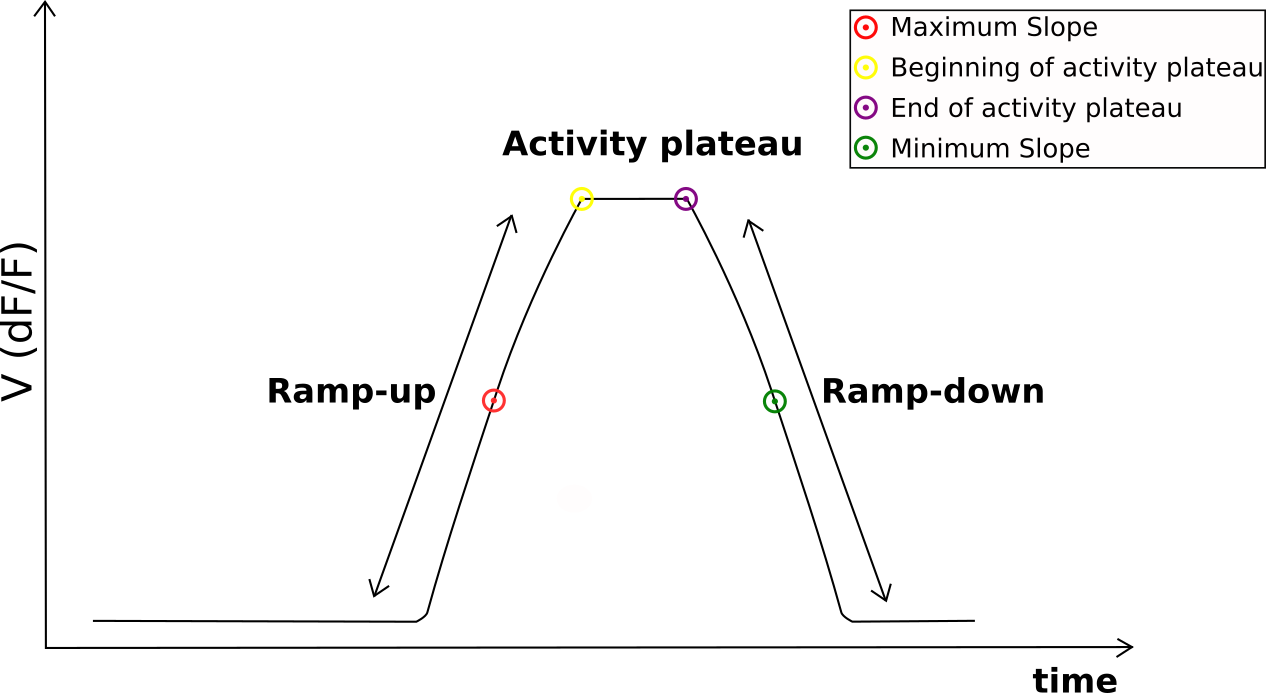
\includegraphics[width=\columnwidth]{graphics/activity_profile.png}
		\caption[Typical activity profile of a neuron.]{\textbf{Typical activity profile of a neuron.} The spiking happens during the activity plateau, which is preceded by the ramp-up phase and followed by the ramp-down phase. The vertical axis shows the membrane potential of the neuron.}
		\label{fig:activity_profile}
	\end{center}
\end{figure}

To find the timing of the ramp-up phase, the time point for which the upward slope of the neural activity profile is maximal is numerically determined. An appropriate time interval that lasts for around the usual duration of the measured ramp-up phases has to be chosen. This point is expected to be around the mid-point of the ramp-up phase. To find the \textbf{\textit{maximum upward slope point}} (or maximum slope point, given that the upward slope is a positive slope), the slope of the best linear approximation of the data points representing the neuron's activity profile for an appropriately chosen time window centred on the time of the given time step is calculated for each step. Assuming that $x_{t}$ are the measured values of the neural activity at recording time step $t$, it means that time intervals of $2\tau+1$ measurement time units is considered and the \textbf{\textit{local slope approximation}} $m_{t}$ is calculated such that:

\begin{equation}
\label{eq:local_slope}
(m_{t},b_{t})=\frac{argmin}{m,b}\sum^{t+\tau}_{u=t-\tau}(x_{t}-m\cdot(u-t+\tau)-b)^2
\end{equation}

The maximum slope point for a time interval $[T_{1},T_{2}]$, measured in units of recording time steps, is the point on the activity profile of the neuron corresponding to the time point $t^{*}$ for which 

\begin{equation}
m_{t^{*}}=\max_{t\in[T_{1},T_{2}]}m_{t}
\end{equation}

If the time interval $[T_{1},T_{2}]$ is chosen such that $T_{2}-T_{1}$ is approximately the usual time length of the ramp up phase (measure in units of recording time steps) and $\tau$ is chosen appropriately (e.g. $\tau=(T_{2}-T_{1})/2$ or slightly less), then it can be expected that the above calculation will find the maximum slope point of the neural activity profile corresponding to the time interval $[T_{1},T_{2}]$. If the chosen time interval is such that during this time interval the neuron's activity profile follows a ramp-up phase, the maximum slope point that is found is likely to indicate the midpoint of the ramp-up phase. If the chosen interval is such that the activity profile of the neuron for this interval does not match a ramp-up phase, the maximum slope point that is found will not indicate the mid-point of a ramp-up phase. Such points are called \textbf{\textit{spurious maximum slope points}}.

To distinguish between maximum slope points which indicate valid mid-points of ramp-up phases and those which do not, the value ranges of the calculated maximum slope values for many considered time intervals have to be considered. If the membrane potential variation associated with the ramp-up phase is larger than the membrane potential variation associated with spikes measured in the neuron soma, the slope values for valid maximum slope points will be much larger than the slope values calculated for spurious maximum slope points.

In general, spurious maximum slope points, calculated for periods of relative silence of neural activity, will have small maximum slope values associated with them (possibly very close to zero). If the soma membrane potential variations associated with spikes are larger than the soma membrane potential variation during the ramp-up phase, some spurious maximum slope points may have larger slope values associated with them than the slope values calculated for valid maximum slope points. In such cases it is necessary to rely on setting the appropriate and sufficiently narrow value interval for valid maximum slope values based on the analysis of the experimental data. Figure \ref{fig:slopes} presents synthetic examples of these two cases demonstrating the determination of the maximum slope points.

\begin{figure}[H]
	\begin{center}
		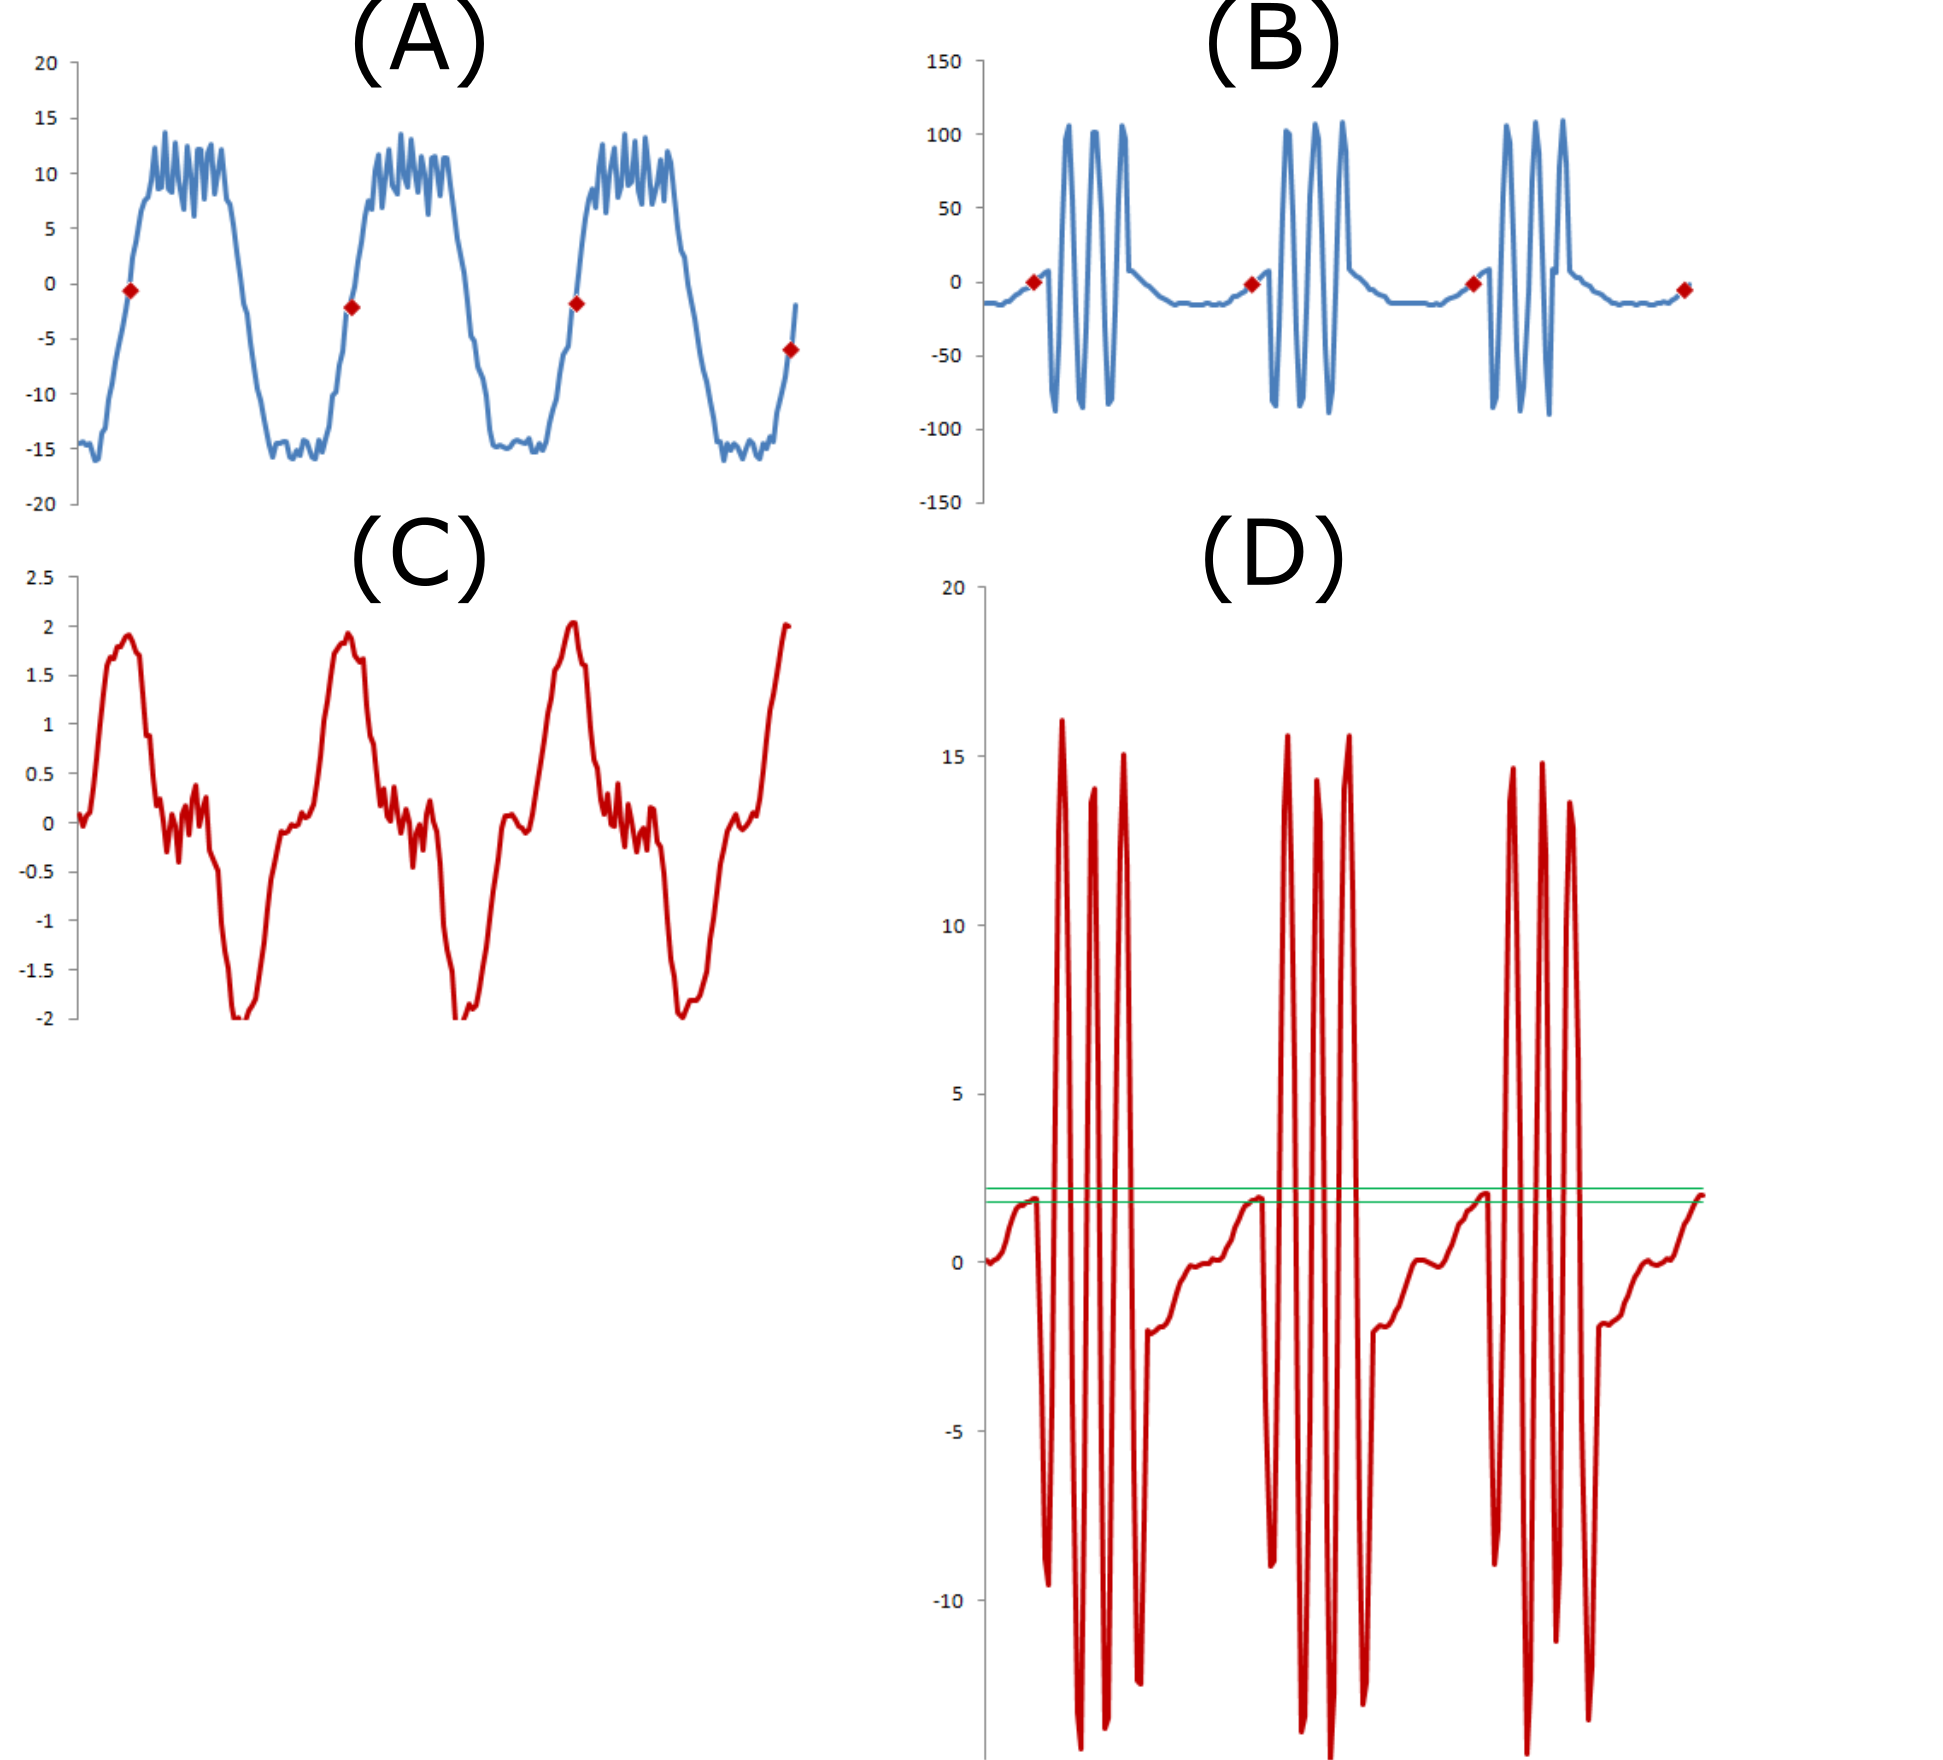
\includegraphics[width=\columnwidth]{graphics/slopes.png}
		\caption[Calculating maximum and local slopes. ]{\textbf{Calculating maximum and local slopes. }(A) Maximum slope points calculated for simulated neural activity having a plateau potential difference that is much larger than the potential difference corresponding to spike activity; (B) The calculated local slope values for the data shown in (A); (C) Maximum slope points calculated for simulated neural activity having a plateau potential difference that is much smaller than the potential difference corresponding to spiking activity; (D) The calculated local slope values for the data shown in (C). The horizontal axis is always time, the vertical axis represents the voltage in (A) and (C) in arbitrary units and the local slope value (B) and (D).}
		\label{fig:slopes}
	\end{center}
\end{figure}

For the timing of the ramp-down phase the time point with the maximal downward slope of the neural activity profile is determined. A method, similar to that used for determining of the maximum slope point is used. In the case of the ramp-down phase the general expectation is that the minimum slope (equivalent to the maximum downward slope) point is around the middle of the ramp-down phase. To find the minimum slope point the calculation for each time stop of the slope of the best linear approximation of the data points representing the neuron's activity profile for an appropriate time window centred on the given time step (Eq.\ref{eq:local_slope}) is used. The minimum slope point for a time interval $[T_{1},T_{2}]$ measured in units of recording time steps is the point on the activity profile of the neuron corresponding to the time point $t^{**}$ for which:

\begin{equation}
\label{eq:min_slope_point}
m_{t^{**}}=\min_{t\in[T_{1},T_{2}]}m_{t}
\end{equation}

As stated previously, for approximately chosen $T_{2}-T_{1}$ and $\tau$ it can be expected that equation \ref{eq:min_slope_point} finds the minimum slope point of the neural activity profile corresponding to the time interval $[T_{1},T_{2}]$. If the chosen interval is such that the activity profile of the neuron for this interval does not match a ramp-down phase, the minimum slope point that is found will not indicate the mid-point of a ramp-down phase, and these are called \textbf{\textit{spurious minimum slope points}} points, similarly to spurious maximum slope points. As in the case of maximum slope points, if the membrane potential change associated with the ramp-down phase is considerably larger than the soma membrane potential change associated with spikes, the valid minimum slope points will be significantly smaller than the spurious minimum slope points, which are expected to have values close to zero. If the membrane potential changes in the soma associated with spikes are larger than the membrane potential change of the ramp-down phase, the determination of the valid minimum slope points relies on the experimental determination of the acceptability range of valid minimum slope values and those minimum slope points are considered valid for which the associated slope value is in this acceptability range.

In the case of neurons with large change of membrane potential difference during ramp-up and ramp-down phases and relatively small changes of the membrane potential difference during the spikes, the calculation of local slope approximation also allows the estimation of the beginning and the end of the activity plateau. The estimation cannot be done reliably for neurons where the membrane potential difference changes in the soma during spiking are much larger than the changes during the ramp-up and ramp-down phases.

To find the estimated points for the beginning and the end of the activity plateau the local forward and backward slopes of the neural activity are considered. The \textbf{\textit{local forward slope}}, at a time point, is the slope of the best linear approximation of the neural activity starting from that time point and for some time period forward. It is expected that the local forward slope gets close to zero around the start of the activity plateau, given that the soma membrane potential difference variations related to spikes are relatively small, and that the local forward slope is considerably positive for time points before the start of the activity plateau. Similarly, the \textbf{\textit{local backward slope}} at a time point is the slope of the best linear approximation of the neural activity over some time period ending at this  time point. In general, it can be expected that the local backward slope is close to zero for time points on the activity plateau and becomes considerably negative as the activity of the neurons goes into the ramp-down phase. So, the end of the activity plateau is indicated by the last time point where the local backward slope is close to zero.The estimated local forward and backward slope, $m_{t}^{f}$ and $m_{t}^{b}$ respectively, are calculated as follows:

\begin{equation}
\label{eq:forward_slope}
(m_{t}^{f},b_{t}^{f}) = \frac{argmin}{m,b}\sum_{u=t}^{t+2\tau}(x_{t}-m\cdot(u-t+\tau)-b)^{2}
\end{equation}

\begin{equation}
\label{eq:backward_slope}
(m_{t}^{b},b_{t}^{b}) = \frac{argmin}{m,b}\sum_{u=t-2\tau}^{t}(x_{t}-m\cdot(u-t+\tau)-b)^{2}
\end{equation}

Next, the points on the activity profile of the neuron for which the calculated local forward and backward slope values are close to zero have to be found. The acceptable range of close to zero values may be determined on a case-by-case basis examining the calculated slope values. In principle the acceptability range may be chosen as $[-\epsilon \cdot m_{max},\epsilon \cdot m_{max}]$, where $m_{max}$ is the maximal absolute value of the calculated slope values associated with maximum and minimum slope points and $\epsilon$ is a small number, for example $\epsilon=0.1$. This range of values is called the \textbf{\textit{zero value range}} and is denoted as $[-z^{*},z^{*}]$. Following the finding of all the points with forward and backward slope values within the zero value range the first of these that follows a maximum slope point and the last that precedes the minimum slope point are determined. These two points will be estimates of the beginning and the end, respectively, of the \textbf{\textit{activity plateau}} of the neuron. In formal terms it is determined as:

\begin{equation}
\label{eq:plateau_begin}
T^{z,f} = \{t|m_{t}^{f} \in [-z^{*},z^{*}]\}
\end{equation}

\begin{equation}
\label{eq:plateau_end}
T^{z,b} = \{t|m_{t}^{b} \in [-z^{*},z^{*}]\}
\end{equation}

then $t_{b}^{0}$ and $t_{e}^{0}$ are determined such that:

\begin{equation}
\label{eq:plateau_time_begin}
t_{b}^{0} > t^{*}, t_{b}^{0} \in T^{z,f},t_{b}^{0} \leq t, \forall t \in T^{z,f},t>t^{*}
\end{equation}

\begin{equation}
\label{eq:plateau_time_end}
t_{e}^{0} > t^{*}, t_{e}^{0} \in T^{z,b},t_{b}^{0} \leq t, \forall t \in T^{z,b},t<t^{*}
\end{equation}

The beginning and end of the activity plateau will be the points corresponding to the time steps $t_{b}^{0}$ and $t_{e}^{0}$ respectively. In general, it should be possible to determine an activity plateau for each consecutive  pair of maximal and  minimal slope points. Figure \ref{fig:min_max_points} exemplifies the determination of maximum and minimum slope points and the beginning and end points of activity plateaus using synthetic data for a neuron with large membrane potential difference changes associated with ramp-up and ramp-down phases and relatively small such changes in the soma associated with spikes.

\begin{figure}[H]
	\begin{center}
		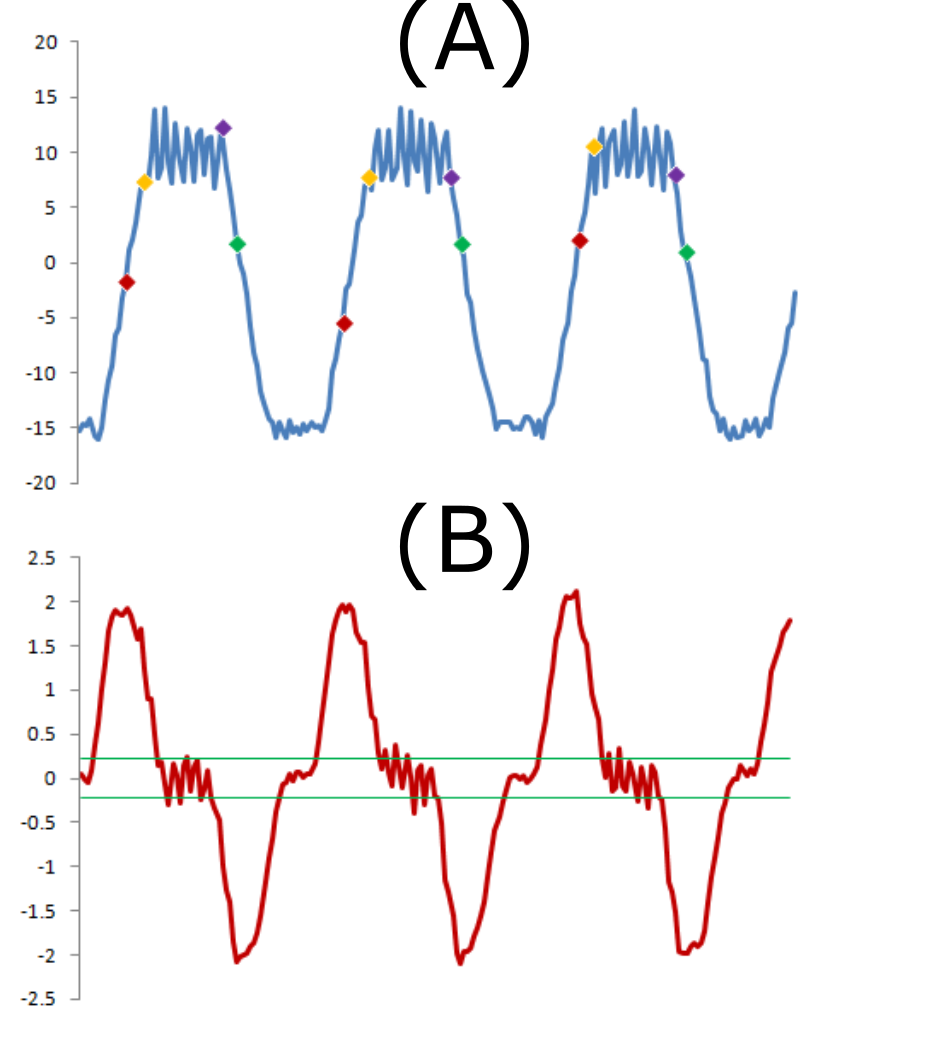
\includegraphics[width=\columnwidth]{graphics/min_max.png}
		\caption[Finding the activity plateau.]{\textbf{Finding the activity plateau.} (A) Simulated activity of a neuron. The \textbf{calculated maximum slopes} are shown as red dots and the \textbf{calculated minimum slopes} are shown as green dots. The beginning  and end points of activity plateaus are shown with yellow and purple dots respectively; (B) The thin green lines indicate the value band that is considered to correspond to the activity plateau following the maximum slope point. The horizontal axis is time in both cases,  while the vertical axis represents voltage in (A) in arbitrary units and the calculated local slope value in (B).}
		\label{fig:min_max_points}
	\end{center}
\end{figure}

Following the determination of maximum and minimum slope points and possibly of the beginning and end points of activity plateaus for multiple neurons recorded simultaneously the timing of these points can be used to analyse the changes in the temporal relationship of the activities of the recorded neurons. Depending on the number of the kinds of salient points determined, multiple estimates about the observable temporal features of the joint activity of the considered neurons can be obtained. For example, the average time difference between maximum slope points of the two rhythmically active neurons indicates the temporal difference between the activation of the neurons, while the average time difference between minimum slope points of the same neurons indicates the temporal difference between the inactivation of these neurons. Phase locking between the neurons is indicated by small standard deviations of  the calculated temporal differences between matching maximum slope or minimum slope points of the neurons and the relaxation of phase locking is implied by an increase of the standard deviation for example following exposure to a neuromodulator.

The robustness of the above proposed calculations can be assessed by considering $x_{t} = \tilde{x}_{t}+z_{t}$, where $\tilde{x}_{t}$ is the true value of the membrane potential difference and $z_{t}$ is an additive noise with zero mean and $\sigma$ standard deviation. Considering the formula (Eq. \ref{eq:local_slope}) for the local slope (a similar approach applies for the local forward and backwards slopes as well), following algebraic manipulation we find that:

\begin{equation}
\label{eq:ten}
m_{t}=\frac{3}{\tau(\tau+1)(2\tau + 1)}\cdot \sum_{u=t-\tau}^{t+\tau}(u-t) \cdot x_{u}
\end{equation}

Considering the composition of $x_{t}$ leads to:

\begin{equation}
\label{eq:eleven}
m_{t} = \tilde{m}_{t} + \mu_{t}
\end{equation}

where $\tilde{m}_{t}$ is the correct local slope value and $\mu_{t}$ is an additive noise in the estimate of the by $m_{t}$. For $\mu$ we get that:

\begin{equation}
\label{eq:twelve}
\mu_{t} = \frac{3}{\tau(\tau + 1)(2\tau + 1)}\cdot \sum_{u=-\tau}^{\tau}u \cdot z_{u+t}
\end{equation}

\begin{equation}
\label{eq:thirteen}
\sigma_{\mu_{t}}^{2} = \frac{9}{(\tau(\tau+1)(2\tau+1))^2}\cdot \sum_{u=-\tau}^{\tau}u^{2} \cdot \sigma^{2} = \frac{3\sigma^{2}}{\tau(\tau+1)(2\tau+2)}
\end{equation}

and

\begin{equation}
\label{eq:fourteen}
\bar{\mu_{t}} = 0
\end{equation}

Thus, the additive noise in the estimates of the local slope follows a normal distribution with zero mean and standard deviation equal to:

$\sqrt{\frac{3}{\tau(\tau+1)(2\tau+1)}}\cdot\sigma$.

In comparison, if the aim is to detect the presence of spikes in the recorded neural activity data, a simple way is to compare the value of the recording to the local average value of the recordings, and conclude the presence of the spike if the difference between the compared values is sufficiently large. In this case the comparison is based on the local average activity value; 

$\bar{x_{t}} = \frac{1}{2\tau+1}\cdot\sum_{u=t-\tau}^{t+\tau}x_{u}$

for which the contained additive noise has zero mean and a standard deviation equal to $\sqrt{\frac{1}{(s\tau+1)}}\cdot\sigma$. Consequently, the likely errors affecting this approach will be larger than the estimation errors affecting our proposed methodology since $\sqrt{\frac{3}{\tau(\tau+1)(2\tau+1)}}\cdot\sigma<\sqrt{\frac{1}{(2\tau+1)}}\cdot$ for $\tau>1$.

\section{Results}
\label{subsec:application}

The proposed methodology (section \ref{sec:analysis_methods}) is demonstrated here by analysing data recorded from dyed \ac{PY} neurons in the crab \ac{STG}. For each \ac{PY} cell the recordings contain between 50 to 80 full activity patterns, each corresponding to a pyloric rhythm cycle. Figure \ref{fig:vsd_recording} shows a sample of the recordings including the identified maximum and minimum slope points and beginning and end points of activity plateaus for the recorded PY neurons. To quantify the effect of dopamine on the synchronisation of the \ac{PY} neurons the temporal delays between corresponding maximum and minimum slope points and beginning and end points of activity plateaus of pairs of \ac{PY} neurons were measured. The mean values and standard deviations of the temporal delays were calculated. 

\begin{figure}[H]
	\begin{center}
		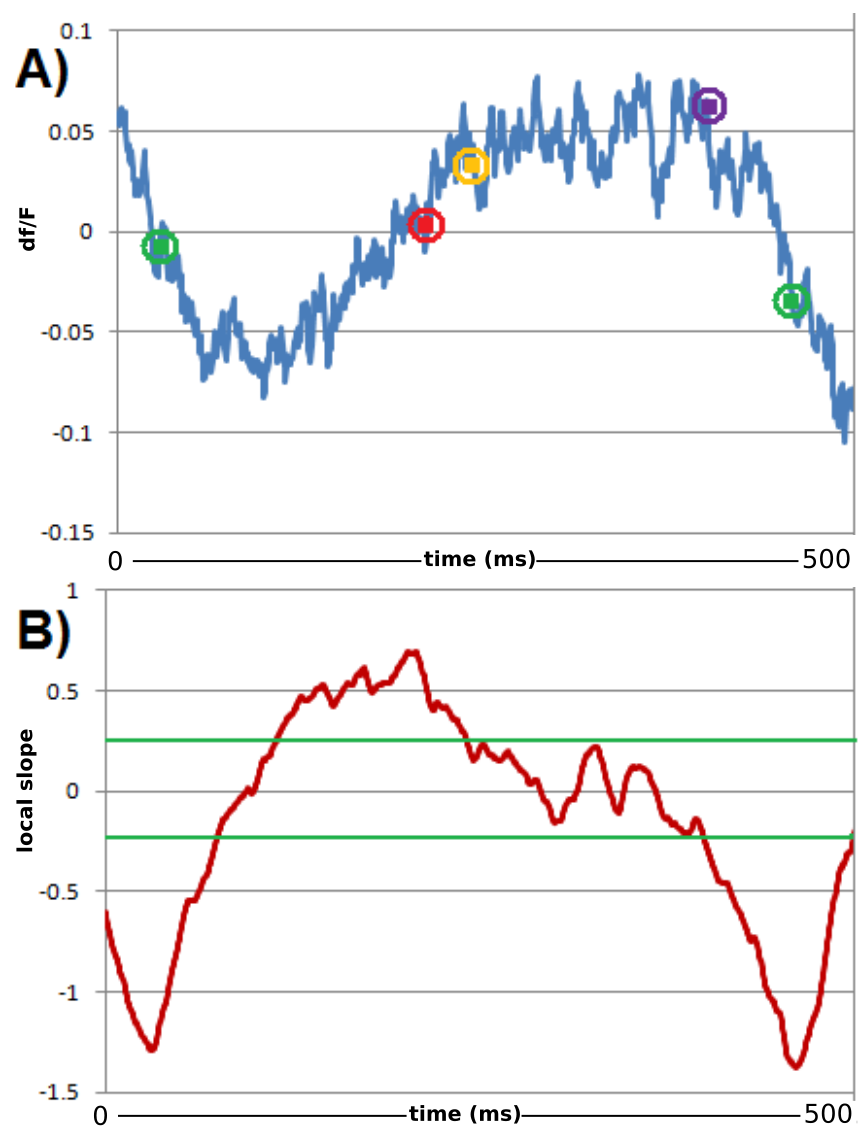
\includegraphics[width=\columnwidth]{graphics/vsd_recording.png}
		\caption[Calculated salient features shown on \ac{VSD} recording.]{\textbf{Calculated salient features shown on \ac{VSD} recording.} \Acp{VSD} recording of a PY neuron together with the minimum (green) and maximum slope (red) points and beginning (yellow) and end (purple) points  of the activity plateau determined from the data; B) The calculated local slope values, the green horizontal lines indicate the band of values considered to correspond to the activity plateau following the maximum local slope point. The horizontal axis is time in both cases and the vertical axis is voltage in arbitrary units in A) and the local slope value in B).}
		\label{fig:vsd_recording}
	\end{center}
\end{figure}

In total 11 pairs of \ac{PY} neurons from four \ac{STG} preparations (two using dye filling and two using bath application of the dye) were considered (see table \ref{tab:experiments}). The mean values and standard deviations of the temporal delays were calculated. It was found that the standard deviation of the temporal delays changed significantly in half of the cases (according to the F-test) following the application of the \ac{DA} containing saline. Results are shown in table \ref{tab:da_results} and figure \ref{fig:da_results}. In 22 cases of 44 comparisons of standard deviations it was found that the standard deviations are significantly larger following the effect of the \ac{DA} on the neurons. In one case it was found that the calculated standard deviation was significantly lower following the \ac{DA} exposure, and in the remaining 21 cases the difference between the standard deviations was not statistically significant. The lack of statistical significance means that the exposure to \ac{DA} did not have an effect on the standard deviation of temporal differences between the corresponding maximum and minimum slope points and beginning and end points of activity plateaus of pairs of \acp{PY}. The increase of the standard deviation of the temporal differences implies reduction of the temporal locking of the \acp{PY}, or in other words, the de-synchronisation of \acp{PY}. The expectation of the de-synchronisation effect of \ac{DA} on the \acp{PY} is thus confirmed.

\begin{table}
	\small
	\caption[Neuron pair comparisons.]{\textbf{Neuron pair comparisons.} In total 11 pairs of \ac{PY} neurons from four \ac{STG} preparations were considered. Two experiments used dye filling and two were bath applications. For each experiment the neurons were compared under control and \ac{DA} conditions. Using the F-test a p-value was obtained for each of the four features, thus giving the 44 values as in table \ref{tab:da_results}}.
	\label{tab:experiments}
	\begin{tabular}{llll}
		\hline
		\textbf{Experiment} & \textbf{Comparison 1} & \textbf{Comparison 2} & \textbf{Comparison 3} \\ 
		\hline
		1 (dye filling) & PY1 with PY2 & - &PY2 with PY3\\
		2 (dye filling) & PY1 with PY2 & PY1 with PY3 &PY2 with PY3\\
		3 (bath application) & PY1 with PY2 & PY1 with PY3 &PY2 with PY3 \\
		4 (bath application) & PY1 with PY2 & PY1 with PY3 &PY2 with PY3 \\
		
		\hline
	\end{tabular}
\end{table}

The suggested approach offers a way to quantify the extent of de-synchronisation of \acp{PY} in response to exposure to \ac{DA}. The presented analysis of \acp{PY} demonstrates that the methodology proposed, can be applied successfully to analyse the dynamics of temporal relationships of neural activities using optical imaging data.

\begin{table}[H]
	\small
	\centering
	\caption[Results of the \ac{DA} experiments.]{\textbf{Results of the \ac{DA} experiments.} p-values of the F-test comparisons of the temporal delay standard deviations. Significant values are shown in red.}
	\label{tab:da_results}
	\begin{tabular}{p{30mm} p{30mm} p{30mm} p{20mm}}
		\hline
		\textbf{Maximum} & \textbf{Minimum} & \textbf{Plateau} & \textbf{Plateau} \\
		\textbf{Slope Points} & \textbf{Slope Points} & \textbf{Begin Points} & \textbf{End Points} \\
		\hline
		
		0.657721015 & 0.936337338 & 0.417005168 &  0.986805014 \\
		\textcolor{red}{0.010577057} & 0.064029034 & 0.097578139 & 0.317799703 \\
		\textcolor{red}{0.000196868} & 0.303675632 & \textcolor{red}{0.066103149} & \textcolor{red}{0.019539292} \\
		\textcolor{red}{2.66550x${10^{-19}}$} & \textcolor{red}{4.10299x${10^{-06}}$} & \textcolor{red}{2.01957x${10^{-15}}$} & \textcolor{red}{0.000686408} \\
		\textcolor{red}{7.86896x${10^{-19}}$} & \textcolor{red}{9.69148x${10^{-05}}$} & \textcolor{red}{2.93382x${10^{-15}}$} & \textcolor{red}{0.001116038} \\
		\textcolor{red}{2.92339x${10^{-26}}$} & \textcolor{red}{8.04271x${10^{-09}}$} & \textcolor{red}{8.07804x${10^{-27}}$} & \textcolor{red}{3.30665x${10^{-15}}$} \\
		0.729215365 & 0.637028887 & 0.841677533 & 0.687908256 \\
		0.734146578 & 0.411370955 & 0.302637642 & 0.819808126 \\
		\textcolor{red}{6.67436x${10^{-05}}$} & 0.263113108 & \textcolor{red}{0.006803160} & \textcolor{red}{ 0.000531943} \\
		0.665538015 & \textcolor{red}{0.024729645} & 0.976871651 & 0.131110278 \\
		\textcolor{red}{0.018054682} & \textcolor{red}{0.002703960} & 0.285120361 & \textcolor{red}{0.004076710} \\
		\hline
	\end{tabular}
\end{table}

\begin{figure}[H]
	\begin{center}
		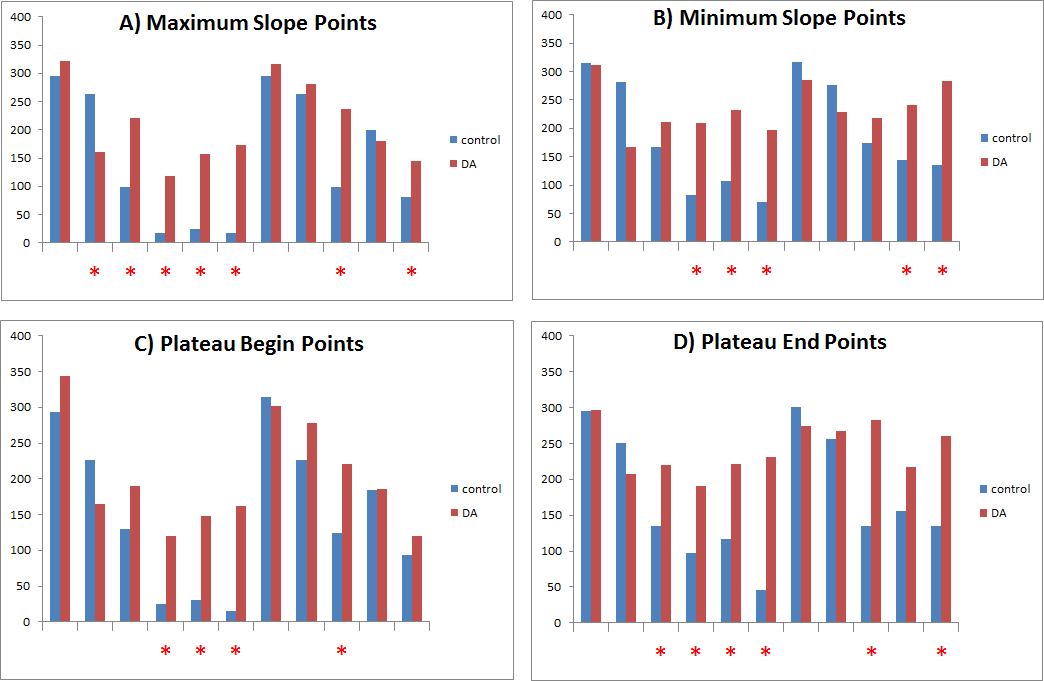
\includegraphics[width=\columnwidth]{graphics/da_results.png}
		\caption[The results of the \ac{DA} experiments.]{\textbf{The results of the \ac{DA} experiments.} The calculated standard deviation values are shown on the vertical axes. Each pair of bars represents a comparison of a pair of \ac{PY} neurons. Comparisons that resulted in a significant p-vale (\textless 0.05) are indicated by a red asterisk on the horizontal axis. The p-values were calculated using the F-test and are given in table \ref{tab:da_results}. PRE indicates standard deviation values calculated before the exposure to dopamine, DA indicates standard deviation values calculated following the exposures to dopamine.}
		\label{fig:da_results}
	\end{center}
\end{figure}

\note{1.7 actual vsd recording of PY neurons. wolfgang 9 may 2011 
	april 2011, 3 data set from aug, sep 2011
	1.8 result of analysis, bar chart showing the effect of the dopamine - the standard deviations are different - using the f-test.}

\section{Discussion and Conclusions}
\label{sec:analysis_discussion}
It is of vital importance that neural circuits are adaptive and flexible in the delivery of their functionality. Such flexibility relies on the dynamics of the temporal relationship between the neurons forming those neural circuits. The recording of many synaptically connected neurons, at individual neuron resolution, has not been possible under physiologically realistic conditions until relatively recently. However, current optical recording techniques using voltage sensitive dyes and calcium dyes allow high spatio-temporal resolution recordings to be made of many neurons.  Such techniques enable us to study the dynamics of temporal relationships of neural activities in biological neural circuits.

In this chapter a method was proposed for the analysis of optical data for understanding the dynamics of the temporal relationship of the activities of individual neurons. The proposed method relies on the robust identification of salient points of the activity patterns of individual neurons, such as the minimum and maximum slope points and the beginning and end points of depolarisation plateaus (the latter two only in appropriate cases). The method is very important because it allows robust analysis of optical neuro-imaging data to determine activity phases of neurons and on the basis of this, allows the quantification and analysis of the dynamics of activity patterns of multiple neurons. Other methods based on the calculation of average measurements are less robust than the method proposed. This kind of analysis is key for the understanding of the emergent functionality of neural systems. Consequently the method proposed here improves the reliability of the use of optical imaging data for this kind of analysis. The proposed method of analysis was applied to neurons recorded in the crab \ac{STG} and it was shown that, as expected, there is a statistically significant, measurable de-synchronisation effect of \ac{DA} on the considered \ac{PY} neurons. This is the first time this effect is shown in the physiologically realistic setting of the \ac{STG}, i.e. previous measurements implying this result were made in the presence of neurotoxic substances to achieve pharmacological isolation of neurons. As noted above the described method is expected to work at best in the case of neurons for which the depolarisation plateau means a larger change in the recorded membrane potential than the spikes themselves. However, it is also expected that the method should work well even for neurons where this is not the case (e.g. neurons of the mammalian cortex). In the case of these neurons the determination of minimum and maximum slope points is feasible and these allow the robust measurement of the dynamics of the temporal relationships of the activity patterns of these neurons using optical imaging data. As shown above, the proposed method works off-line. However, it is possible at least in principle to extend it to an on-line application, if the proposed analysis method is integrated with the recording of the data. With sufficiently fast processors such integration should not represent a major technical challenge. If the method is applied on-line its application is only limited by the time window required for the calculations (consider in particular the case of forward slope calculation), however even this constraint can be mitigated by considering a predictive application of the methodology (e.g. predicting the timing of salient points on the basis of previously
determined salient points and correcting the predictions when the required data becomes available). This kind of on-line application of the methodology would allow setting of additional stimulation of selected neurons depending on the activity pattern phase of measured neurons. This would make possible the design of more elaborated experiments involving measurement and experimental modulation of
the activity of multiple neurons. The method described in this chapter is also applicable to other kinds of noisy biological recordings where robust quantification of key transitions and the measurement of relative transition dynamics across multiple processes is required.
As shown, the calculation of local slope values is more robust than the
calculation of usual averages and this difference in robustness of calculations may be critically important in the context of estimation of activity pattern features from noisy recordings. For example, such cases may include other neural systems (e.g. phase determination of swim pattern generators in leeches or snails) or recordings from muscles (e.g. heart muscles or muscles involved in rhythmic movement or
swimming).

The question now remains whether it is possible to produce a computational model that will reflect the de-synchronisation that was observed. In the next chapter (chapter \ref{chap:modelling}) such a model is discussed. %Methods and Materials
	\chapter{Modelling the impact of dopamine on PY neurons}
\label{chap:modelling}
\section{Introduction}
\label{sec:model}

The Hodgkin-Huxley model is a conductance based, mathematical model that describes how action potentials in neurons are initiated and propagated. The model comprise four differential equations that were described in detail in Chapter \ref{chap:background} section \ref{sec:hogkin_huxley_model}. The original model included only potassium, sodium and leak currents. However, the model is relatively easily extensible to include several more channels and can also be adapted to create multi-compartmental representations of neurons. Each compartment is modelled with its own set of differential equations. The major challenge with this approach is the selection of parameter values and ranges finding a differential equation solver that can cope with the stiffness of the equations. Individual neuron models can be connected through model synapses to create a circuit.

\section{The Model}

In this chapter an implementation of the Hodgkin-Huxley model is presented to include five \acp{PY}, two \acp{PD}, one \ac{AB} and one \ac{LP} (fig. \ref{fig:HH_model}). Each of the neurons is modelled with two compartments, one representing the primary neurite and dendrites (A) and the other representing the soma (S) (fig. \ref{fig:two_compartment}). The A compartments are responsible for producing action potentials while the S compartments produce slow wave oscillations. 

The model has been implemented in \matlab, using the ode45 method which is based on an explicit Runge-Kutta (4,5) formula. Several of the differential equation solvers available in \matlab were tested but ode45 was the only method that would not diverge to infinity. Simulations were performed on PCs with Linux and Windows operating systems as well as on a high performance cluster.

\matlab, R and Neuron were evaluated for creating the model. The decision to use \matlab was made because Neuron was found to diverge to infinity after only a few seconds of simulation with only a simplistic model and in R all ode solvers were tested but were also found to diverge to infinity and no results could be obtained. 

\begin{figure}[H]
	\begin{center}
		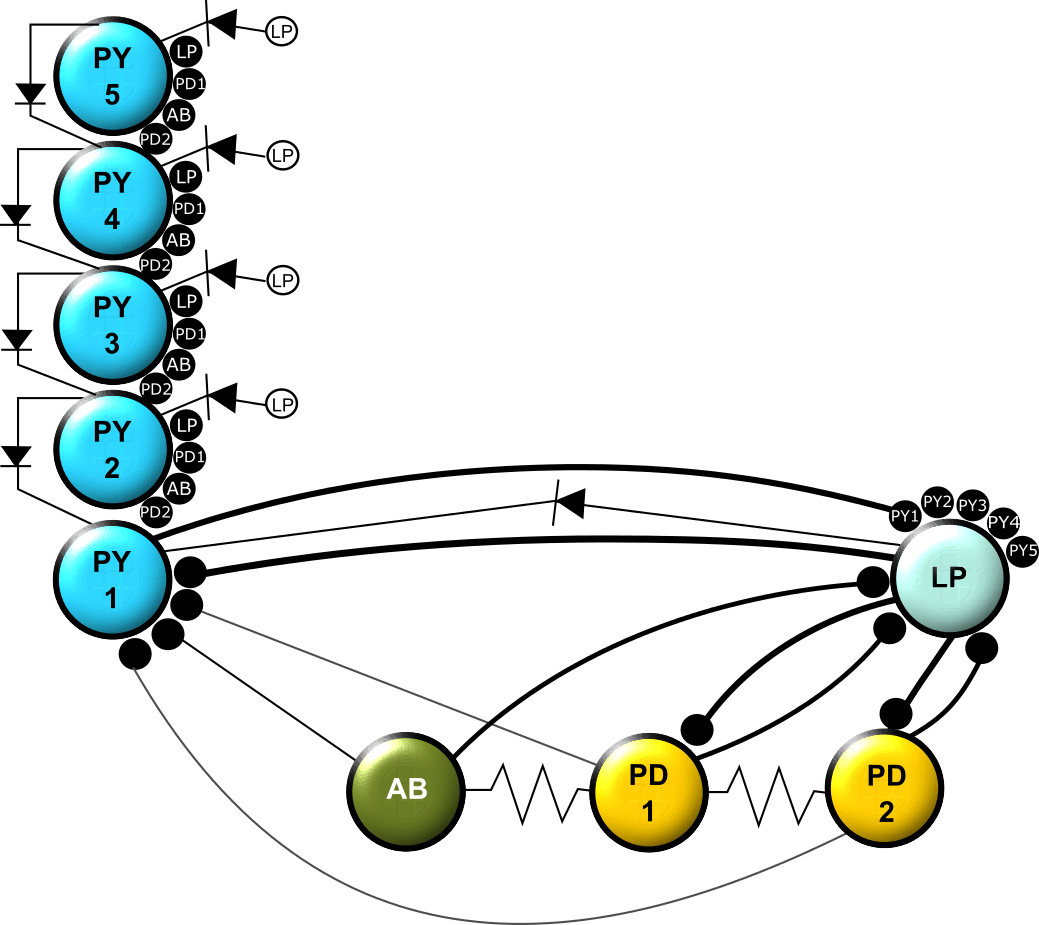
\includegraphics[width=10cm]{graphics/HH_model.png}
		\caption[Neural circuit of the pyloric \ac{CPG}.]{\textbf{Neural circuit of the pyloric \ac{CPG}. }The neural circuit of the model includes five \acp{PY}, two \acp{PD}, one \ac{AB} and one \ac{LP}. Neurons are shown with large coloured circles. All known inhibitory and electrical synapses are included in the model. The inhibitory synapses are shown as small black circles. Rectifying gap junctions are shown as diode symbols and non-rectifying gap junctions are indicated with resistor symbols. For clarity not all synapses and gap junctions in diagram are connected but the name of the inhibiting neuron is shown in the black circle. Similarly, not all the electrical synapses are connected but the name of the originating neuron is shown in a clear circle.}
		\label{fig:HH_model}
	\end{center}
\end{figure}

\begin{figure}[H]
	\begin{center}
		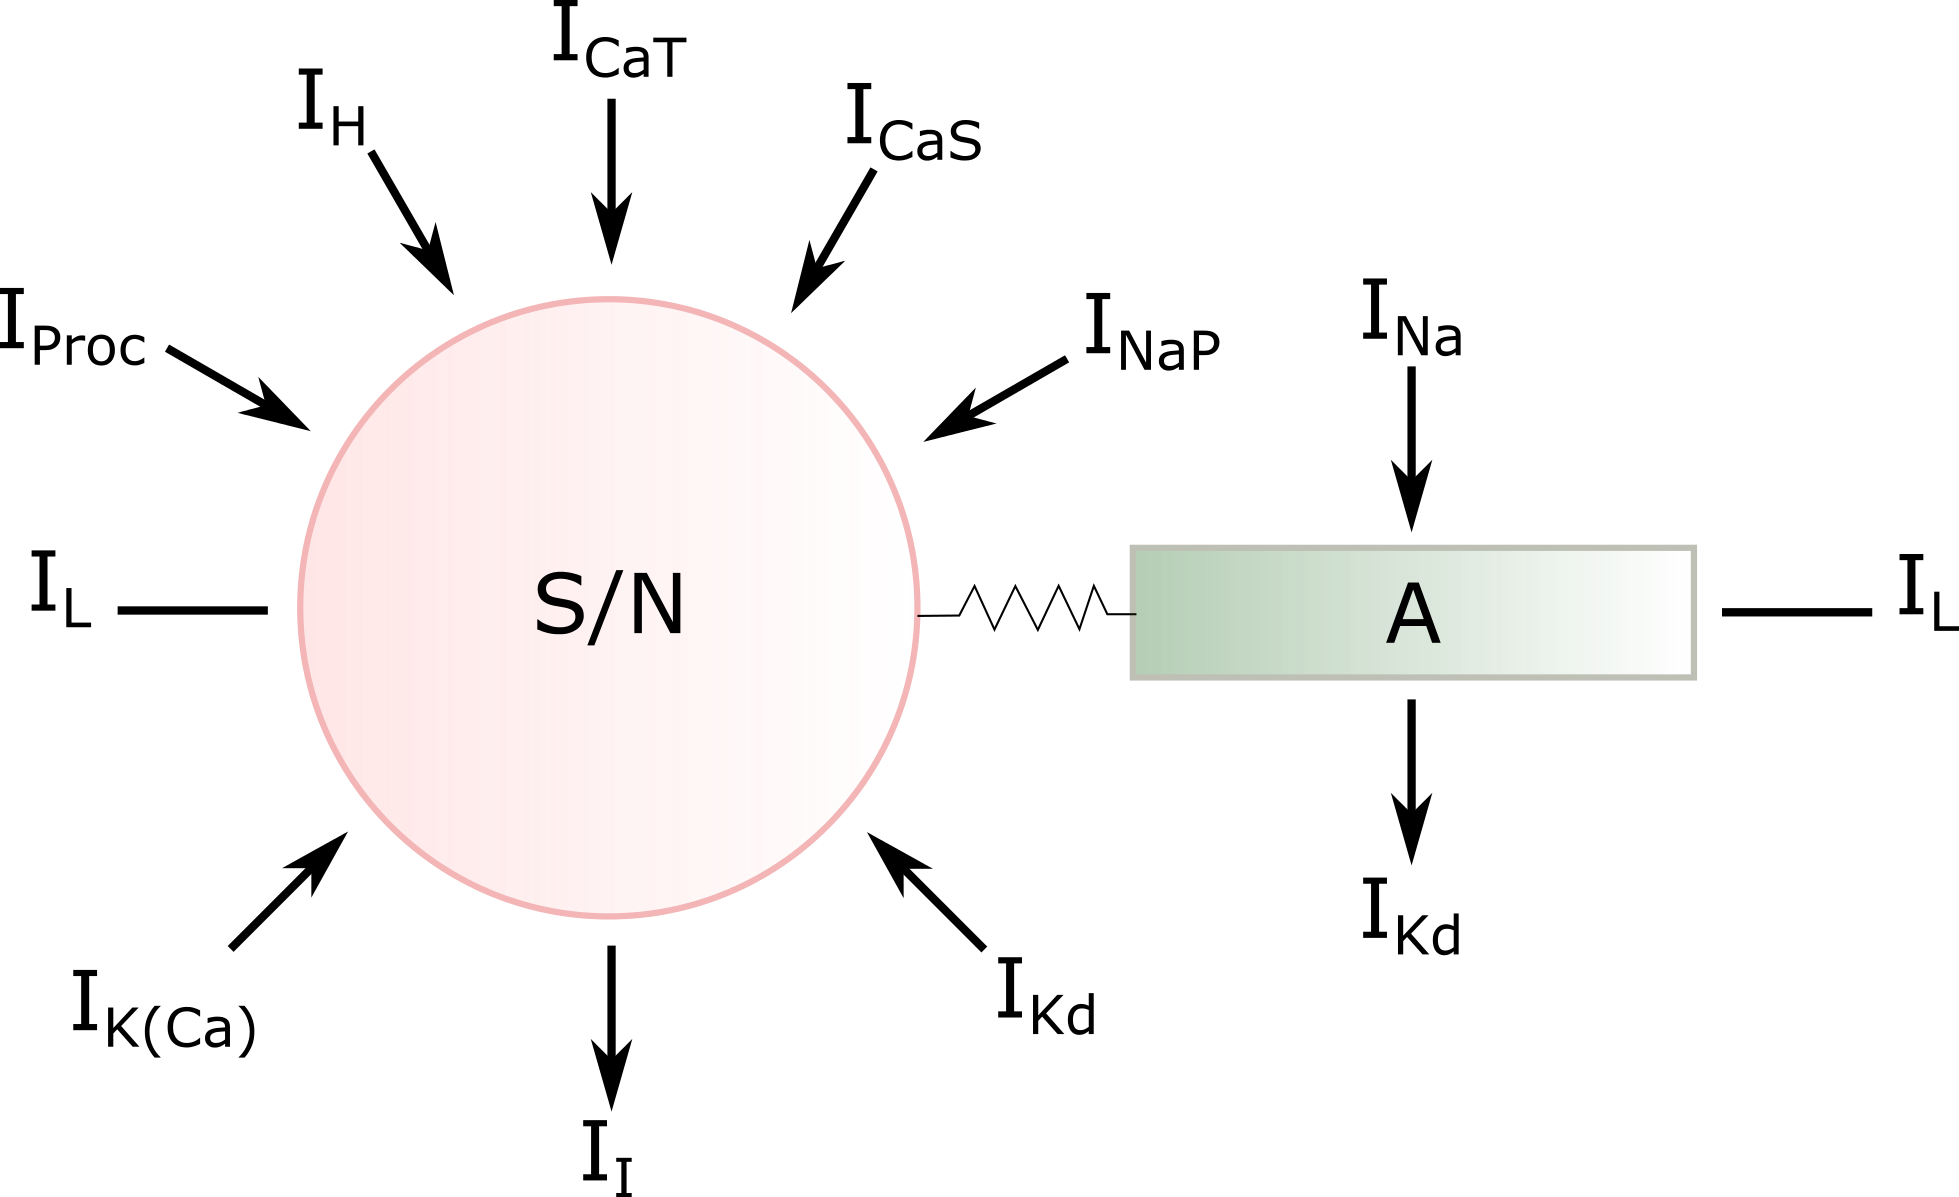
\includegraphics[width=8cm]{graphics/two_compartment.png}
		\caption[Two compartment model of a neuron.]{\textbf{Two compartment model of a neuron.} Each neuron is modelled with two compartments, S/N representing the soma and primary neurite and A representing the axon. }
		\label{fig:two_compartment}
	\end{center}
\end{figure}


\section{Parameters}
Parameters for the model was obtained from literature. For the \ac{AB} and \ac{PD} neurons the parameters were taken from research by Soto-Trevi\~{n}o \cite{Soto-Trevino2005}. The distinct intrinsic and dynamic properties of these two neurons were taken into account by using measurements from cultured \ac{STG} neurons in research performed by Turrigiano \textit{et al.} \cite{Turrigiano1995} The parameters for the \ac{LP} and \acp{PY} were adapted from Golowasch \textit{et al.} \cite{Golowasch1999a}.

\renewcommand{\tablename}{Table}
\begin{table}[H]
	\centering
	\tiny
	\caption{Parameter values of the model axons. Conductances ($g$) are in $mu S$ and reversal potentials ($E$) in $mV$.}
	\label{tab:modelparameters1}
	\begin{tabular}{ l l r l r l r l r}
		\hline
		\bf Channel & \multicolumn{2}{c}{\bf AB axon} & \multicolumn{2}{c}{\bf PD axon} & \multicolumn{2}{c}{\bf LP axon}& \multicolumn{2}{c}{\bf PY axon}\\ 
		\hline
		 & $g$ & $E$ & $g$ & $E$ & $g$ & $E$& $g$ & $E$\\ 
		\hline
		$I_{Na}$& $300e^{-3}$ & 50 \vline& $1,110e^{-3}$ & 50 \vline& $0.03e^{-3}$ & 20 \vline& $0.03e^{-3}$ & 20 \\ 
		$I_{K}$& $52.5e^{-3}$ & -80 \vline& $150e^{-3}$ & -80 \vline& $4e^{-3}$ & -80 \vline& $4e^{-3}$ & -80 \\
		$I_{L}$& $0.0018e^{-3}$ & -60 \vline& $0.00081e^{-3}$ & -55 \vline& $0.0075e^{-3}$ & -68\vline& $0.0075e^{-3}$ & -68\\
		\hline
	\end{tabular}
\end{table}

% Table generated by Excel2LaTeX from sheet 'Sheet1'
\begin{table}[H]
	\centering
	\tiny
	\caption{Parameter values of the model somas. Conductances ($g$) are in $/mu S$ and reversal potentials ($E$) in $mV$.}
	\label{tab:addlabel}%
	\begin{tabular}{llrlrlrlr}
		\hline
		\bf Channel & \multicolumn{2}{c}{\bf AB soma} & \multicolumn{2}{c}{\bf PD soma} & \multicolumn{2}{c}{\bf LP soma} & \multicolumn{2}{c}{\bf PY soma} \\
		 & g & e & g & e & g & e & g & e \\
		\hline
		$I_{Na}$  & $2.7e^{-3}$ & 50 \vline& $4.383^{-3}$ & 50 \vline& \centering\textemdash & \textemdash \vline& \textemdash & \textemdash \\
		$I_{H}$  & $0.054e^{-3}$ & -20 \vline& $0.219e^{-3}$ & -20 \vline& $0.005e^{-3}$ & -20 \vline& $0.005e^{-3}$ & -20 \\
		$I_{K}$  & $1890e^{-3}$ & -80 \vline& $1576.8e^{-3}$ & -80 \vline& $0.1e^{-3}$ & -80  \vline & $0.1e^{-3}$ & -80 \\
		$I_{KCA}$ & $6000e^{-3}$ & -80 \vline& $251.84e^{-3}$ & -80 \vline& \centering\textemdash & \textemdash \vline& \centering\textemdash &  \textemdash \\
		$I_{A}$  & $21.6e^{-3}$ & -80 \vline& $39.42e^{-3}$ & -80 \vline& $0.01e^{-e}$ & \textemdash \vline& $0.025e^{-3}$ & \textemdash \\
		$I_{P}$  & $570e^{-3}$ & 0 \vline& 0  & 0  \vline& $0.04e^{-3}$ & -10 \vline& 0  & -10 \\
		$I_{L}$  & $0.045e^{-3}$ & -50 \vline& $0.105e^{-3}$ & -55 \vline& $0.025e^{-3}$ & -68 \vline& $0.015e^{-3}$ & -68 \\
		$I_{CaT}$ & $55.2e^{3}$ & \textemdash \vline& $22.5e^{-3}$ & \textemdash \vline& \centering\textemdash & \textemdash \vline& \textemdash & \textemdash \\
		$I_{CaS}$ & $9e^{-3}$ & \textemdash \vline& $60e^{-3}$ & \textemdash \vline& \centering\textemdash & \vline & \textemdash & \textemdash \\
		$I_{Ca}$ & \centering\textemdash & \textemdash \vline& \centering\textemdash & \textemdash \vline& $0.1e^{-3}$ & 120 \vline& $0.1e^{-3}$ & 120 \\
		\hline
	\end{tabular}%
\end{table}%

\section{Equations}

Mathematically the currents for gap junctions ($I_{gap}$) and couplings between the S/N and A compartments are described with the same equation. Coupling currents in the coupled compartments are symmetric, thus the coupling current between the soma and the axon would be:

\begin{equation}
\label{eq:coup}
I_{axial_{S/N}} = -I_{axial_{A}}
\end{equation}

and the gap junction between neurons $i$ and $j$ would be:

\begin{equation}
\label{eq:gap}
I_{gap_{i}}=-I_{gap_{j}}
\end{equation}

For each of the S/N compartments the axial current is the product of the axial conductance and the difference of the membrane potential in the A and S/N compartments:

\begin{equation}
\label{eq:axial_conductance}
I_{axial_{S/N}} = g_{axial}(V_{S/N} - V_{A})
\end{equation}

Gap junctions use a similar equation where the conductance $I_{gap_{i}}$ is the product of the gap-junctional conductance and the membrane voltage difference between the two S/N compartments of neurons $i$ and $j$:

\begin{equation}
\label{eq:gap_conductance}
I_{gap_{i}} = g_{gap}(V_{S/N_{i}} - V_{S/N_{j}})
\end{equation}

In all compartments the conservation of current is represented by the partial differential equation of the form:

\begin{equation}
C\frac{dV}{dt} = I_{ext} - I_{int} - I_{coup}
\end{equation} 

and 

\begin{equation}
C\frac{dV}{dt} = I_{ext} - I_{int} - I_{gap}
\end{equation} 


where:

$C$ is the membrane capacitance.

$I_{ext}$ is the externally injected current.

$I_{int}$ is the sum of all modulatory and intrinsic currents.

$I_{coup}$ is the sum of the axial current of the adjacent compartment. 

$I_{gap}$ is the gap junctional current in the case of the S compartment.

Each of the currents is described in terms of maximal conductance and voltage-dependant gating variables:

\begin{equation}
I_{i} = g_{i}m_{i}^{pi}h_{i}^{qi}(V-E_{i})
\end{equation}

where:

$g_{i}$ is the maximal conductance.

$m_{i}$ is the activation current.

$h_{i}$ is the inactivation current.

$p_{i}$ and $q_{i}$ depends on the current type and takes integer values between zero and four.

$E_{i}$ is the reversal potential for ion ${i}$.

The behaviour of the activation and inactivation currents are modelled with the following equations:

\begin{equation}
	\label{eq:activation}
	\tau_{m}(V)\frac{dm}{dt} = m_{\infty}(V)-m
\end{equation}

\begin{equation}
	\label{eq:inactivation}
	\tau_{h}(V)\frac{dh}{dt}=h_{\infty}(V)-h
\end{equation}

where:

$m_{\infty}$ and $h_{\infty}$ are steady-state values.

$\tau_{m}$ and $\tau_{h}$ are time constants.

Table \ref{tab:gates} and \ref{tab:gates2} gives the dependency of voltage and intracellular $Ca^{2+}$ concentrations for each of these functions. The steady-state activation of $I_{KCa}$ is also dependent on $[Ca^{2+}]$ and provided in table \ref{tab:gates}.

The values of the exponents $p_{i}$ and $q_{i}$ are dependent on the current type and takes a value between 0 and 4.

The calcium activated potassium channels ($KCa$) of \ac{AB} and \ac{PD} are critical for their roles as pacemakers in the pyloric circuit. These channels only occur in the S/N compartments of the \ac{AB} and \ac{PD} and not in any of the other neurons. $Ca^{2+}$ is governed by the following equation:

\begin{equation}
\label{eq:KCa_concentration}
\tau_{Ca}\frac{d[Ca^2+]}{dt}-FI_{Ca}-[Ca^{2+}] + C_{0} 
\end{equation}

where:

$\tau_{Ca}$ is the $Ca^{2+}$ buffering time constant.

$C_{0}$ is the background intracellular $Ca^{2+}$ concentration.

$F$ converts the total $Ca^{2+}$ current $I_{Ca}$, in nA, into an intracellular concentration. 


The reversal potential for all currents, apart from $E_{Ca}$ are constants, given in table \ref{tab:modelparameters1}. The Nernst equation (\ref{eq:Nernst}) is used to compute the reversal potential for $E_{Ca}$, with an extracellular concentration of 13 $mM$ \cite{Buchholtz1992, Soto-Trevino2005}.

\begin{table}[H]
	\centering
	\caption{\ac{PD} and \ac{AB} voltage and calcium dependency for the steady-state activation $m$ and inactivation $h$ of the currents (adopted from \cite{Soto-Trevino2005} and \cite{Golowasch1999a})}
	\label{tab:gates}
	{\renewcommand{\arraystretch}{2}%
	\begin{tabular}{lcll}
		\hline
		& $m,h$ & $x_{\infty}$ & $\tau_{x}$,ms \\
		\hline
		% --- INa ---
		\multirow{3}{*}{ $I_{Na^{+}}$ } & $m^{3}$  & $\dfrac{1}{1+exp [ - ( V+24.7 / 5.29 ) ] }$ & $1.32 - \dfrac{1.26}{1+ exp \lbrack -( V+120 / 25 ) \rbrack}$ \\
		& $h$ & $\dfrac{1}{1 + exp [ ( V + 48.9 ) / 5.18 ]}$ & $ \Bigg\{ \dfrac{0.67}{1 + exp [ - ( V + 62.9 ) / 10] } \Bigg\} $ \\ 
		& & & $ \times \Bigg\{ 1.5 + \dfrac{1}{1 + exp [ ( V + 34.9 ) / 3.6 ] } \Bigg\} $ \\
		% --- IK ---
		$I_{K}$ & $m^{4}$ & $\dfrac{1}{ 1 + exp [ - ( V + 14.2 ) / 11.8 ]}$ & $7.2 - \dfrac{6.4}{ 1 + exp [ - ( V + 28.3 ) / 19.2] } $ \\
		% --- ICaT ---
		\multirow{3}{*}{ $ I_{CaT} $} & $m^{3}$ & $\dfrac{1}{ 1 + exp [ -( V + 25 ) / 7.2 ]}$ & $ 55 - \dfrac{49.5}{ 1 + exp [ - ( V + 48 ) / 17  ] } $ \\
		& $h$ & $ \dfrac{1}{ 1 + exp [ ( V + 36 ) / 7 ] } $ & AB:$ 87.5 - \dfrac{75}{ 1 + exp [ - ( V + 50 ) / 16.9 ] } $\\
		& & & PD:$ 350 - \dfrac{300}{ 1 + exp [ - ( V + 50 ) / 16.9] } $ \\
		% --- ICaS ---
		$ I_{CaS} $ & $ m^{3} $ & $ \dfrac{1}{ 1 + exp [ - ( V + 22) / 8.4 ] } $ & $ 16 - \dfrac{13.1}{ 1 + exp [ - ( V + 25.1 ) / 26.4 ] } $ \\
		% --- INap ---
		\multirow{2}{*}{ $ I_{Nap} $ } &  $ m^{3} $ & $ \dfrac{1}{ 1 + exp [ - ( V + 26.8 ) / 8.2 ] } $ & $ 19.8 - \dfrac{10.7}{ 1 + exp [ - (V + 26.5 ) / 8.6 ] } $ \\
		& $ h $ & $ \dfrac{1}{ 1 + exp [ ( V + 48.5 ) 4.8 ] } $ & $ 666 - \dfrac{379}{ 1 + exp [ - ( V + 33.6 ) / 11.7 ] }$ \\
		% --- h ---
		$ I_{h} $ & $ m $ & $ \dfrac{1}{ 1 + exp [ ( V + 70 ) / 6 ] } $ & $ 272 + \dfrac{1499}{ 1 + exp [ - ( V + 42.2 ) / 8.73 ] } $ \\
		% --- KCa ---
		% ----------- AB
		\multirow{2}{*}{ $I_{KCa}$ } & \multirow{2}{*}{ $m^{4}$ } & AB:$ \Bigg( \dfrac{ [ Ca ] }{ [ Ca ] + 30 } \Bigg) \times $ &  $ 90.3 - \dfrac{75.09}{ 1 + exp [ - ( V + 46 ) / 22.7] } $\\
		& & $\dfrac{1}{ 1 + exp [ - ( V + 51 ) / 4 ] } $ & \\
		% ----------- PD
		& & PD: $ \Bigg( \dfrac{ [ Ca ] }{ [ Ca ] + 30 }\Bigg) \times $ & \\
		& & $\dfrac{1}{ 1 + exp ([ - ( V + 51 ) / 8 ]) } $ & \\
		% --- IA ---
		\multirow{3}{*}{ $ I_{A} $ }& $ m^{3} $ (AB) & \multirow{2}{*}{$ \dfrac{1}{ 1 + exp [ - ( V + 27 ) / 8.7 ]}$} & \multirow{2}{*}{$ 11.6 - \dfrac{10.4}{ 1 + exp [ - ( V + 32.9 ) / 15.2 ] } $} \\
		& $m^{4}$ (PD) & &  \\
		& $h$ & $\dfrac{1}{ 1 + exp [ ( V + 45.9 ) / 4.9 ] } $ & $ 38.6 - \dfrac{29.2}{ 1 + exp [ - ( V + 38.9 ) / 26.5 ] }$ \\ 
		$I_{proc}$ & $m$ & $ \dfrac{1}{ 1 + exp [ - ( V + 12 ) / 3.05 ] }$ & $ 0.5 $ \\		
		\hline
	\end{tabular}
	}
\end{table}

\begin{table}[H]
	\centering
	\caption{\ac{LP} and \ac{PY} voltage and calcium dependency for the steady-state activation $m$ and inactivation $h$ of the currents (adopted from \cite{Golowasch1999a})}
	\label{tab:gates2}
	{\renewcommand{\arraystretch}{2}%
		\begin{tabular}{lcll}
		\hline
		& $m,h$ & $x_{\infty}$ & $\tau_{x}$,ms \\
		\hline
		% --- Ca ---
		\multirow{2}{*}{ $I_{Ca}$ } & $m$ & $\dfrac{1}{ 1 + exp [ 0.205 ( - 61.2 - V ) ] }$ & $ 30 + \dfrac{-5}{ 1 + exp [ 0.2 ( -65 - V ) ] } $ \\
		& $h$ & $\dfrac{1}{ 1 + exp [ -0.15 ( - 75 - V ) ] } $ & $ 150 $\\
		% --- K ---
		$I_{K}$ & $m$ & $ \dfrac{1}{ 1 + exp [ 0.1 ( -35 - V ) ] } $ & $ 2 + \dfrac{55}{ 1 + exp [ -0.125 (-54-V ) ] } $ \\
		% --- A ---
		\multirow{3}{*}{$I_{A}$} & \multirow{2}{*}{ $m$ } & PY:$ \dfrac{1}{1 + exp[ 0.2 ( -51 - V ) ] } $ & \multirow{2}{*}{$0.1$} \\
		& & LP: $\dfrac{1}{ 1 + exp [ 0.2 ( -60 - V ) ] } $ & \\
		& $h$ & $\dfrac{1}{ 1 + exp [ -0.18 ( -68 - V ) ] } $ & $50$ \\
		% --- P ---
		$I_{P}$ & $m$ & $ \dfrac{1}{1 + exp [ 0.2 ( -55 - V ) ] } $ & $6$ \\
		% --- Na ---
		\multirow{2}{*}{$I_{Na}$} & $m^{3}$ & $ \dfrac{1}{1 + exp[ 0.1 ( -42.5 - V ) ]} $ & $0.025$ \\
		& $h$ & $\dfrac{1}{1 + exp[ -0.13 * ( -50 - V ) ] } $ & $ \dfrac{10}{ 1 + exp [ 0.12 ( -77 - V ) ] } $ \\
		% ---Kd ---
		$I_{Kd} $ & $m^{4}$ & $ \dfrac{1}{ 1 + exp [ 0.2 ( -41 - V ) ] } $ & $ 12.2 + \dfrac{10.5}{1 + exp [ - .05 ( 58 - V ) ] } $ \\
		\hline
		\end{tabular}
	}
\end{table}

\subsection{Modelling the Impact of Dopamine}

\Ac{DA} differentially modulates the neurons of the pyloric network. The following combinations of variation to the $K^{+}$ channel conductances and gap junction conductances were modelled:

\begin{itemize}
\item The potassium conductances ($g_{K}$) for \acp{PY} were fixed to $10^{-4}$. Conductances for other channels were also all fixed. Gap junction conductances were varied from 0\% to 100\% of $2.7\times10^{-7}$ in increments of 10\%. 
\item Ten randomly generated potassium conductances in an initial range of $5\times10^{-5}$ to $0.2\times10^{-3}$ . Conductances of channels A and H were percentages of K (Table \ref{tab:percentages}). Gap junctions were modelled for each of the conductances at $10^{-6}$ at 100\%, 50\% and 10\%.
\item Ten randomly generated conductances in a narrower range of $9\times10^{-5}$ to $1.1\times10^{-4}$ . Conductances of channels A and H were percentages of K (Table \ref{tab:percentages}). Gap junctions were modelled for each of the conductances at $10^{-6}$, from 100\% to 0\%.
%\note{(Table \ref{tab:randomK1})}
%\item Ten randomly generated conductances in range ?. Other conductances fixed. Gap junctions at 10e-6, 50\% and 10\%
%\note{(Table \ref{tab:randomK2})}
\end{itemize}

\begin{table}{H}
	\centering
	\caption{Values for channels A and H were calculated as percentages of the potassium channels (\cite{Temporal2012})}
	{\renewcommand{\arraystretch}{2}%
	\begin{tabular}{l l}
		\hline
		\textbf{Channel conductance} & \textbf{Percentage (\%)} \\
		\hline
		gA & 0.8875 \\
		gH & 0.087 \\
		\hline
	\end{tabular}}
	\label{tab:percentages}
\end{table}

\subsection{Calculating Dyssynchrony}
\label{sec:dyssync}
After the models were run a \matlab script, findpeaks \footnote{http://terpconnect.umd.edu/~toh/spectrum/PeakFindingandMeasurement.htm}, was used to detect spikes for each of the modelled \acp{PY} (figure \ref{fig:findpeaks}). The detected spikes were then passed to another \matlab script, SPIKY \cite{Kreuz2013}\footnote{http://www.fi.isc.cnr.it/users/thomas.kreuz/Source-­‐Code/SPIKY.html.}. SPIKY uses the spike distance as a parameter-free and timescale-independent measure of spike train synchrony. SPIKY also calculates the inter-spike interval which quantifies local dissimilarities based on the neurons' firing rate profiles.  


\begin{figure}[H]
	\begin{center}
		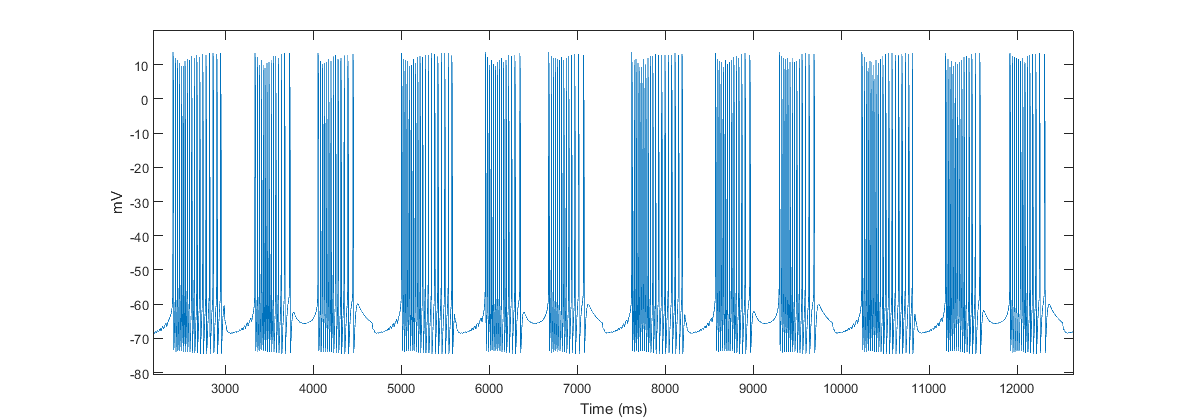
\includegraphics[width=\columnwidth]{graphics/peakfinder.png}
		\caption[findpeaks result.]{\textbf{findpeaks result.} findpeaks is a \matlab script that can detect spikes. The detected spikes are used by SPIKY to calculate spike-distance and inter-spike intervals. This plot was generated from the peaks detected by findpeaks from the output of the \matlab model. The trace represents one modelled \ac{PY} neuron. The peaks found for all the \ac{PY} neurons are passed to SPIKY which is then used to calculate \ac{ISI} and \ac{SD}}
		\label{fig:findpeaks}
	\end{center}
\end{figure}

In the next chapter the results of applying the methods discussed will be presented.

\

%\note{what is HH model
%how do you apply this to STG neurons
%where do you get parameters from - paper of ST, golowasch, harris-warrick
%how did yo get parameters py, lp, pd, ab, Temporal,
%how gap junctions model,
%how impact of da is model by changing gap junction strength.
%spiky
%}

\section{Results: The Model Output}

Traditionally \acp{PY} are modelled as one neuron implying that the same parameters are valid for all of them. However, we know that parameters vary quite widely and more recently it has also been shown that some conductance values maintain certain fixed ratios \cite{Temporal2012}. 

The variations and ratios of the parameters are implemented in our model as follows. A set of one hundred potassium conductance values were generated by using a uniform distribution over an interval. Each set consisted of five values (for the five \acp{PY}) randomly generated between of $5\times^{-5}$ to $2\times10^{-4}$. A and H channel conductances were calculated accordingly using the ratios as given in table \ref{tab:percentages}. For each of these sets, models were generated that would vary the gap junction conductance strength between zero and 100 percent of the gap junction normal strength ($10^{-6} \mu$Siemens).

For each of the models, the spike trains were detected using the \textit{findpeaks} \matlab script mentioned in section \ref{sec:dyssync}. The SPIKY \matlab script was then used to determine the \ac{ISI} and \ac{SD} for the five \ac{PY} spike trains (see figure \ref{fig:SpikeDistance}). The \ac{ISI} and \ac{SD} calculated by SPIKY are methods for quantifying the similarities in neuron's firing rate profiles and the degree of synchronisation between two spike trains on a continuous scale \cite{Kreuz2011}.

\begin{figure}[H]
	\begin{center}
		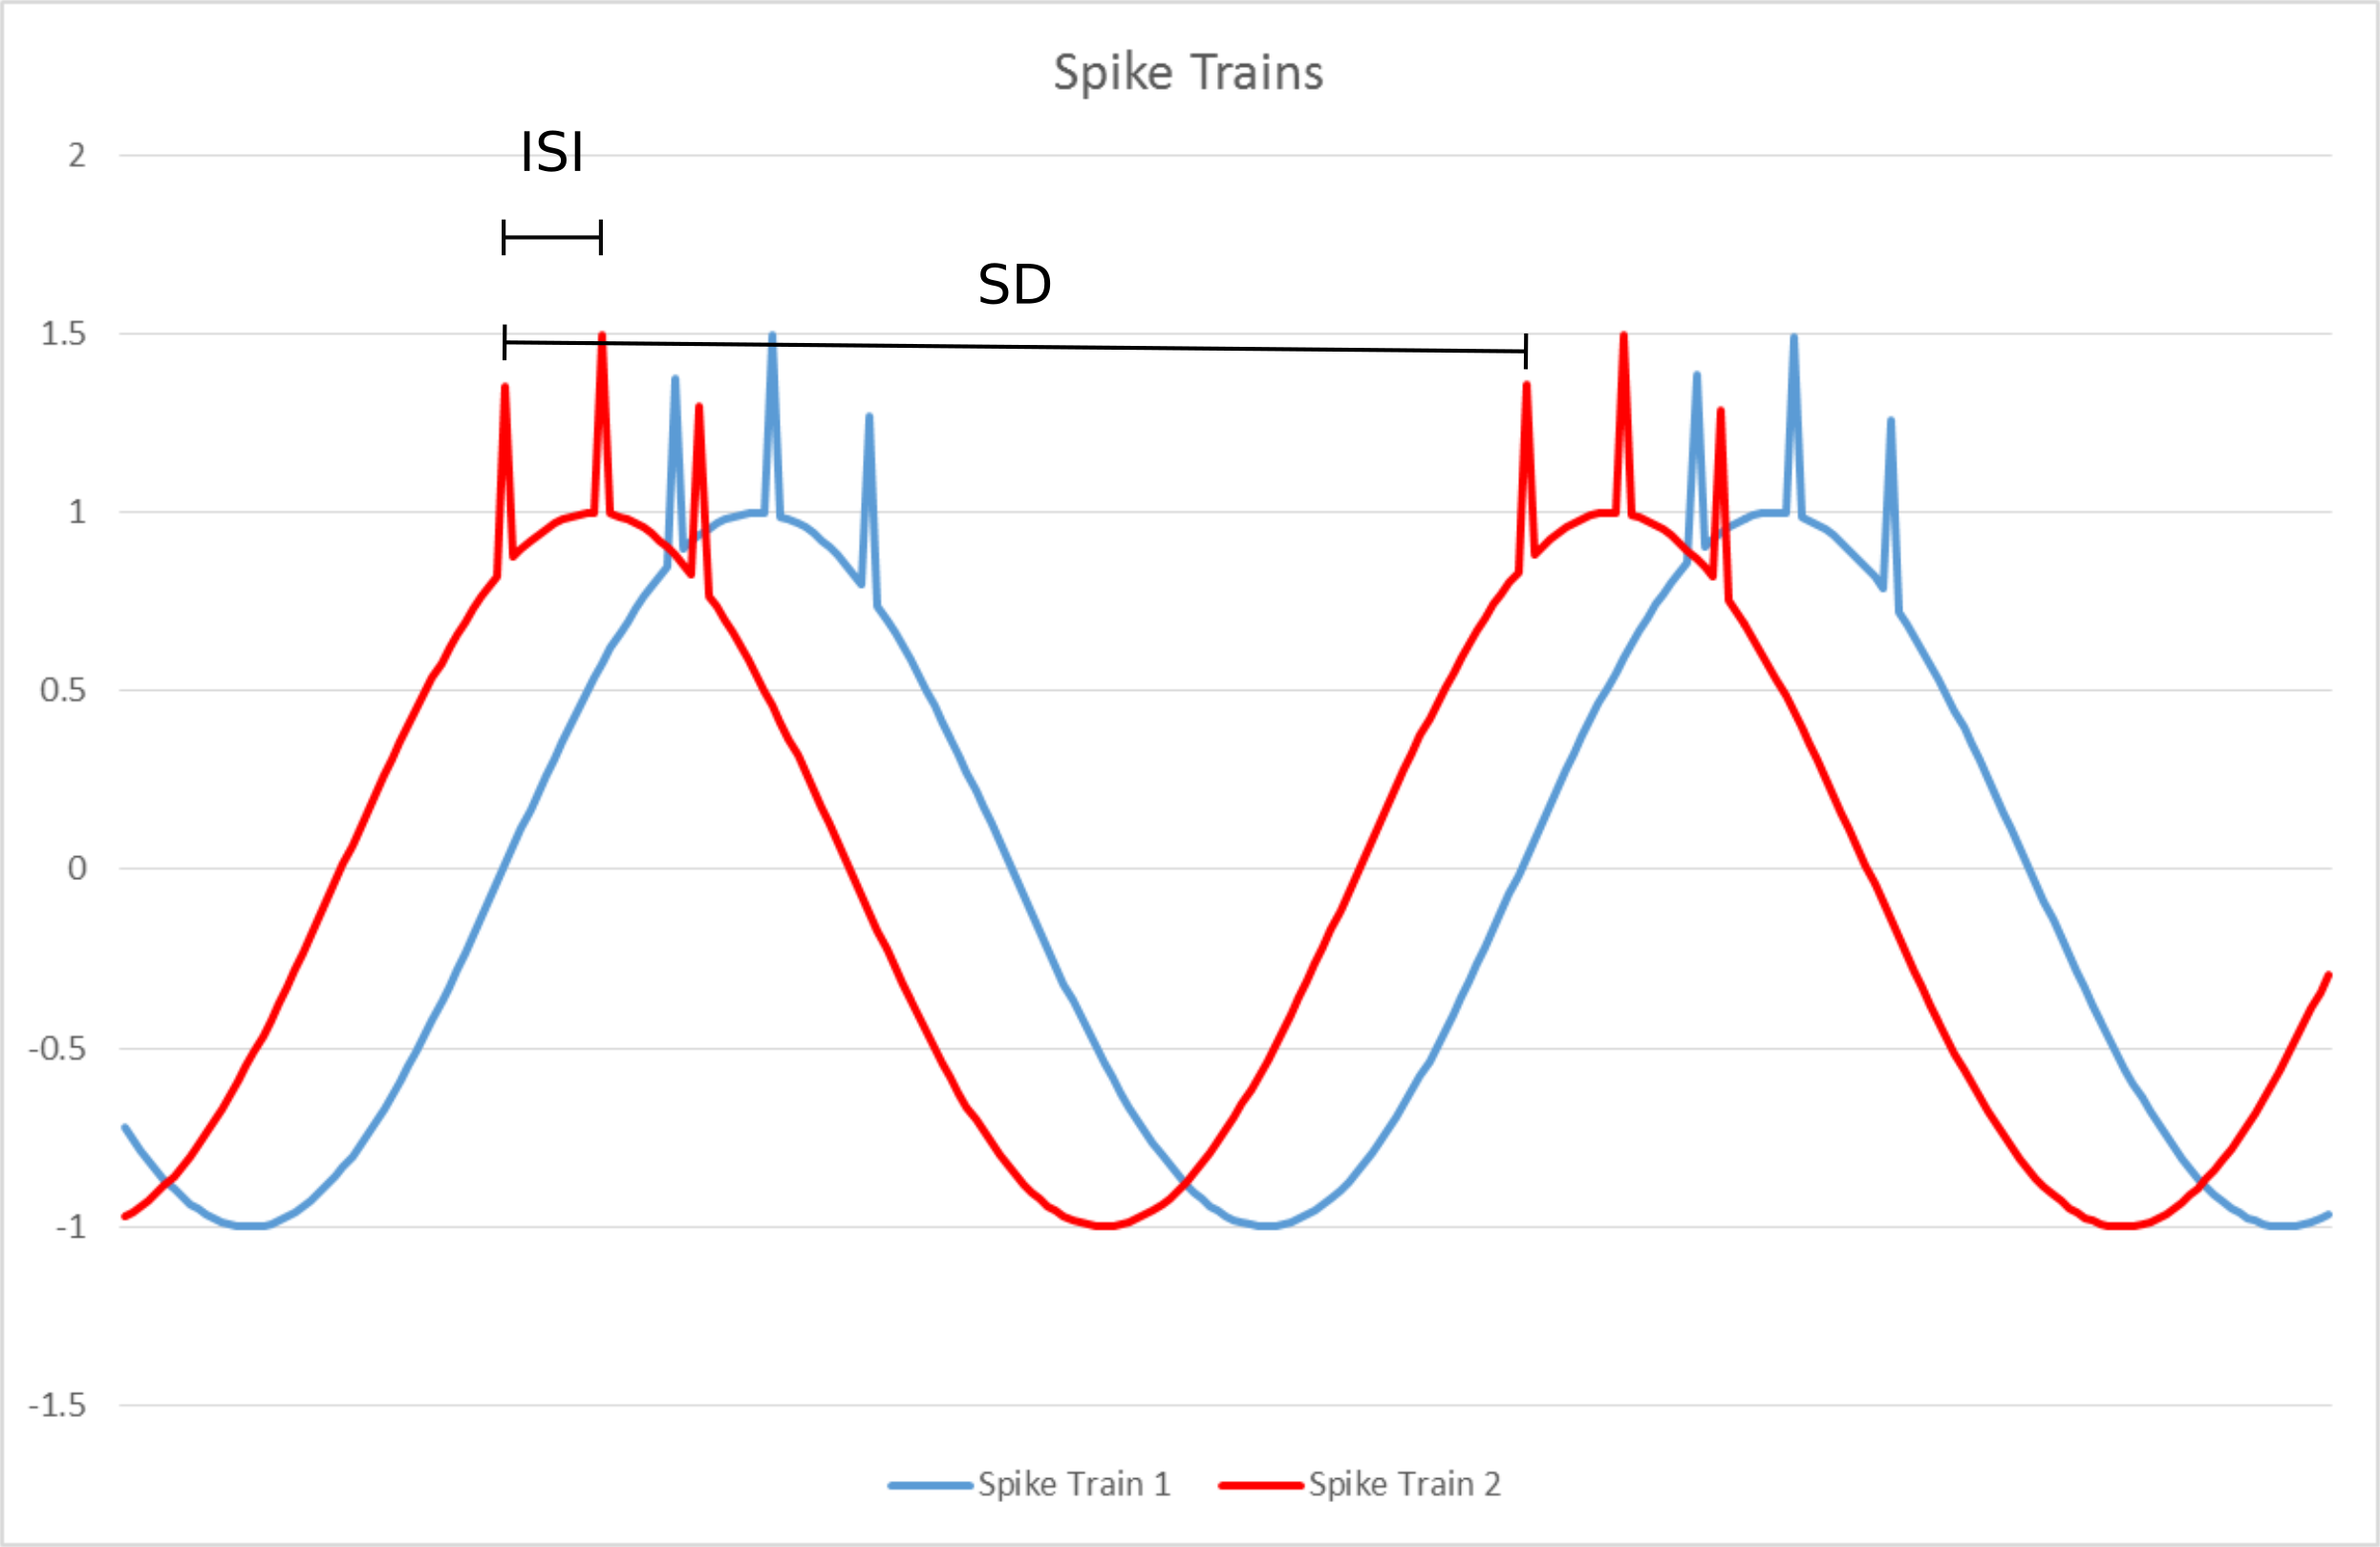
\includegraphics[width=\columnwidth]{graphics/SpikeDistance.png}
		\caption[Spike distance (SD) and inter-spike interval.]{\textbf{Spike distance (SD) and inter-spike interval.} A simplified representation of spike distance and inter-spike interval. ISI would be the distance between the spikes in a spike train. SD would be the distance between two spike trains. Detailed descriptions of exactly how these values are calculated by SPIKY can be found in the Kreuz papers \cite{Kreuz2007, Kreuz2009, Kreuz2011, Kreuz2013}}
		\label{fig:SpikeDistance}
	\end{center}
\end{figure}


Below are plots showing the effect of the changing gap junction strengths on \ac{ISI} and \ac{SD}. Figure \ref{fig:means_ISI} and \ref{fig:means_SD} plot the means of the \ac{ISI} and \ac{SD} values for each of the gap junction strength percentages. It would be expected that the stronger the gap junction conductances are, the closer the \ac{SD} would be to zero, thus more synchronised. The weaker the gap junction conductances are, the more de-synchronised the neurons are expected to be and thus the values \ac{SD} should increase. A changing \ac{ISI} indicates a change in the firing rate of a neuron.

To test the significance of any changes that might have occurred when the gap junction strength is changed, t-tests are used to test each gap junction conductance strength against the 100 percent strength. The \acp{ISI} and \acp{SD} were gathered and tested in this way for each gap junction conductance to provide a comparison measure. Figures \ref{fig:ttest_ISI} and \ref{fig:ttest_SD} show plots of the p-values from the t-tests over the gap junction strengths. The horizontal red line indicates a significance value of 0.05.

\begin{figure}[H]
	\begin{center}
		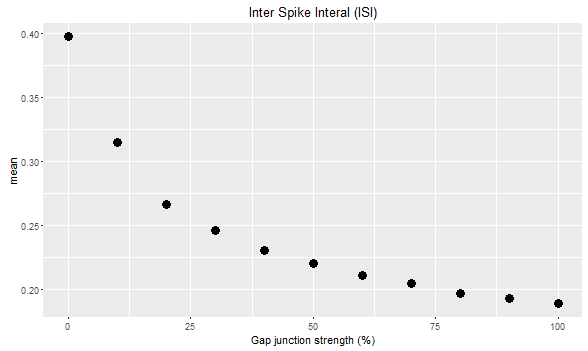
\includegraphics[width=14cm]{graphics/NewISImean.png}
		\caption[Means of inter-space interval for gap junction conductance strength.]{\textbf{Means of inter-space interval for gap junction conductance strength.}}
		\label{fig:means_ISI}
	\end{center}
\end{figure}
\begin{figure}[H]
	\begin{center}
		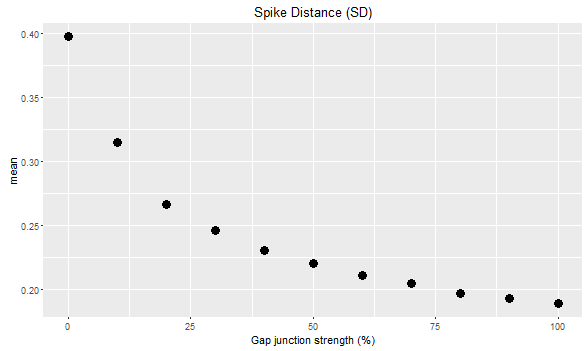
\includegraphics[width=14cm]{graphics/NewSDmean.png}
		\caption[Means of spike distance for gap junction conductance strength.]{\textbf{Means of spike distance for gap junction conductance strength.}}
		\label{fig:means_SD}
	\end{center}
\end{figure}

\begin{figure}[H]
	\begin{center}
		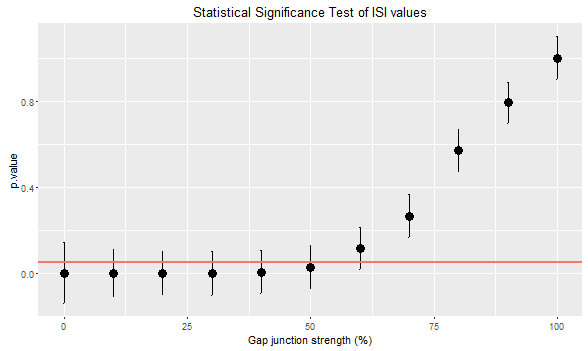
\includegraphics[width=14cm]{graphics/NewISIpvalue.png}
		\caption[Statistical Significance Test of ISI Values.]{\textbf{Statistical Significance Test of ISI Values.} The \ac{ISI} calculated for each gap junction conductance strength (from 0\% to 100\% of $10e^{-6}\mu$S) is tested against 100\% \ac{ISI}. The horizontal bars show standard deviation.}
		\label{fig:ttest_ISI}
	\end{center}
\end{figure}
\begin{figure}[H]
	\begin{center}
		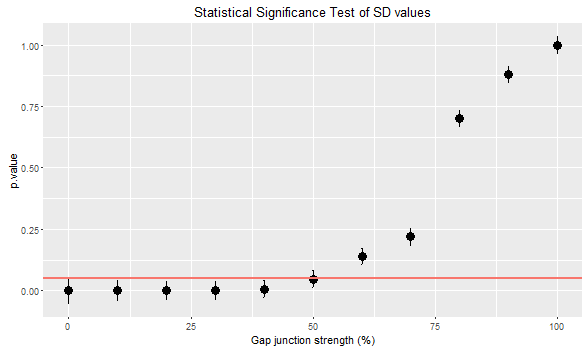
\includegraphics[width=14cm]{graphics/NewSDpvalue.png}
		\caption[Statistical Significance Test of Spike Distance Values.]{\textbf{Statistical Significance Test of Spike Distance Values.} The \ac{SD} calculated for each gap junction conductance strength (from 0\% to 100\% of $10e^{-6}\mu$ S) is tested against 100\% \ac{SD}. The horizontal bars show standard deviation.}
		\label{fig:ttest_SD}
	\end{center}
\end{figure}

\section{Conclusion}
This research investigated the possibility of accurately modelling the effect of dopamine on the pyloric central pattern generator circuit. Existing models only model two or three neurons at a time and groups neurons of the same type by representing them as one neuron. These models are unable to show the effect of modulation on the individual neurons of the same type and can thus not show any differential effects that might occur \cite{Soto-Trevino2005, Golowasch1999a}. The fact that neurons of the same type are modulated differentially can be seen in electrophysiological recordings and the challenge is to produce a model that could reflect such modulation.



The model built for this research is indeed able to reflect the de-synchronisation of the \acp{PY} that we observe in the biological system. The model included nine neurons, one \ac{AB}, one \ac{LP}, two \acp{PD} and five \acp{PY}. 

Although the effect of modulation on the whole pyloric network could not be observed, the necessary parameters for neurons other than the \acp{PY} are in place for further investigation. The model is also easily extensible to include parameters for more neurons and/or channels and junctions. The main problem still remains finding realistic parameter values for these parameters. 


\section{Discussion}
The main aim of this research was to develop a model that can accurately reflect the effect of neuromodulators on a neural network. The \ac{STG} of \species{Cancer pagurus} was selected because, as a well studied model system, it has been shown that all neurons and all synapses are differentially modulated. We are familiar with all the neurons in the system, as well as the complete connectome and all the neuromodulators that are found in the system. By implementing all known synapses and gap junctions as parameters to the model it is possible to vary the values. 

This is the first model to include all \ac{PY} and ac{PD} neurons, i.e. five \acp{PY} and two \acp{PD}, which makes it possible to show de-synchronisation that would occur under neuromodulatory conditions. 

The model showed that when gap junction strength was reduced, both the \ac{SD} and \ac{ISI} increased. The increasing \ac{SD} confirms the de-synchronisation of the \acp{PY}. Using a t-test it was possible to show that when the gap junction was reduced to 50 percent and less the increase of both the \ac{SD} and \ac{ISI} became statistically significant.  According to Harris-Warrick \cite{Harris-warrick1998}, \ac{DA} also decreases the cycle frequency of the pyloric rhythm. The increasing \ac{ISI} of the model could be the result of such a decreasing rhythm frequency.

What the model did not show conclusively is the decrease in the overall frequency of the pyloric rhythm under neuromodulatory conditions. The increasing \ac{SD} could be an indication of a changing frequency but since the model, at this point, is not reflecting modulation of neurons other than the \acp{PY} it is not possible to draw any conclusions with regards to the complete pyloric rhythm. An extended version of the model, that allows for the varying of parameters that reflect the effect of modulation of the rest of neurons, should be able to show altered rhythm frequencies.

Validation of the model is done by comparing its results to the quantified output of experimental \ac{VSD} data. How the experimental data was quantified is described in chapter \ref{chap:analysis}

\note{
Let's consider the following two terms for a moment:

\textit{\textbf{mathematics}, noun:} The science of space, number, quantity, and arrangement, whose methods involve logical reasoning and usually the use of symbolic notation, and which includes geometry, arithmetic, algebra, and analysis; mathematical operations or calculations (\textit{Oxford English Dictionary}). 

\textit{\textbf{model}, noun:} A simplified or idealized description or conception of a particular system, situation, or process, often in mathematical terms, that is put forward as a basis for theoretical or empirical understanding, or for calculations, predictions, etc.; a conceptual or mental representation of something (\textit{Oxford English Dictionary}).
}

The accuracy of a model relies to a great deal the numbers we provide to it as parameters. These number are most accurate if they are actually measured (rather than inferred or even guessed) and thus a great deal of time, in scientific research, is spent on improving our techniques of measurement. In neuroscience such methods often involve electrophysiology or even optogenetics and voltage sensitive dyes. Of importance to this research are methods of recording and quantifying neural activity in groups of neurons. However, not just measurements of neurons as a group but the contribution of each and every individual neuron in the group. 

The following chapter describes three methods that were investigated as possible, alternative or additional, methods for measuring the activity of large groups (i.e. more than four or five which is possible with traditions electrophysiological methods) of neurons at individual neuron level. In the first instance two newly developed voltage sensitive dyes were tested on the \ac{STG} and compared to existing dyes, in terms of toxicity and signal to noise level. The methods in chapter \ref{chap:Abstract} were used to quantify measurements for comparison to existing dyes. In the second instance the use of multi-electrodes on the \ac{STG} was investigated. The fact that \acp{MEA} are successfully used on other preparations do not guarantee that it will work on the crustacean \ac{STG} as the \ac{STG} presents its own sensitivities to being handled in the laboratory environment. Lastly, as a possible method for quickly injecting \ac{VSD} into multiple neurons, the use of a Picospritzer was investigated.
	\chapter{Alternative methods}
\label{chap:alternative}
\section{Alternative Methods Considered}
\label{sec:alternative}
Being able to record simultaneously from multiple neurons allows us to investigate the effect of changes in a single neuron on a complete circuit. Such recordings could also give insight into the effect of modulators on individual neurons in a circuit but with the added advantage that differential changes in each neuron can be captured simultaneously.

Traditional electrophysiological techniques, such as the use of glass micro-electrodes and wire electrodes, have limitations. The main limitation being the physical size of the equipment when working on microscopic biological preparations.

As part of this research we investigated the use of alternative dyes , alternative delivery of dyes and alternative ways of recording:

\section{Voltage Sensitive Dyes}
\subsection{Methods}
\label{sec:alternative_vsd}
The use of \acp{VSD}, especially if bath-applied, allow us to record form multiple neurons. When used on the \ac{STG} we have been able to isolate signals for as many as 19 inidividual neurons. \acp{VSD} do however have some drawbacks that justifies further research into the development of dyes that would provide better signal to noise ratios, higher responsivity and lower toxicity.

As part of this research, pilot work was done to investigate \ac{VSD} design. Five newly designed\footnote{The dyes were developed in collaboration with Prof. Andrew C. Benniston at the Molecular Photonics Laboratory, School of Chemistry, Newcastle University, Newcastle upon Tyne NE1 7RU, UK} \acp{VSD} were tested (MJULBD, JULBD, AN024, AN192, NMACr) of which the results from two of the dyes, JULBD and MJULBD, were promising enough to be published in a journal paper. The dyes are low molecular weight julolidine-based borondipyrromethene (Bopidy) dyads \cite{Bai2014}. 

Protocols for recording with the new dyes were similar to that used with Di-4 ANEPPS which was discussed in section \ref{sec:vsd}. 5$mg$ of Bodipy dye was dissolved in 1$ml$ DMSO that contains 20\% pluronic acid. A 20 $\mu l$ sample of the stock se-olution was then dissolved in crab saline to obtain $10^{-5}$, $10^{-4}$ and $10^{-3}$ solutions. A petroleum jelly well was made around the \ac{STG} and filled with the dye solution to bathe the \ac{STG} for approximately 20 minutes. The dye was then washed away with a flowing saline solution before imaging (figure \ref{fig:julbdstain}).

\begin{figure}[H]
	\begin{center}
		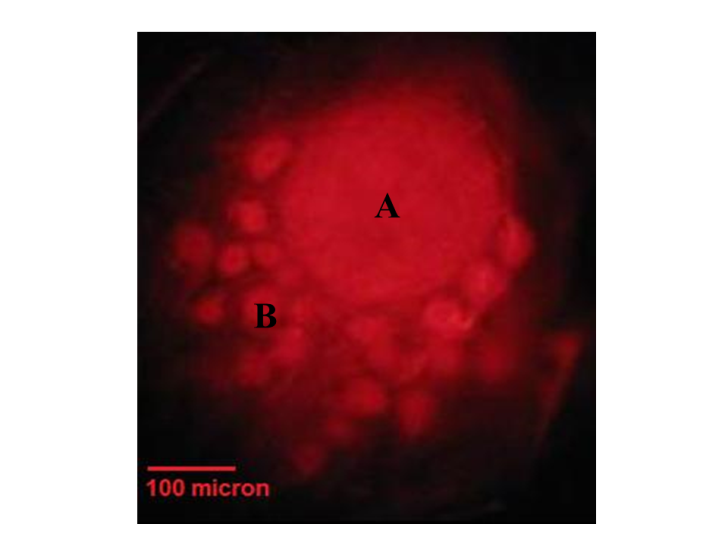
\includegraphics[width=\columnwidth]{graphics/julbdstain.png}
		\caption[Fluorescence image of the stomatogastric ganglion (STG)]{\textbf{Fluorescence image of the stomatogastric ganglion (STG)} of \species{Cancer pagurus} after bathing with a JULBD saline solution. (A) neuropil, (B) an STG neuron.}
		\label{fig:julbdstain}
	\end{center}
\end{figure}

\subsection{Results}
\footnote{These results were also published in \cite{Bai2014}}The sensitivity of the Bodipy dyes, MULBD and JULBD, were compared with that of di-4-ANEPPS. For the comparison, event-triggered averaging was carried out for recordings made with the Bodipy and di-4-ANEPPS dyes that clearly reflected neural activity . The dynamic range for MJULBD was 9.3\% of the di-4-ANEPPS dynamic range and for JULBD it was 30\%. Results shown in figure \ref{fig:julbdrecording} and figure \ref{fig:mjulbdrecording} show the imaging recordings matching the activity of a neuron that ws recorded using an intracellular electrode.

\begin{figure}[H]
	\begin{center}
		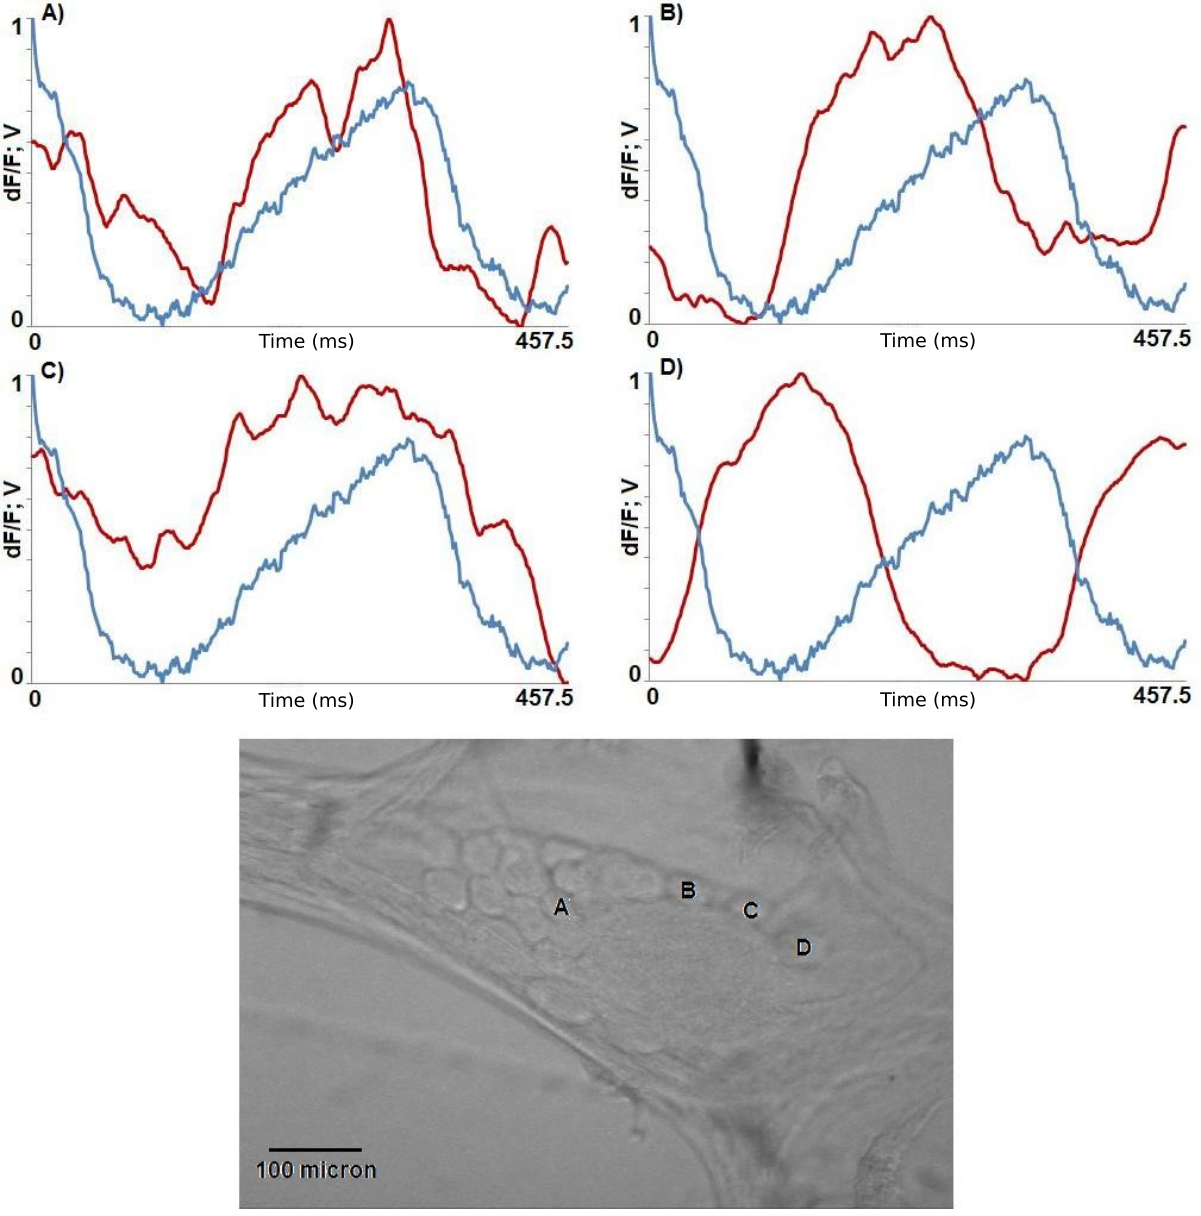
\includegraphics[width=\columnwidth]{graphics/julbdrecording.png}
		\caption[Intracellular and optical \ac{VSD} recording using JULBD of neural activities in the crab STG.]{\textbf{Intracellular and optical \ac{VSD} recording using JULBD of neural activities in the crab STG.} (A) \ac{PY} neuron recorded simultaneously by intracellular and optical \ac{VSD} recording; (B–D) other \ac{STG} neurons recorded only by \ac{VSD} imaging and considered against the reference provided by the intracellular recording of the \ac{PY} neuron shown in (A). The blue traces in all panels show the intracellular electrical recording of the \ac{PY} neuron. The red traces in all panels show the \ac{VSD} fluorescence imaging recording of the corresponding neurons marked in the bottom panel. All shown recording data were calculated using event-triggered averaging as described in the paper. The units on the vertical axes are arbitrary scaled units.}
		\label{fig:julbdrecording}
	\end{center}
\end{figure}
\begin{figure}[H]
	\begin{center}
		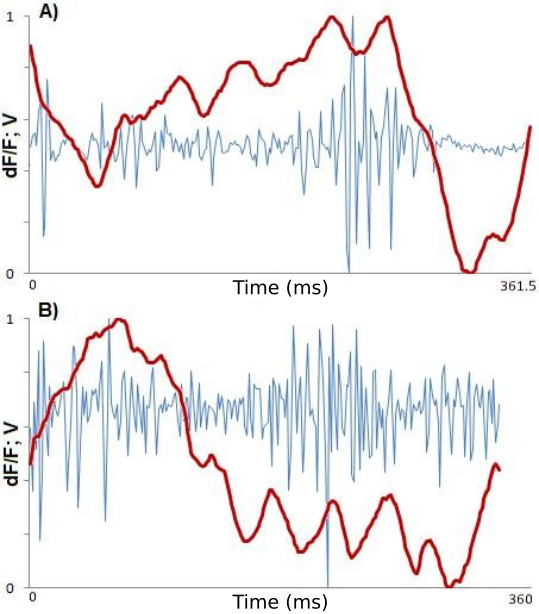
\includegraphics[width=12cm]{graphics/mjulbdrecording.png}
		\caption[Extracellular and optical \ac{VSD} recording using MJULBD of neural activities in the crab \ac{STG}]{\textbf{Extracellular and optical \ac{VSD} recording using MJULBD of neural activities in the crab \ac{STG}}. The blue traces in the panel shows the extracellular recording of full pyloric cycle from the \ac{lvn}. The red traces in the panel shows the \ac{VSD} imaging recording of an \ac{STG} neuron. All shown data were calculated using event-triggered averaging as described in section \ref{sec:detrend}. The units on the vertical axes are arbitrary scaled units}
		\label{fig:mjulbdrecording}
	\end{center}
\end{figure}

Also of interest when developing \acp{VSD} is toxicity. The toxic effect of \acp{VSD}, typically speeds up the pyloric rhythm. The toxic effects of the Bodipy dyes were compared to that of di-4-ANEPPS by measuring the impact of the dye on the pyloric rhythm cycle while the the \ac{STG} preparation was exposed to exciting illumination.

For the analysis recordings made with dye solutions of $10^{-5}$M dye concentration were used. It was found that there was a reduction of cycle length from one cycle to the next of 2.4\% for JULBD. Using a t-test at 5\% significance, this reduction proved to be significantly positive. di-4-ANEPPS and MJULBD however, showed no significant shortening of cycle length.

Over a long period, i.e. several minutes, all dyes prove to have some toxic effect which is reflected by the shortening rhythm cycle length.

\subsection{Discussion}
Zwitterionic dyes such as di-4-ANEPPS and di-8-ANEPPS are the dominating technology for \ac{VSD} imaging. There is, however, still room for improvement  with regards to toxicity, responsivity and signal to noise ratio.

As an alternative to zwitterionic voltage sensitive dyes we investigated the use of dyes based on the Bodipy framework for \ac{VSD} imaging. Our results are the first to demonstrate that Bodipy dyes can be used for neural imaging.

The MJULBD dye gives a much narrower dynamic range for the signal, but it has similar low toxicity as di-4-ANEPPS. Although the fluorescence voltage response of JULBD proved not to be any better than that of 4-ANEPPS, it appears that the BF$_{2}$ group reduces the toxicity of Bipody dyes to neurons \cite{Bai2014}.

\subsection{Conclusion}
The search for methods that would provide a better signal to noise ratio when recording neural activity is ongoing. It is also of vital importance to find methods that would allow the recording of whole networks as recordings from individual or a few neurons do not give sufficient information to understand complete networks. \Acp{VSD} offer a solution but there is still a great deal of research and development to be done to increase the signal to noise ratio and reduce the toxicity of such dyes.

The positive results from the pilot study has resulted in further funding being obtained from the Leverhulme Trust in the amount of ca. \pounds 170K. This study into the development of Bodipy dyes will be a partnership between the laboratories of Prof. Peter Andras from Keele University and Prof. Andrew Benniston from Newcastle University.

\section{Multi-electrode Arrays}
\subsection{Methods}
\label{subsec:MEA}

The possibility exists that \acp{MEA} can be used in conjunction with \acp{VSD}. Potentially simultaneously recording of neural activity with 
both  the \ac{MEA} and \ac{VSD} can be done. \acp{MEA} can also be used to stimulate neurons. Such stimulation would allow us to study the effect of stimulating specific neurons on the known rhythms produced by the central pattern generators found in the \ac{STG}. The main reason for considering the use of the \ac{MEA} and \ac{VSD} would be to overcome the restrictions of traditional electrophysiological methods to record activity of all the neurons of the \ac{STG} simultaneously. 

In collaboration with the laboratory of Prof. George Kemenes, from Sussex University, we investigated the use of a \ac{MEA} on the \ac{STG} of \species{Cancer pagurus}. The deafferented and desheathed \ac{STG} was placed on a \ac{MEA} with 252 electrodes which were 30 $\mu m$ in diameter and spaced 100 $mu$m apart. The nervous system was held in place by a combination of plastic strips, Blu Tack and a glass cover slip.

Neural activity was recorded using MC Rack software produced by MultiChannel Systems. Spike sorting was accomplished using a \matlab script which implements a a centre-of-mass calculation which is described in a paper by Novak and Wheeler \cite{Novak1986}. A 20 $\mu V$ threshold was used to detect spikes in 100Hz high-pass filtered data.

\subsection{Results}
Of six experiments done, the experiment which recorded the most active neural activity was chosen.  Using the  \matlab scripts mentioned in section \ref{subsec:MEA}, 33293 spikes were triangulated in the first 10 minutes of recording. A spike could be triangulated if it was detected on at least three electrodes at an amplitude of 20$\mu V$ or more. A typical recording over one electrode is shown in figure \ref{fig:MEA_recording}.

Figure \ref{fig:MEA_recording} shows a typical recording of the neural activity that was recorded over one electrode. A 5Hz rhythmic pattern can be observed in the recording. At least 23 spatially distinct spike sources were detected. These sources are shown in figure \ref{fig:MEA_analysis1a} and \ref{fig:MEA_analysis2}.

\begin{figure}[H]
	\begin{center}
		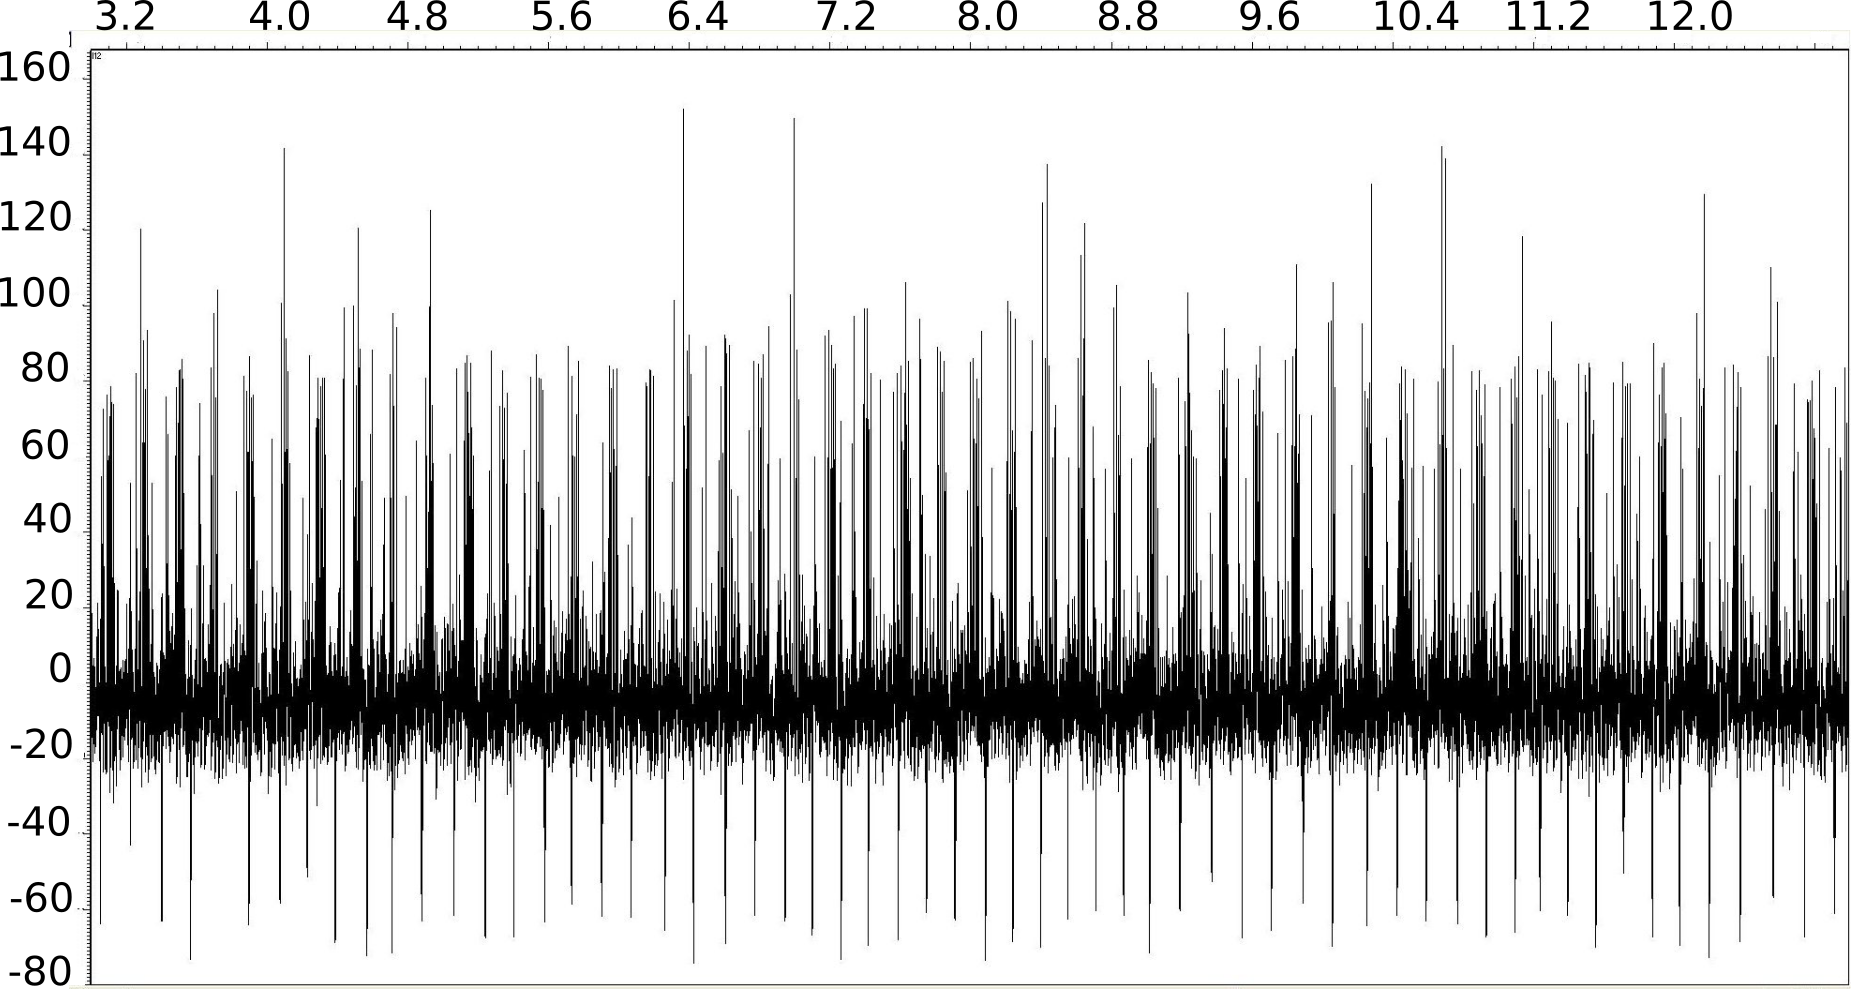
\includegraphics[width=13cm]{graphics/MEA_recording.png}
		\caption[\ac{MEA} Recording]{\textbf{MEA recording. }A typical recording of neural activity over one electrode as recorded with a multi-electrode array. A 5Hz rhythmic pattern could be observed.}
		\label{fig:MEA_recording}
	\end{center}
\end{figure}
\begin{figure}[H]
	\begin{center}
		\includegraphics[width=13cm]{graphics/MEA_analysis1a.png}
		\caption[\ac{MEA} Spike sources detected with a \matlab script.]{\textbf{\ac{MEA} Spike sources detected with a \matlab script.} Each detected spike is shown as circle. The detected spikes are overlaid on the image of the \ac{STG}, showing where on the \ac{STG} the spikes originated. The \acp{aln} and \ac{dvn} are labelled on the image. Figure \ref{fig:MEA_analysis2}, is an enlarged view of the activity.}
		\label{fig:MEA_analysis1a}
	\end{center}
\end{figure}
\begin{figure}[H]
	\begin{center}
		\includegraphics[width=\columnwidth]{graphics/MEA_analysis2a.png}
		\caption[Spike sources detected on \ac{MEA} recording. ]{\textbf{Spike sources detected on \ac{MEA} recording. }At least 23 spatially distinct spike sources were detected. The small red crosses on the image shows the position of the electrodes. Each circle is a spike that was detected in the first 10 minutes of the recording. The colour of the circle reflects a normalised amplitude of the spike.}
		\label{fig:MEA_analysis2}
	\end{center}
\end{figure}

\subsection{Discussion}
To provide insight into neural activity over the whole \ac{STG} we investigated the use of \acp{MEA} as a method of recording. It was found that most spikes and distinct areas of activity were identified over the neuropil which raised the question whether some areas might be neurite segments of the same neuron rather than neurons. To determine whether this is indeed the case further analysis will be required. It has been found that signals recorded over the neuropil are predominantly from the \acp{PD} but it is not possible to confirm whether this was the case with the recordings made for this initial investigation into the use of \acp{MEA}. The equipment used during the investigation, lacked the facility for making an extra-cellular recording which is usually used to identify the timing, and thus the identification of the spiking neuron.

The 5Hz rhythmic activity observed in figure \ref{fig:MEA_recording} was not evident in the spike sorted data. Re-sorting the data at a higher voltage threshold should resolve this discrepancy.

We have shown, however, that it is possible to successfully record from the \ac{STG} using an \ac{MEA}. In terms of hardware, software and protocols, areas were identified that will need refining to successfully use the \ac{MEA}, either independently or in conjunction with \ac{VSD}.

\note{pilot work in vsd design (mention more about our paper), mea and optogenetics.}

\note{How to design rationally the vsd. Basic boron module good for rational molecular design.}

\subsection{Conclusion}
With its added functionality of stimulation, \acp{MEA} could prove of significant value in research on the \ac{STG} as an alternative to \acp{VSD} or even for use in combination with \acp{VSD}. Both these methods allow recording from the whole \ac{STG}. Being able to study the effect of stimulation of one or more neurons or the effect of a modulation on all the neurons at the same time could give us invaluable insight into the workings of \acp{CPG}.

We have shown that we can successfully record from the \ac{STG} using an \ac{MEA}. We have identified areas, in terms of hardware, software and protocols, that will need refining to successfully use the \ac{MEA} in conjunction with \acp{VSD}. 

The equipment that were used for the proof of concept experiments, were from a \species{Lymnea stagnalis} lab, which were not adequately set up for \ac{STG} experiments. Perfusion of the preparation is required to keep the temperature of the saline between 10 and 15 degrees Celsius and can be implemented in the same manner as is used for \ac{VSD} and electrophysiological experiments.

Extra-cellular recordings are of vital importance to be able to identify spiking neurons that are being recorded. In the case of \ac{MEA} setup, a suction electrode has to be used rather than wire electrodes.


\section{Injection of dyes using compressed air}
\subsection{Methods}
\label{subsec:picospritzer}
Yet another method that was investigated is the use of compressed air to inject \ac{VSD} into cells. To our knowledge, this method has not been attempted before for the injection of \ac{VSD} into neurons. The Picospritzer III is a rack mountable system which can supply controlled and repeatable pressure pulses. Rather than using current to drive the dye into the cell, compressed air is pushed into a dye filled glass microelectrode. Glass microelectrodes are pulled as for intracellular recordings and dye fillings but the point of the microelectrode is broken off and polished, using an open flame, to obtain a slightly larger diameter. The electrode is then placed tightly against the cell, but not so that it penetrates the membrane. When the compressed air is pushed into the glass electrode, the dye is injected into the cell.

The glass microelectrodes were pulled using a P-97 Flaming/Brown Micropipette Puller from Sutter Instruments. The following settings on the puller were found to produce microelectrodes with the most appropriate shape with regards to taper and tip size for injection:

\begin{table}[H]
	\centering
	\label{tab:puller}
	\caption{Pipette Puller settings for microelectrodes used for injection with the Picospritzer.}
	\begin{tabular}{c c c c c}
		Ramp & Head & Pull & Velocity & Time/Del \\ \hline
		511 & 511 & 30 & 80 & 250
	\end{tabular}
\end{table}

The duration and pressure of the air injection of the dye is also important. After some experimentation we found the settings as shown in table \ref{tab:injection} to be ideal in that the dye was injected into the cell without damaging the neuron. The viability of the preparation during injection could be confirmed by make sure that the pyloric rhythm which is recorded during injection remains unaltered.

\begin{table}[H]
	\centering
	\caption{Picospritzer settings used for injection of \ac{VSD} into pyloric neurons.}
	\label{tab:injection}
	\begin{tabular}{c c}
		Duration (msec) & Pressure (PSI) \\ \hline
		500 & 30 
	\end{tabular}
\end{table}

\subsection{Results}
Because injection of \ac{VSD} with electrical pulses is so time consuming the neurons are usually identified first in order to fill only neurons specific to the requirements of the experiment. The preparation is not likely to survive the amount of time that would be required to inject all neurons with the electrical pulse method and then to be identified later with imaging data. Injection of \ac{VSD} using the Picospritzer III is an exciting prospect as it allows for instantaneous injection of dye which would otherwise take at least thirty minutes per neuron when using conventional intracellular injection with electrical pulses. It also allows for all visible neurons to be injected without having to identify neurons first as identification can be done afterwards from the imaging data.

Dye was successfully injected into several cells of the \ac{STG} with the cells surviving the injection and the pyloric rhythm maintained. The process of injecting the dye into several cells took less than an hour. It was thus shown that it is also possible to inject many cells in a short period. As many cells as can be seen can be filled to allow recording from as many cells as possible. Avoiding the penetration of cells multiple times (first for identification and then for filling) also reduces the risk of damaging the preparation. 

\subsection{Discussion}
Time did not allow for the refinement of the process for injecting \ac{VSD} using compressed air. However, it was shown in principle that the method should work and possibly provide a much better alternative for filling cells with intracellular \ac{VSD}. Intracellular \ac{VSD} has the advantage of giving a much better signal to noise ratio for better recording of neural activity but the skill required and the amount of time it takes to first identify and then fill a neuron using electrical pulses makes it a very difficult method to use. Injection using compressed air could potentially provide a much easier and quicker method with better results.

\subsection{Conclusion}
The fact that injection with compressed air can be successfully used as a delivery mechanism on neurons of the \ac{STG}, opens up other possibilities such as optogenetics. Optogenetics is already used successfully in model organisms such as \textit{Caenorhabditis elegans} \cite{Husson2013} and \textit{Danio rerio} \cite{DelBene2012}. In these two species genetically altered strains of the organisms are bread for experimentation. In crustacean however, this would not necessarily be an option because these animals take about four years to reach the required size. On the other hand it is possible to keep the deafferented \ac{STNS} alive for at least a week with the use of antibiotics. It has been shown that plasmids can be injected into in tact brains of \species{Xenopus} tadpoles \cite{Hewapathirane2008, Haas2001}. The delivery of appropriate rhodopsin plasmids would allow optical control of \ac{STG} neurons and the analysis of contribution of individual neurons to the overall functionality of \ac{STG} circuits by selectively switching neurons off and on or by driving multiple neurons with set activity patterns. Potentially what can now be done with current or dynamic clamping on a single neuron can then be done optically with multiple neurons. An optimum solution would be the combination of \ac{VSD} imaging with optical control using different wavelength bands.

If rhodopsin plasmids suitable for expression in crustacean can be developed, injection with compressed air could offer a quick and relatively simple way delivering system offering yet another way of recording neural activity from the complete \ac{STG} network.

\section{Concluding Remarks}
%Could either chop this up a bit and use the content in the intro to the alt. methods section, or make this a summary of the alternative methods section as a whole, but rename it something like 'Alternative methods, concluding remarks' or whatever to wrap the chapter up.
\label{sec:alternative_methods}
Traditionally, neural activity in the \ac{STNS} is recorded with electrophysiological methods. For extracellular recordings, petroleum jelly wells are made over a nerve and one electrode is placed inside the well while a second electrode is placed outside the well. Action potentials can then be observed as spikes. Intra-cellular recordings are made by using micro glass electrodes that can penetrate the cell membrane of soma. Although these methods are very effective they do have limitations. For instance, extracellular recording can only show action potentials. It is not possible to see the depolarising and hyper-polarising of the cell and it is also not possible to measure the potential difference in the soma.

Intra-cellular recordings, on the other hand, accurately records the potential differences in the cell, capturing unique waveforms as well as the action potentials that occur when the required threshold is reached. The main drawback of this method is that the number of electrodes that can be inserted into cells at the same time is limited by the skill of the scientist performing the experiment, but mostly by the physical size of the micro manipulators which have to be arranged around a petri dish to hold the micro glass electrodes. With exceptional skill it might be possible to get as many as five electrodes inserted into five neurons. It is not possible to tell which neuron is which when looking at the \ac{STG} and thus, if recordings from specific neurons are required, the recording process is complicated and slowed down by the fact that neurons have to be penetrated with the glass electrode, one by one, until the required one is found.

Because we know that neurons are modulated differentially we need to be able to record from several neurons at the same time, but we also need to be able to record intra-cellularly to be able to see how and when the neuron gets depolarised or hyperpolarised with respect to other neurons. Using bath-applied \ac{VSD} we were able to record from as many as 19 neurons at the same time. Since we now know that we can successfully record from that many neurons our next goal is to reduce the toxicity of the dyes and to improve the signal to noise of such recordings. Intra-cellular application of \ac{VSD} give a better signal to noise ratio but still has the limitation of the amount of neurons that can be filled due to the time-consuming process of filling the soma with the dye.

For the afore mentioned reasons, the search for better recording methods is ongoing. The new recording techniques, however, also require methods for analysis of the data. Some analysis methods that are used for existing recording techniques are adequate but in some cases new methods are required.



	\chapter{Conclusions and Perspectives}
\label{chap:conclusions_perspectives}
%\section{Verifying the biological accuracy of the model}
%\label{sec:model_conclusions}
%SWALES:
% 1) Why interesting / important?
% 2) What's been done so far?
% 3) What's the hole
% 4) What you did
% 5) What you found
% 6) What it means

Existing models of the \ac{STG} include at most four or five neurons, with neurons of the same type, such as the \acp{PY} and \acp{PD}, modelled as a single neuron. With such a configuration it is not possible to model the differential modulation which occurs when \ac{STG} neurons are exposed to \ac{DA}.

This thesis addresses the need for a computational model to better understand the effect of \ac{DA} on individual neurons as part of a larger network. For this research our interest was focused on the \acp{PY} which comprise the pyloric \ac{CPG} in the \ac{STG} of \species{Cancer pagurus}. We have a certain expectation of the network output which is based on previous research. It has been shown that the \acp{PY} which are synchronised under normal conditions become desynchronised when exposed to \ac{DA} \note{\cite{Johnson1993}}.

This project was started with the gathering of experimental data to inform the computational model. Research into the crustacean \ac{STNS} has mainly been done using traditional electrophysiological methods such as intra-cellular recordings made with glass micro-electrodes that are inserted into the soma of the cell, and extra-cellular recordings that are made using suction or wire electrodes. Previous research at the lab of Prof. Peter Andras has shown that \ac{VSD} can be used successfully on the neurons of the \ac{STG}. The use of \ac{VSD} opens the possibility of recording all the neurons of the \ac{STG} at the same time. Such recordings allow us quantify the contribution of individual neurons to the \ac{CPG} rhythms and, in turn, model the network at neuron level.

To find an improved means of recording from the whole \ac{STG}, a great deal of time and effort was spent making \ac{VSD} recordings and investigating alternative means of recording. Analysis of the pyloric \ac{CPG} activity starts with the identification of the beginning of the pyloric rhythm. The rhythm is usually easily identifiable on extracellular recordings over the \ac{lvn} or \ac{dvn}. Identifying the rhythm was done by finding the first \ac{LP} spike\footnote{Physiologically the start of the pyloric rhythm would be the \ac{PD} activity as it is a pacemaker \cite{Harris-Warrick1992}. However, visually it was easier to use the \ac{LP} activity for this purpose. For the sake of analysis and timing it did not matter which neurons were used to identify the beginning of a phase as long as it is used consistently}. The \ac{LP} spikes are usually easily identifiable as the first long spike after a short pause. \ac{DA}, however, affects the amplitudes of the spikes and it often becomes impossible to identify the rhythm in this way. This significantly complicates identifying the phases of the rhythm. A possible solution to this relies on intracellular recordings, made either by using electrophysiology or \ac{VSD}. If at least one pyloric neuron can be positively identified, the beginning of its depolarisation period can be taken as the beginning of the phase. It has been found in \ac{VSD} imaging that the \ac{PD} signal usually dominates the neuropil. If this signal is found to form a recognisable wave it can be used to identify the beginning of the rhythm.

More detailed analysis of extracellular recordings made simultaneously over the \ac{lvn} and \ac{pyn} can also be useful, at least until other methods for recording and the data analysis for these methods become more mature. Such recordings would allow the identification of the individual \acp{PY} in the rhythm. Dissecting the \acp{pyn} requires some skill as the nerves tend to be very fine and can be difficult to dissect from the surrounding tissue in which it is embedded.

To verify the validity of a model we need to show that the model output is reflective of that of the biological system. We thus need to find means of quantifying the output of the biological system. We have described the detrending and triggered averaging methods used for analysing extracellular recordings and we have also proposed new methods for the analysis of \ac{VSD} recordings. The new method works off-line and involves the identification of salient features which are used to profile a waveform specific to a neuron. The features on  profiled waveforms are then used to quantify the extent of de-synchronisation of the neurons of interest, which in our case are the \acp{PY}.

The new analysis methods were successfully applied to recordings made from both bath-applied neurons and neurons that were individually injected with \ac{VSD}. While the methods have been shown to work well off-line, i.e. applied after the recordings have been made, it would be very useful if the methods can be extended to be used on-line. An on-line application would allow for the immediate identification of neurons that, in turn, would allow for the stimulation of individual neurons if the \ac{VSD} is used in conjunction with \ac{MEA} or traditional electrophysiological techniques.

Using established methodology and newly developed methods for analysis of the data as detailed in chapter \ref{chap:methodsAndMaterials} and \ref{chap:analysis} we were able to construct a detailed computational model of the \acp{PY} in the \ac{STG} that would reflect the expected desynchronisation. Hodkin-Huxley's conductance-based, mathematical model was used as the basis for developing the model for this research. Each neuron is represented with two compartments, the soma and the axon. All axons include three channels, $Na$, $K$ and $L$ while the soma had, depending on the neuron type, up to nine channels. As pacemakers for the circuit, the \ac{AB} and \acp{PD} include $Ca^{2+}$ and $KCa$ channels. 

Several existing models were considered. Very early models from the Hartline laboratory \cite{Hartline1979, Warshaw1976} included up to five neurons, however the decision was made to not consider such very old models but to rather focus on later models that used the Hodgkin-Huxley equations with parameters derived from newer experimental results.

The Golowasch \cite{Golowasch1999a} and Soto-Trevino \cite{Soto-Trevino2005} models, although only modelling two neurons each, proved to be the most comprehensive in terms of available parameters. For instance, by creating a two neuron, two compartment model of the \ac{AB} and \ac{PD} neurons Soto-Trevi$\tilde{n}$o could illustrate how the compartments interact to determine the dynamics of the model neurons \cite{Soto-Trevino2005}.  Both these models use Hodgkin-Huxley equations and were thus relatively easily extendible to incorporate multiple copies of the \acp{PD} and \acp{PY} that would allow modification of gap junction parameter values which is required to model the effect of \ac{DA}. The equations and parameter values from the Golowasch and Soto-Trevi$\tilde{n}$o models were thus used as the starting point for the more complete and biologically accurate pyloric \ac{CPG} model presented. 

As is, the model created for this research incorporates two \acp{PD} neurons which means that it is already possible to use the model for research into the effects of various conditions, such as neuromodulation, of the \acp{PD}. The model is also suitable for investigating the impact of different ranges, differences and ratios of conductance parameters with the intentions of determining the impact of these on the pyloric rhythm. For example such investigations may give a better insight into the mechanisms
 charaterising the \ac{STG} behaviour following decentralisation and during the spontaneous re-establishment of the pyloric rhythm.

The effect of \ac{DA} was modelled by adjusting the values of the $K^{+}$ channel parameters and the gap junction strength between the \acp{PY}. Using t-tests which compared the \ac{ISI} of the five \acp{PY} for gap junction strengths of zero to 90 percent (at 10 percent intervals) against the 100 percent strength value of the gap junctions we were able to confirm that model did indeed succeed in showing the expected de-synchronisation of the \acp{PY} under neuromodulatory conditions.

The model produced can easily be extended to include more neurons, junctions and channels with the main challenge being the finding of appropriate parameters. Such parameters depend on the biological measurements which in turn rely on the methods of recording that are available.

As part of this research we also investigated the use of alternative methods to record the  activity of individual neurons, but in a complete neural circuit. Existing methods are extremely limited in this respect. Methods that can simultaneously record from large number of neurons in such a way that the contribution of individual neurons can be isolated has the advantage of showing the contributions that individual neurons make to the whole. Data recorded in such a way would be invaluable to the development of models as we would be able to parametrise neurons  more accurately and thus reflect biologically true activity.

We investigated three alternative methods. These methods were the use of alternative \acp{VSD} in an attempt to improve responsivity, signal to noise ratio and toxicity, which are the main drawbacks of of current \acp{VSD}. We also looked at the use of \acp{MEA} which could potentially allow not only recording of the complete \ac{STG} but also stimulation of neurons. Lastly we investigated the use of the Picospritzer III for injection of substances such as \ac{VSD} and plasmids into neurons of the \ac{STG} using compressed air. Such injection would have the advantage of offering a much faster and safer delivering method, to improve the longevity of \ac{STNS} preparations. In principle, we were able to show that the three methods could be used successfully with further development.

In conclusion this work presents an improvement on current models of the \ac{STG} with implications for medical science. We still lack conclusive evidence of \acp{CPG} in humans. However, Banaie et. al \cite{Banaie2009} was able to use a model to offer a possible explanation for the gait disorder in \ac{HD}. Unfortunately direct research on vertebrate \acp{CPG} has severe limitations due to ethical and practical constraints. Thus work on invertebrate \acp{CPG} can contribute critically to better understanding of vertebrate movement generation. Our work contributes towards better modelling and understanding of neuromodulatory impact on \ac{CPG} functionality with potential implications to the understanding of neurmodulator-related movement disorders (eg. Parkinsons' Disease). 

Neurons of the same type do not necessarily respond exactly in the same way to neuromodulators such as \ac{DA} and each neuron could affect the network differently. Using the \ac{STG} with the pyloric \ac{CPG} as a model system we have been able to show the need for such differentiation to be considered in computational models. Improved quality data is required to build finer and more detailed models. Here we also reported new methods for improved data analysis and proof of concept for alternative methods for more detailed recording of neurons within networks.

\section{Further work}

The research discussed in this thesis leads to new questions that could be investigated with further research in the future:

\begin{itemize}
	\item We showed that we can model the de-synchronisation of the \acp{PY} caused by \ac{DA}. The question that remains is why is such de-synchronisation required. It is known that the pyloric \ac{CPG} produces alternative rhythms \textit{in vivo}. Hypothetically this de-synchronisation is required to switch to an alternative rhythm.
	\item It is known that there are "early" and "late" \acp{PY}, ie. some \acp{PY} fire before the others. The questions is whether the early and late firing of these neurons is a reflection of the parameters. If that is the case we can hypothesize that the early and late \acp{PY} have different effects on the rhythm and this can potentially be tested with the presented model.
	\item It is known that the pyloric rhythm will stop after de-centralisation, i.e. being disconnected from higher higher ganglia. Recovery of the rhythm has been modelled using Hodgkin-Huxley models by altering the Calcium ion current mechanism. However, it is possible that modification of the maximal conductance values of certain ionic currents might also restore  the rhythmic activity of the pyloric network. It should be possible to test this hypothesis by using the presented model with minor alterations.
\end{itemize}

	
	% Appendix
	%\renewcommand{\thechapter} {\Alph{appendix}}
	\appendix
	
	\label{Appendices}
	\begin{appendices}
		
		\chapter{Simple MATLAB Implementation of the Hodgkin Huxley Equations}
\label{app:HH}

\lstset{ %
	backgroundcolor=\color{white},   % choose the background color; you must add \usepackage{color} or \usepackage{xcolor}
	breakatwhitespace=false,         % sets if automatic breaks should only happen at whitespace
	breaklines=true,                 % sets automatic line breaking
	commentstyle=\color{mygreen},    % comment style
	deletekeywords={...},            % if you want to delete keywords from the given language
	escapeinside={\%*}{*)},          % if you want to add LaTeX within your code
	extendedchars=true,              % lets you use non-ASCII characters; for 8-bits encodings only, does not work with UTF-8
	keepspaces=true,                 % keeps spaces in text, useful for keeping indentation of code (possibly needs columns=flexible)
	keywordstyle=\color{blue},       % keyword style
	language=Matlab,                 % the language of the code
	otherkeywords={*,...},            % if you want to add more keywords to the set
	rulecolor=\color{black},         % if not set, the frame-color may be changed on line-breaks within not-black text (e.g. comments (green here))
	showspaces=false,                % show spaces everywhere adding particular underscores; it overrides 'showstringspaces'
	showstringspaces=false,          % underline spaces within strings only
	showtabs=false,                  % show tabs within strings adding particular underscores
	stringstyle=\color{mymauve},     % string literal style
	tabsize=2,                       % sets default tabsize to 2 spaces
}
\begin{lstlisting}

% Parameters in:
%   v0 		initial value of the potential
%   I_ext 	A 1xT vector. It represent the external 
%			current.
% Constants:
%   DT      ms time steps for ode solver
%   C       Membrane capacitance
%   E_L     mV Leakage reversal potential
%   E_Na    mV Na reversal potential
%   E_K     mV K reversal potentsial
%   G_L     mS/cm^2 Leakage conducatance
%   G_Na    mS/cm^2 Na conductance
%   G_L     mS/cm^2 Leakage conductance
function [v h m n]=HHModel(v0,I_ext)
	T=length(I_ext);
	v=zeros(1,T);
	%Constant values
	DT=0.01; 
	C=0.01; 
	E_L=-49.42; 
	E_Na=55.17; 
	E_K=72.14; 
	G_L=0.003; 
	G_Na=1.20; 
	G_K=0.36; 
	g_L=G_L;
	g_Na=zeros(1,T);
	g_K=zeros(1,T);
	m=zeros(1,T);
	n=zeros(1,T);
	h=zeros(1,T);
	m(1)=0.05;
	h(1)=0.54;
	n(1)=0.34;
	v(1)=v0;
	for t=2:T
		v(t)= v(t-1) + (DT/C)*(I_ext(t-1)-g_L*(v(t-1)-E_L)-g_Na(t-1)* ...
		(v(t-1) -E_Na)-g_K(t-1)*(v(t-1)+E_K));
		m(t)=m_fun(m(t-1),v(t-1),DT);
		n(t)=n_fun(n(t-1),v(t-1),DT);
		h(t)=h_fun(h(t-1),v(t-1),DT);
		g_Na(t)=G_Na*(m(t)^3)*h(t);
		g_K(t)=G_K*(n(t)^4);
	end

function y=alpha_n(V)
	y=(0.1 -0.01*(V+65)) ./(exp(1-0.1*(V+65))-1);

function y=alpha_m(V)
	x=2.5 -0.1*(V+65);
	y=x ./(exp(x)-1);

function y=alpha_h(V)
	y=0.07*exp(-(V+65)/20);

function y=beta_n(V)
	y=0.125 * exp(-(V+65)/80);

function y=beta_m(V)
	y=4 * exp(-(V+65)/18);

function y=beta_h(V)
	y=1 ./(exp(3-0.1*(V+65))+1);

function n=n_fun(n0,v,t)
% n0 is the initial value of n
% v is the constant value of the potential
% t is the time.
	n_0=1 ./(1 + beta_n(v) ./ alpha_n(v));
	tau_n=1 ./(alpha_n(v) +beta_n(v));
	n=n_0 -(n_0 -n0)*exp(-t/tau_n);

function m=m_fun(m0,v,t)
% m0 is the initial value of m
% v is the constant value of the potential
% t is the time.
	m_0=1 ./(1 + beta_m(v) ./ alpha_m(v));
	tau_m=1 ./(alpha_m(v) +beta_m(v));
	m=m_0 -(m_0 -m0)*exp(-t/tau_m);

function h=h_fun(h0,v,t)
% h0 is the initial value of h
% v is the constant value of the potential
% t is the time.
	h_0=1 ./(1 + beta_h(v) ./ alpha_h(v));
	tau_h=1 ./(alpha_h(v) +beta_h(v));
	h=h_0 -(h_0 -h0)*exp(-t/tau_h);


tic
% initialise pulse vector with zeros
I_ext_Pulse=zeros(1,5000);
% set pulse at 10 for time steps 500 to 700 to initiate action potential
I_ext_Pulse(500:700)=10;
v=HHmodel(-65,I_ext_Pulse);
plot(v)
toc
\end{lstlisting}

		
		\chapter{Dissection}{B}
\label{app:dissection}
Dissection of the crab is done in two parts; first the gross dissection and then the fine dissection. During the gross dissection the entire stomach is removed from the crab, and during the fine dissection the \ac{STNS} is extracted from the stomach and pinned in a Petri dish. During both parts of the dissection the preparation is kept cool by replacing the saline every 10 minutes with fresh saline from the fridge. A basic anatomy of the  whole crab and the stomach is shown in figure \ref{fig:dissectionimage} and \ref{fig:stomach}.

\begin{figure}[H]
	\begin{center}
		\includegraphics[width=8cm]{graphics/dissectionimage.png}
		\caption{The basic anatomy of the crab showing the location of the stomach. (Adapted from \cite{Stein2009})}
		\label{fig:dissectionimage}
	\end{center}
\end{figure}

\begin{figure}[H]
	\begin{center}
		\includegraphics[width=9cm]{graphics/stomach.png}
		\caption{The stomach of the crab with the \ac{STNS}. (Adapted from \cite{Stein2009})}
		\label{fig:stomach}
	\end{center}
\end{figure}



\section{Gross dissection}
The dissection process is started by anaesthetising a crab on ice for about 30 to 45 minutes. A dissection pan is laid out with the tools required, which are; rongeurs, a tapered edge spatula, small scissors, toothed forceps and a black Sylgard-coated dish. Insect pins are used to pin the preparation down. Crab saline (Table \ref{tab:saline}) is also required. Gloves are worn when handling the crabs.

% Table generated by Excel2LaTeX from sheet 'Sheet1'
\begin{table}[H]
	\centering
	\caption{\species{Cancer pagurus} saline}
	\label{tab:saline}
	\begin{tabular}{lrrrrr}
		\hline 
		\textbf{Salt} & \textbf{(mM)} & \textbf{g/Liter} & \textbf{g/2 Liter} & \textbf{g/5 Liter} & \textbf{g/8 Liter} \\ \hline
		KCl   & 11.00    & 0.83  & 1.66  & 4.15  & 6.64 \\
		NaCl  & 440.00   & 25.80  & 51.60  & 129.00   & 206.40 \\
		CaCl2H2O & 13.00    & 1.90   & 3.80   & 9.50   & 15.20 \\
		MgCl26H2O & 26.00    & 5.30   & 10.60  & 26.50  & 42.40 \\
		Trizma base & 11.2  &  1.50  &  3.00  &  7.30  &  12.00 \\
		Maleic Acid &  5.00  &  0.60  &  1.20  &  3.00  &  4.80 \\
		Hepes &  10.00 &  2.38 &  4.76 &  9.52 & 19.04 \\
		\multicolumn{6}{l}{\textit{(Hepes can be used instead of Tris+Maleate)}} \\
		\hline
	\end{tabular}%
\end{table}%

The first step is to remove the claws and legs using rongeurs or manually (Fig. \ref{fig:dissection_crab2}).

\begin{figure}[H]
	\begin{center}
		\includegraphics[width=9cm]{graphics/dissection_crab2.png}
		\caption{First step of dissections is to remove the claws and legs using rongeurs or manually.}
		\label{fig:dissection_crab2}
	\end{center}
\end{figure}

The external mouth parts are removed next. Using the rongeurs the large external mandibles are removed first and then the smaller 1st and 2nd maxillipeds, exposing the 2nd maxillae which covers the opening to the oesophagus. The 2nd maxillae are attached to thin long ossicles with a muscle attached to the end. These are removed, using the rongeurs, with a twist and pull motion.

The rongeurs are then used to break off the carapace edges on both sides by starting at the lateral posterior end and working towards, and up to the eyes. A gap is created between the dorsal and ventral carapace, exposing the hypodermis (Fig. \ref{fig:dissection_crab3}).

\begin{figure}[H]
	\begin{center}
		\includegraphics[width=9cm]{graphics/dissection_crab3.png}
		\caption{Removing the frilled edge on the side of the carapace, exposing the hypodermis underneath.}
		\label{fig:dissection_crab3}
	\end{center}
\end{figure}

Eyes, antennae and rostrum are chipped away leaving a thin layer of carapace intact that can later be easily broken by hand. 

The hypodermis is then separated from the carapace, holding the spatula against carapace so as to not put pressure on the tissue below in which the \ac{STNS} is embedded (Fig. \ref{fig:dissection_crab4}).

\begin{figure}[H]
	\begin{center}
		\includegraphics[width=9cm]{graphics/dissection_crab4.png}
		\caption{The hypodermis is separated from the carapace taking care not to damage the tissue below the carapace where the nervous system is located.}
		\label{fig:dissection_crab4}
	\end{center}
\end{figure}

The carapace is removed in three sections (Fig. \ref{fig:dissection_crab_sections}). The triangular shapes on the sides are removed first (Fig. \ref{fig:dissection_crab5}). The tapered edge of the spatula is then used again to separate the hypodermis from the centre part that is left over when side sections have been removed. %(Fig \ref{fig:dissection_crab6}). 
The hypodermis is separated from the carapace as far forward (anteriorly) as possible and as far back (posteriorly) as the two ossicles that protrude from the carapace. The centre part of the carapace is then be removed by breaking the connecting strip  of carapace parallel to the posterior and between the two  corners of the triangular shaped sections. This section is then removed manually by bending it upwards towards the anterior, exposing almost all of the hypodermis on the dorsal side of the crab (Fig. \ref{fig:dissection_crab7}).

\begin{figure}[H]
	\begin{center}
		\includegraphics[width=9cm]{graphics/dissection_crab_sections.png}
		\caption{The carapace is removed in three sections.}
		\label{fig:dissection_crab_sections}
	\end{center}
\end{figure}
\begin{figure}[H]
	\begin{center}
		\includegraphics[width=9cm]{graphics/dissection_crab5.png}
		\caption{Firstly the triangular shaped section to the sides are removed.}
		\label{fig:dissection_crab5}
	\end{center}
\end{figure}

\begin{figure}[H]
	\begin{center}
		\includegraphics[width=9cm]{graphics/dissection_crab6.png}
		\caption{The centre part of the carapace should be separated from the hypodermis until one can see through the opening.}
		\label{fig:dissection_crab6}
	\end{center}
\end{figure}
\begin{figure}[H]
	\begin{center}
		\includegraphics[width=9cm]{graphics/dissection_crab7.png}
		\caption{The last section of carapace to be removed is the centre part.}
		\label{fig:dissection_crab7}
	\end{center}
\end{figure}

The tapered edge of the spatula is then used to separate ventral tissue from the carapace. Tissue at the cephalon is drawn back exposing the connecting tissue (Fig. \ref{fig:dissection_crab8}). The connecting tissue is then cut with the scissors allowing the tissue to be drawn back even further - up to the point where the oesophagus is attached to the ventral side of the carapace is exposed (Fig. \ref{fig:dissection_crab9}).

\begin{figure}[H]
	\begin{center}
		\includegraphics[width=9cm]{graphics/dissection_crab8.png}
		\caption{Separate the ventral tissue from the carapace and push the tissue below the eyes as far back as the connecting tissue.}
		\label{fig:dissection_crab8}
	\end{center}
\end{figure}
\begin{figure}[H]
	\begin{center}
		\includegraphics[width=9cm]{graphics/dissection_crab9.png}
		\caption{The connecting tissue is cut using the scissors and push the tissue back up to where the top oesophagus is exposed.}
		\label{fig:dissection_crab9}
	\end{center}
\end{figure}

The labrum is detached from the epistome using small scissors. The cephalum is then removed making diagonal breaks from next to the eyes down to the oesophagus (Fig. \ref{fig:dissection_crab10})

\begin{figure}[H]
	\begin{center}
		\includegraphics[width=9cm]{graphics/dissection_crab10.png}
		\caption{The cephalum is removed after the oesophagus is loosened from the carapace and then diagonal breaks are made from the eyes to the oesophagus.}
		\label{fig:dissection_crab10}
	\end{center}
\end{figure}

The crab is then propped up on the side of the dissection pan using the claws. While the labrum is held in place with the forceps the stomach is extracted by cutting it away from the ventral carapace (Fig. \ref{fig:dissection_crab11}).

\begin{figure}[H]
	\begin{center}
		\includegraphics[width=9cm]{graphics/dissection_crab11.png}
		\caption{The crab is propped up on the side of the dissection pan using the claws. While the labrum is held in place with the forceps the stomach is extracted by cutting it away from the ventral carapace.}
		\label{fig:dissection_crab11}
	\end{center}
\end{figure}

The stomach is then removed from the body and laid down the back of the hand with the hypodermis facing down (Fig. \ref{fig:dissection_crab12}). 
\begin{figure}[H]
	\begin{center}
		\includegraphics[width=9cm]{graphics/dissection_crab12.png}
		\caption{The stomach is removed from the body and laid down the back of the hand with the hypodermis facing down.}
		\label{fig:dissection_crab12}
	\end{center}
\end{figure}
Excess tissue is scraped off and then the stomach is filled with saline to inflate it. Inflating the stomach with saline makes it easier to enter the scissors into the oesophagus to cut through the top layer of the stomach from the oesophagus to the pylorus and through the ossicle between the ampullae (Fig. \ref{fig:dissection_crab13}). 
\begin{figure}[H]
	\begin{center}
		\includegraphics[width=9cm]{graphics/dissection_crab13.png}
		\caption{A cut is made from the oesophagus to the pylorus.}
		\label{fig:dissection_crab13}
	\end{center}
\end{figure}
Two diagonal cuts are made through the cardial branches, which allows the stomach to open up and expose the three teeth inside. The tips of three teeth are cut off (Fig. \ref{fig:dissection_crab14}) which allows the stomach to lie flat when placed in a dish with black Sylgard and the inside of the stomach facing down. The dish is filled with cold crab saline before the stomach is placed in it. The stomach lining is pinned down tightly using dissection pins (Fig. \ref{fig:dissection_crab15}).
\begin{figure}[H]
	\begin{center}
		\includegraphics[width=9cm]{graphics/dissection_crab14.png}
		\caption{The tips of the three teeth are cut off.}
		\label{fig:dissection_crab14}
	\end{center}
\end{figure}
\begin{figure}[H]
	\begin{center}
		\includegraphics[width=9cm]{graphics/dissection_crab15.png}
		\caption[Pinned-down stomach. ]{\textbf{Pinned-down stomach. }The opened stomach is pinned down flat in a dish with black Sylgard. The inside of the stomach faces down. Before the stomach is placed in the dish the dish is filled with crab saline. }
		\label{fig:dissection_crab15}
	\end{center}
\end{figure}

\section{Fine dissection}

For the fine dissection the following additional equipment is needed, a stereoscopic microscope with zoom capability, a 3.5 inch clear Sylgard coated petri dish, two size 5 forceps, dissecting scissors, small dissection pins, fine dissection pins and saline.

When viewed from above the dissected stomach is covered with hypodermis. More or less in the middle of the preparation there are two small dots. All of the hypodermis is cut away leaving only a small circle of tissue around the two dots.

% (Fig. \ref{fig:finedissection_crab01})
%\begin{figure}[H]
%	\begin{center}
%		\includegraphics[width=9cm]{graphics/figure_x.png}
%		\caption{Cut all of the hypodermis away leaving only a small circle around the two dots in the middle of the prep.}
%		\label{fig:finedissection_crab01}
%	\end{center}
%\end{figure}
To the anterior of the small piece of hypodermic tissue left behind, is the brain. From the brain there are two thick nerves, the \ac{coc} nerves. Covering these nerves is a layer of light yellow tissue, which when cut away, makes it possible to see the \ac{coc} well enough through the. Starting at the brain the \acp{coc} are exposed by following them and cutting the tissue above to expose the nerve. The nerve is followed to expose the \acp{CoG} and the rest of the nerve to the anterior of the preparation where the nerve ends. All tissue to the posterior of the \acp{coc} is cleared away. The brain is then lifted and the tissue below the brain and above the opthalmic artery is cut away. The \acp{coc} are then cut against the brain and the brain is removed. Once the brain is removed it is possible to see the opthalmic artery clearly. The opthalmic artery splits to form a 'Y'. By grasping the artery with the forceps to the posterior of the split it is possible to lift the artery and see where the \ac{stn} leaves the artery and bends downward. The artery is cut as close to the \ac{stn} as possible and is then removed by cutting it away from the tissue below and cutting it loose from the ossicles to the the anterior. With the artery removed it is possible to the see the \ac{OG} and the \acp{ion}. To clear the \acp{ion} they are followed from both the \ac{OG} and \acp{CoG}. As one follows the \acp{ion} to be cleared, care has to be taken to notice the where the labral nerve splits off. All tissue between the \acp{ion} is cleared away ass well as the tissue to the anterior of the ions.

At this point in the dissection it is also possible to see the \acp{son} splitting of the \ac{stn}. The \acp{son} can be followed and exposed from the \ac{stn} towards the \acp{CoG}. The tissue between the \acp{son} and \acp{ion} can be clear away leaving only the exposed nerves behind. The \acp{dpon} split off the \ac{son} and care has to be taken to leave at least a short stub of the \ac{dpon} behind for pinning the preparation down in the petri dish later on.

It is now also possible to clear away all orange coloured glandular tissue to the sides of the ac{stn}, posteriorly of the \acp{son}. The are below the \ac{stn} is covered by white tissue that resembles white "wadding" (the material used to stuff padded clothing). The \acp{mvn} run below the orange glandular tissue and on the edge of the white tissue. About two to three centimetres of the \acp{mvn} are cleared. It can sometime be quite difficult to see the white nerves running inside this white tissue but by zooming in on the nerves it is possible to follow the \ac{dvn} (the nerve projecting posteriorly from the \ac{STG}). The \ac{dgn} usually projects out of the \ac{STG} or splits off the \ac{dvn} and then bends downwards towards the dorsal side of the preparation. One to two centimetres of the \ac{dgn} is left in tact and cleared. The \ac{dvn} splits into two ac{lvn}, both which have to be exposed by following them to the posterior and, if possible, to where they split into the \ac{pyn} and \ac{pdn}

Once all these nerves are exposed, care is taken to cut the nervous system away from any tissue that might still be attaching it to the tissue ventrally of the \ac{STNS}. If not already detached, the ends of the \acp{coc}, labral nerves, \acp{dpon}, \acp{mvn}, \ac{dgn} and \ac{lvn},\acp{pyn}, \acp{pdn} are cut loose. The whole \ac{STNS} can now be lifted by grasping it by the ends of the \ac{coc} and the \acp{lvn} and moving it to the side of the dish. The left over stomach lining is unpinned and used to rub it over the Sylgard lined petri dish. Sylgard is hydrophobic and the water will form puddles and not spread evenly over the Sylgard if it is not conditioned in this way with the stomach. Also, without the conditioning the nerves will strongly adhere to the Sylgard and become impossible to handle without damaging. The Petri dish is then rinsed in filled with saline. Grasping the nerves as before, the nervous system is then transferred into the Petri dish. The \ac{STNS} is pinned down onto the Sylgard using minuten pins.

The \ac{STG} can now be exposed by grasping the hypodermis that was left behind with the forceps and lifting it up. This exposes an opening into the ophthalmic artery. The artery is split open by entering the scissors into the artery opening and cutting from the posterior to the anterior between the two dots on the hypodermis. The cut has to be made all the way to the anterior where the artery was cut earlier. Because the artery tissue can be quite tough the artery is sometimes pinned down to the sides to create enough tension for the scissors to cut. The cuts are made while slightly pulling upwards to avoid touching or damaging the STG and the \ac{stn} which runs along the bottom of the artery. Once the \ac{stn} and ac{STG} are exposed the excess artery and hypodermic tissue can be cut away to only leave behind the exposed nerves. Care is taken when the tissue is cut away to leave small stubs of \acp{aln} behind which are required to pin down the \ac{STG}. Without the \acp{aln} it is very difficult to pin the \ac{STG} down sufficiently when desheathing the \ac{STG}.

All excess tissue is cleared away from the \ac{STNS}.




	\end{appendices}
	
	\bibliographystyle{acm}
	\cleardoublepage
	\pdfbookmark{References}{bib}
	\bibliography{research}
	\addcontentsline{toc}{chapter}{References}
	
	
\end{document}
